% This is samplepaper.tex, a sample chapter demonstrating the
% LLNCS macro package for Springer Computer Science proceedings;
% Version 2.20 of 2017/10/04
%
\documentclass[runningheads]{llncs}
%
\usepackage{graphicx}
%% \usepackage[appendix=strip]{apxproof}%default
\usepackage[appendix=append]{apxproof}%default
\graphicspath{
  %% {fig/exp1/}
  {fig/new/}
  {fig/spire2024/}
}%%画像のパス.末尾は'/'で終わること
%% \usepackage[appendix=append]{apxproof}%default
%% \usepackage[appendix=inline]{apxproof}%default

% Used for displaying a sample figure. If possible, figure files should
% be included in EPS format.
%
% If you use the hyperref package, please uncomment the following line
% to display URLs in blue roman font according to Springer's eBook style:
% \renewcommand\UrlFont{\color{blue}\rmfamily}

%%%%%%%%%%%%%%%%%%%%%%%%%%%%%%%%%%%%%%%
%%% macros
%% %%% config.tex

%%======================================
\usepackage{graphicx}
%% \usepackage{amsmath,amssymb}
%% \usepackage{mathtools}
%% \mathtoolsset{showonlyrefs=false} %% 参照している式参照のみ表示
%% \mathtoolsset{showonlyrefs=true} %% 参照している式参照のみ表示
%% \usepackage{cite}
\usepackage{caption}    %%for subfigure
\usepackage[skip=0.5ex]{subcaption} %%for subfigure
\captionsetup{aboveskip=0.0\baselineskip}
\captionsetup{belowskip=0.0\baselineskip}
%%%
%%\usepackage{titlesec}
%% \titlespacing*{\section}{0pt}{5.5ex plus 1ex minus .2ex}{4.3ex plus .2ex}
%% \titlespacing*{\subsection}{0pt}{5.5ex plus 1ex minus .2ex}{4.3ex plus .2ex}

%%% table
%% \usepackage{multirow}
\usepackage{booktabs}
\usepackage{array}

% private macros by others 
\usepackage{url}
\usepackage{bm}
\usepackage{textcomp}%%for cent
%\usepackage[margin=1.75in]{geometry}
%\usepackage[margin=1.0in]{geometry}
%% \usepackage{subfig}
%% \usepackage{natbib}

%%% private %%%%%%%%%%%%%%%%%%%%%%%%%%%%%%%%%%%%%

%% private macros by arim@ist
%%% jsvmac.tex
%%% macros from a subset of jsv1.sty 

%%% from jsv1.sty

% Write multichar identifier names using \id in either mathmode or text;
% For ex, $\id{high}(x)$ is an expression using the \id{high} function.
% Use ``\ '' if a space is desired, as in math mode.
\def\id#1{\ensuremath{\mathit{#1}}}
\let\idit=\id
\def\idbf#1{\ensuremath{\mathbf{#1}}}
\def\idrm#1{\ensuremath{\mathrm{#1}}}
\def\idtt#1{\ensuremath{\mathtt{#1}}}
\def\idsf#1{\ensuremath{\mathsf{#1}}}
\def\idcal#1{\ensuremath{\mathcal{#1}}}  % Use with capital letter args only
\def\idsc#1{\ensuremath{\textsc{#1}}} % added by arim

%%% end jsv1.sty

%%% EOF

%%\input{arimmacro} %%privatemacro


%%%%%%%%%%%%%%%%%%%%%%%%%%%%%%%%%%%%%%%%
%%xsavebox
\usepackage{xsavebox}

%%%%%%%%%%%%%%%%%%%%%%%%%%%%%%%%%%%%%%%%%
%%% above and below float figure table
\setlength\intextsep{0.5\baselineskip}
\setlength\abovecaptionskip{0.0\baselineskip}
\setlength\belowcaptionskip{0.5\baselineskip}
%% \setlength\intextsep{18pt}

%%%%%%%%%%%%%%%%%%
%% latex native savebox and lrbox
\newenvironment{savethm}[1]{\begin{lrbox}{#1}\begin{minipage}[t]{1.0\textwidth}}{\end{minipage}\end{lrbox}}

\newcommand{\putthm}[1]{
%% \smallskip
\noindent 
\usebox{#1}
\medskip}

%%sample
%% \newsavebox{\thmbox}
%% \begin{lrbox}{\thmbox}
%% \begin{minipage}[t]{1.0\textwidth}
%% \begin{theorem}\label{thm:algbwt:main}
%% ....
%% \end{theorem}
%% \end{minipage}
%% \end{lrbox}


%% \putthm{\thmbox}


%%%%%%%%%%%%%%%%%%




%%%%%%%%%%%%%%%%%%%%%%%%%%%%%%%%%%%%%%%%
%%comment out a paragraph
\newsavebox{\cmbox}
\newenvironment{commbox}{
  \begin{lrbox}{\cmbox}
    \begin{minipage}{.9\textwidth}
}{\end{minipage}
  \end{lrbox}
  %\framebox{\usebox{\cmbox}}
}


%%%%%%%%%%%%%%%%%%%%%%%%%%%%%%%%%%%%%%%%
% %%% empty environment 
% \newenvironment{myempty}{\begin{commbox}}{\end{commbox}}
% %%% proof environment 
% \newenvironment{myproof}{\begin{proof}}{\end{proof}} %default
% \newenvironment{myfullproof}{\begin{proof}}{\end{proof}} %default
% \newenvironment{myfullproofempty}{\begin{myempty}}{\end{myempty}} %default

%% replace an enviroment #1 with #2
\newcommand{\myenvironmentreplace}[2]{\renewenvironment{#1}{\begin{#2}}{\end{#2}}}

%% claim %%
\newenvironment{myclaim}[1][]{\bgroup\parskip=0mm\par (\textit{Claim{#1}})}{(\textit{End of Claim})\par\egroup}  
\newenvironment{proofofclaim}{\bgroup\parindent=1em\parskip=0mm\par (\textit{Proof for the claim})}{(\textit{End of the proof for the claim})\par\egroup}  
\newenvironment{proofofclaimempty}{\begin{myempty}}{\end{myempty}}

%% \newenvironment{proofofclaim}{\bgroup\parskip=0mm\par (Proof for the claim)}{(End of the proof for the claim)\par\egroup}  


%%%%%%%%%%%%%%%%%%%%%%%%%%%%%%%%%%%%%%%%

% %% switch catcode of '&' between 4 and 9
% \newenvironment{inalign}{\begin{math}\catcode`&=9}{\catcode`&=4\end{math}}

%%%%%%%%%%%%%%%%%%%%%%%%%%%%%%%%%%%%%%%%

% lipics predefined

%% send a proof to the appendix
\newtheorem{definition}{Definition}
\newtheorem{theorem}{Theorem}
\newtheorem{lemma}[theorem]{Lemma}
\newtheorem{proposition}{Proposition}
\newtheorem{corollary}[theorem]{Corollary}
\newtheorem{remark}{Remark}
\newtheorem{fact}{Fact}
\newtheorem{condition}{Condition}

% \newtheorem{example}[example]{Example}[section]
% \newtheorem{conjecture}{Conjecture}
% %% dammy
%%%%%%%%%%%%%%%%%%%%%%%%%%%%%%%%%%%%%%%%

%%% cleveref
\usepackage{cleveref}
\crefname{section}{Sec.}{Sections}
\crefname{chapter}{Chapter}{Chapters}
%%
\crefname{algorithm}{Algorithm}{Algorithms}
\crefname{table}{Table}{Tables}
\crefname{figure}{Fig.}{Figures}
%% 
\crefname{definition}{Definition}{Definitions}
\crefname{lemma}{Lemma}{Lemmas}
\crefname{proposition}{Prop.}{Propositions}
\crefname{theorem}{Theorem}{Theorems}
\crefname{remark}{Remark}{Remarks}
\crefname{fact}{Fact}{Facts}
\crefname{condition}{Condition}{Conditions}
\crefname{problem}{Problem}{Problems}
\crefname{observation}{Observation}{Observations}
%% \crefname{lemma}{Lemma}{Lemmas}
\crefname{equation}{Eq.}{Equations}
%%% fix of a bug in Algorithm
\newcommand{\aref}[1]{Algorithm\kern0.25em\ref{#1}} 
%%%%%%

% %% send a proof to the appendix
\usepackage{apxproof}
% \newtheoremrep{definition}{Definition}[section]
\newtheoremrep{lemma}[theorem]{Lemma}[section]
\newtheoremrep{proposition}[proposition]{Proposition}[section]
\newtheoremrep{theorem}[theorem]{Theorem}[section]
\newtheoremrep{corollary}[theorem]{Corollary}[section]
% \newtheoremrep{remark}[theorem]{Remark}

%% \newtheoremrep{example}[example]{Example}[section]
%% \newtheoremrep{conjecture}{Conjecture}
%% %% dammy
%% \newcommand{\resetrep}{}
%% rest 
%% \newcommand{\resetreptext}{{\rm\textsf{in draft}}}
%% \newcommand{\getfollow}[1][{}]{{\rm\textsf{(*{#1})}}\ }

%% \newcommand{\resetrep}{%% resetting all rep-style environments
%% %% \renewenvironment{lemmarep}{\begin{lemma}\getfollow}{\end{lemma}}
%% \renewenvironment{lemmarep}{\begin{lemma}\getfollow}{\end{lemma}}
%% \renewenvironment{propositionrep}{\begin{proposition}\getfollow}{\end{proposition}}
%% \renewenvironment{theorem}{\begin{theorem}\getfollow}{\end{theorem}}
%% \renewenvironment{corollaryrep}{\begin{corollary}\getfollow}{\end{corollary}}
%% \renewenvironment{examplerep}{\begin{example}\getfollow}{\end{example}}
%% \renewenvironment{remarkrep}{\begin{remark}\getfollow}{\end{remark}}
%% \renewenvironment{conjecturerep}{\begin{conjecture}\getfollow}{\end{conjecture}}
%% \renewenvironment{toappendix}{}{}
%% }

%%%%% 
\newenvironment{statement}[1]{\begin{trivlist}\item[]$\blacktriangleright\:$\textbf{#1}\ }{\end{trivlist}}
\newenvironment{notoappendix}{}{} %% the empty version of toappendix

%%%%%%%%%%%%%%%%%%%%%%%%%%%%%%%%%%%%%%%%%
%% enumitem: smart enumerate and itemize
%% the vspace above list = \topsep + \parskip + \partopsep
%% the vspace between items = \itemsep + \Parsep 
%% the vspace between paragraphs = \Parsep 
\usepackage[inline,shortlabels]{enumitem} %enumerate
\setlist{noitemsep}
\setlist{%
topsep = 0.25\baselineskip,
parsep = 0.125\baselineskip
}%exp
\setlist[enumerate]{ labelsep=.25pc, leftmargin=1.5pc } 
%% \setlist[enumerate]{ labelsep=.25pc, leftmargin=1.5pc } 
\setlist[enumerate,1]{ label= (\arabic*), ref=\arabic*}
\setlist[enumerate,2]{ label= (\roman*),ref  = \roman*}
\setlist[enumerate,3]{ label= (\alph*), ref  = (\alph*)}
%\setlist[itemize]{ leftmargin=1.5pc }
\setlist[description]{ font=\sffamily\bfseries }
%% end macros
%%% switch
%% \newenvironment{myenumerate}{\begin{enumerate}}{\end{enumerate}}
\newenvironment{myenumerate}{\begin{enumerate*}}{\end{enumerate*}}
%% end macros

%%

%% %% 目次のハイパーリンク: 印刷時は念の為コメントアウト(本来出ない)
%% \usepackage[%
%% %dvipdfmx,%
%% colorlinks=true,%
%% linkcolor=blue,%
%% anchorcolor=black,%
%% citecolor=blue,%
%% urlcolor=blue%
%% ]{hyperref} %注意:パッケージの最後に読み込むこと

%%%%

%% EOF

%%% config.tex

%%======================================
\usepackage{graphicx}
%% \usepackage{amsmath,amssymb}
%% \usepackage{mathtools}
%% \mathtoolsset{showonlyrefs=false} %% 参照している式参照のみ表示
%% \mathtoolsset{showonlyrefs=true} %% 参照している式参照のみ表示
%% \usepackage{cite}
\usepackage{caption}    %%for subfigure
\usepackage[skip=0.5ex]{subcaption} %%for subfigure
\captionsetup{aboveskip=0.0\baselineskip}
\captionsetup{belowskip=0.0\baselineskip}
%%%
%%\usepackage{titlesec}
%% \titlespacing*{\section}{0pt}{5.5ex plus 1ex minus .2ex}{4.3ex plus .2ex}
%% \titlespacing*{\subsection}{0pt}{5.5ex plus 1ex minus .2ex}{4.3ex plus .2ex}

%%% table
%% \usepackage{multirow}
\usepackage{booktabs}
\usepackage{array}

% private macros by others 
\usepackage{url}
\usepackage{bm}
\usepackage{textcomp}%%for cent
%\usepackage[margin=1.75in]{geometry}
%\usepackage[margin=1.0in]{geometry}
%% \usepackage{subfig}
%% \usepackage{natbib}

%%% private %%%%%%%%%%%%%%%%%%%%%%%%%%%%%%%%%%%%%

%% private macros by arim@ist
%%% jsvmac.tex
%%% macros from a subset of jsv1.sty 

%%% from jsv1.sty

% Write multichar identifier names using \id in either mathmode or text;
% For ex, $\id{high}(x)$ is an expression using the \id{high} function.
% Use ``\ '' if a space is desired, as in math mode.
\def\id#1{\ensuremath{\mathit{#1}}}
\let\idit=\id
\def\idbf#1{\ensuremath{\mathbf{#1}}}
\def\idrm#1{\ensuremath{\mathrm{#1}}}
\def\idtt#1{\ensuremath{\mathtt{#1}}}
\def\idsf#1{\ensuremath{\mathsf{#1}}}
\def\idcal#1{\ensuremath{\mathcal{#1}}}  % Use with capital letter args only
\def\idsc#1{\ensuremath{\textsc{#1}}} % added by arim

%%% end jsv1.sty

%%% EOF

%%\input{arimmacro} %%privatemacro


%%%%%%%%%%%%%%%%%%%%%%%%%%%%%%%%%%%%%%%%
%%xsavebox
\usepackage{xsavebox}

%%%%%%%%%%%%%%%%%%%%%%%%%%%%%%%%%%%%%%%%%
%%% above and below float figure table
\setlength\intextsep{0.5\baselineskip}
\setlength\abovecaptionskip{0.0\baselineskip}
\setlength\belowcaptionskip{0.5\baselineskip}
%% \setlength\intextsep{18pt}

%%%%%%%%%%%%%%%%%%
%% latex native savebox and lrbox
\newenvironment{savethm}[1]{\begin{lrbox}{#1}\begin{minipage}[t]{1.0\textwidth}}{\end{minipage}\end{lrbox}}

\newcommand{\putthm}[1]{
%% \smallskip
\noindent 
\usebox{#1}
\medskip}

%%sample
%% \newsavebox{\thmbox}
%% \begin{lrbox}{\thmbox}
%% \begin{minipage}[t]{1.0\textwidth}
%% \begin{theorem}\label{thm:algbwt:main}
%% ....
%% \end{theorem}
%% \end{minipage}
%% \end{lrbox}


%% \putthm{\thmbox}


%%%%%%%%%%%%%%%%%%




%%%%%%%%%%%%%%%%%%%%%%%%%%%%%%%%%%%%%%%%
%%comment out a paragraph
\newsavebox{\cmbox}
\newenvironment{commbox}{
  \begin{lrbox}{\cmbox}
    \begin{minipage}{.9\textwidth}
}{\end{minipage}
  \end{lrbox}
  %\framebox{\usebox{\cmbox}}
}


%%%%%%%%%%%%%%%%%%%%%%%%%%%%%%%%%%%%%%%%
% %%% empty environment 
% \newenvironment{myempty}{\begin{commbox}}{\end{commbox}}
% %%% proof environment 
% \newenvironment{myproof}{\begin{proof}}{\end{proof}} %default
% \newenvironment{myfullproof}{\begin{proof}}{\end{proof}} %default
% \newenvironment{myfullproofempty}{\begin{myempty}}{\end{myempty}} %default

%% replace an enviroment #1 with #2
\newcommand{\myenvironmentreplace}[2]{\renewenvironment{#1}{\begin{#2}}{\end{#2}}}

%% claim %%
\newenvironment{myclaim}[1][]{\bgroup\parskip=0mm\par (\textit{Claim{#1}})}{(\textit{End of Claim})\par\egroup}  
\newenvironment{proofofclaim}{\bgroup\parindent=1em\parskip=0mm\par (\textit{Proof for the claim})}{(\textit{End of the proof for the claim})\par\egroup}  
\newenvironment{proofofclaimempty}{\begin{myempty}}{\end{myempty}}

%% \newenvironment{proofofclaim}{\bgroup\parskip=0mm\par (Proof for the claim)}{(End of the proof for the claim)\par\egroup}  


%%%%%%%%%%%%%%%%%%%%%%%%%%%%%%%%%%%%%%%%

% %% switch catcode of '&' between 4 and 9
% \newenvironment{inalign}{\begin{math}\catcode`&=9}{\catcode`&=4\end{math}}

%%%%%%%%%%%%%%%%%%%%%%%%%%%%%%%%%%%%%%%%

% lipics predefined

%% send a proof to the appendix
\newtheorem{definition}{Definition}
\newtheorem{theorem}{Theorem}
\newtheorem{lemma}[theorem]{Lemma}
\newtheorem{proposition}{Proposition}
\newtheorem{corollary}[theorem]{Corollary}
\newtheorem{remark}{Remark}
\newtheorem{fact}{Fact}
\newtheorem{condition}{Condition}

% \newtheorem{example}[example]{Example}[section]
% \newtheorem{conjecture}{Conjecture}
% %% dammy
%%%%%%%%%%%%%%%%%%%%%%%%%%%%%%%%%%%%%%%%

%%% cleveref
\usepackage{cleveref}
\crefname{section}{Sec.}{Sections}
\crefname{chapter}{Chapter}{Chapters}
%%
\crefname{algorithm}{Algorithm}{Algorithms}
\crefname{table}{Table}{Tables}
\crefname{figure}{Fig.}{Figures}
%% 
\crefname{definition}{Definition}{Definitions}
\crefname{lemma}{Lemma}{Lemmas}
\crefname{proposition}{Prop.}{Propositions}
\crefname{theorem}{Theorem}{Theorems}
\crefname{remark}{Remark}{Remarks}
\crefname{fact}{Fact}{Facts}
\crefname{condition}{Condition}{Conditions}
\crefname{problem}{Problem}{Problems}
\crefname{observation}{Observation}{Observations}
%% \crefname{lemma}{Lemma}{Lemmas}
\crefname{equation}{Eq.}{Equations}
%%% fix of a bug in Algorithm
\newcommand{\aref}[1]{Algorithm\kern0.25em\ref{#1}} 
%%%%%%

% %% send a proof to the appendix
\usepackage{apxproof}
% \newtheoremrep{definition}{Definition}[section]
\newtheoremrep{lemma}[theorem]{Lemma}[section]
\newtheoremrep{proposition}[proposition]{Proposition}[section]
\newtheoremrep{theorem}[theorem]{Theorem}[section]
\newtheoremrep{corollary}[theorem]{Corollary}[section]
% \newtheoremrep{remark}[theorem]{Remark}

%% \newtheoremrep{example}[example]{Example}[section]
%% \newtheoremrep{conjecture}{Conjecture}
%% %% dammy
%% \newcommand{\resetrep}{}
%% rest 
%% \newcommand{\resetreptext}{{\rm\textsf{in draft}}}
%% \newcommand{\getfollow}[1][{}]{{\rm\textsf{(*{#1})}}\ }

%% \newcommand{\resetrep}{%% resetting all rep-style environments
%% %% \renewenvironment{lemmarep}{\begin{lemma}\getfollow}{\end{lemma}}
%% \renewenvironment{lemmarep}{\begin{lemma}\getfollow}{\end{lemma}}
%% \renewenvironment{propositionrep}{\begin{proposition}\getfollow}{\end{proposition}}
%% \renewenvironment{theorem}{\begin{theorem}\getfollow}{\end{theorem}}
%% \renewenvironment{corollaryrep}{\begin{corollary}\getfollow}{\end{corollary}}
%% \renewenvironment{examplerep}{\begin{example}\getfollow}{\end{example}}
%% \renewenvironment{remarkrep}{\begin{remark}\getfollow}{\end{remark}}
%% \renewenvironment{conjecturerep}{\begin{conjecture}\getfollow}{\end{conjecture}}
%% \renewenvironment{toappendix}{}{}
%% }

%%%%% 
\newenvironment{statement}[1]{\begin{trivlist}\item[]$\blacktriangleright\:$\textbf{#1}\ }{\end{trivlist}}
\newenvironment{notoappendix}{}{} %% the empty version of toappendix

%%%%%%%%%%%%%%%%%%%%%%%%%%%%%%%%%%%%%%%%%
%% enumitem: smart enumerate and itemize
%% the vspace above list = \topsep + \parskip + \partopsep
%% the vspace between items = \itemsep + \Parsep 
%% the vspace between paragraphs = \Parsep 
\usepackage[inline,shortlabels]{enumitem} %enumerate
\setlist{noitemsep}
\setlist{%
topsep = 0.25\baselineskip,
parsep = 0.125\baselineskip
}%exp
\setlist[enumerate]{ labelsep=.25pc, leftmargin=1.5pc } 
%% \setlist[enumerate]{ labelsep=.25pc, leftmargin=1.5pc } 
\setlist[enumerate,1]{ label= (\arabic*), ref=\arabic*}
\setlist[enumerate,2]{ label= (\roman*),ref  = \roman*}
\setlist[enumerate,3]{ label= (\alph*), ref  = (\alph*)}
%\setlist[itemize]{ leftmargin=1.5pc }
\setlist[description]{ font=\sffamily\bfseries }
%% end macros
%%% switch
%% \newenvironment{myenumerate}{\begin{enumerate}}{\end{enumerate}}
\newenvironment{myenumerate}{\begin{enumerate*}}{\end{enumerate*}}
%% end macros

%%

%% %% 目次のハイパーリンク: 印刷時は念の為コメントアウト(本来出ない)
%% \usepackage[%
%% %dvipdfmx,%
%% colorlinks=true,%
%% linkcolor=blue,%
%% anchorcolor=black,%
%% citecolor=blue,%
%% urlcolor=blue%
%% ]{hyperref} %注意:パッケージの最後に読み込むこと

%%%%

%% EOF

%%% 数式モードで使う表記
\newcommand{\set}[1]{\{#1\}}
\newcommand{\iffdef}{\stackrel{\idrm{def}}{\iff}}
\renewcommand{\mod}{\idrm{mod}}
\newcommand{\Key}[1]{\Statex\hspace{-1.2\leftmargin}  \textbf{#1}\hspace{.25em}}
\newcommand{\Proc}[1]{\Key{Procedure}{#1}}
%\newcommand{\Proc}[1]{\Statex\hspace{-1.2\leftmargin}  \textbf{Procedure}\hspace{.25em}{#1}}
\newcommand{\ename}[2]{\textbf{#1} (\textit{#2})}
\newcommand{\itl}[1]{\textit{#1}}
\newcommand{\sig}[1]{\mathcal{#1}}

%%% 数式モードで文字が開く問題を解消する機能

\def\id#1{\ensuremath{\mathit{#1}}}
\let\idit=\id
\def\idbf#1{\ensuremath{\mathbf{#1}}}
\def\idrm#1{\ensuremath{\mathrm{#1}}}
\def\idtt#1{\ensuremath{\mathtt{#1}}}
\def\idsf#1{\ensuremath{\mathsf{#1}}}
\def\idcal#1{\ensuremath{\mathcal{#1}}} 

%%% 参照の便利版
\usepackage{cleveref}
\crefname{algorithm}{アルゴリズム}{Algorithms}
\crefname{table}{表}{Tables}
\crefname{figure}{図}{Figures}
\crefname{section}{節}{Sections}
\crefname{chapter}{章}{Chapters}
\crefname{problem}{問題}{Problems}
\crefname{definition}{定義}{Definitions}
\crefname{lemma}{補題}{Lemmas}
\crefname{fact}{事実}{Facts}
\crefname{property}{性質}{Properties}
\crefname{proposition}{命題}{Propositions}
\crefname{thmeorem}{定理}{Theorems}
\crefname{cor}{系}{Corollaries}
\crefname{footnote}{脚注}{Footnotes}%for lncs submit

%%% draft
%% \textfloatsep=0.75\baselineskip %% distance between floats on top/bottom of the text; 
\textfloatsep=1\baselineskip %% distance between floats on top/bottom of the text; 
%% \intextsep=0.0\baselineskip
%% \abovecaptionskip=.75\baselineskip %% caption and float 
%% \belowcaptionskip=0.25\baselineskip %% caption and float 
%% %% \def\baselinestretch{1.2}
%% \renewcommand{\mysubsubsection}[1]{\textbf{#1.}\hspace{0.25em}}
%% %% \renewcommand{\mysubsubsection}[1]{\subsubsection{#1.}}
%% %%

%%%%%%%%%%%%%%%%%%%%%%%%%%%%%%%%%%%%%%%

%\def\baselinestretch{1.2}

\begin{document}
%% %======= toc before title page 
%% \thispagestyle{empty}
%% \setcounter{tocdepth}{2} %%2:up to subsection
%% \tableofcontents %%toc
%% \setcounter{page}{0}
%% \thispagestyle{plain}

%======= original title page
\title{%Contribution Title
  %% Output-Sensitive Enumeration of
  Output-sensitive Enumeration of
  Unexpected Words in a String
  with Suffix Arrays
  %% %% Output-Sensitive Enumeration of
  %% Faster Enumeration of
  %% %% Minimal Absent Words
  %% %% Minimal Unique Substrings,
  %% %% and 
  %% Unexpected Words in a String
  %% %% Based on
  %% with Suffix Arrays
%% A Simple and Faster Algorithm for Enumerating Maximal Repeats in Strings
%% with Suffix Arrays
%A Simple and Faster Enumeration Algorithm for Maximal Repeats with Suffix Arrays
%% \thanks{%
%% %Hiroki Arimura
%% This work is partly supported by JSPS KAKENHI Grant Numbers JP20H00595,
%% JP20H05963, and JST CREST Grant Number JPMJCR18K2.}
}
%
\titlerunning{Enumeration of Maximal Repeats}
% If the paper title is too long for the running head, you can set
% an abbreviated paper title here
%%======================
\author{
Hiroki Arimura\inst{1}
%% \orcidID{0000-0002-2701-0271} 
%% \thanks{Correspondence: \email{arim@ist.hokudai.ac.jp}}
%\orcidID{}
\and Shunsuke Inenaga\inst{2}
\and
Yuta Tsuruzono\inst{1}
}
%%======================
\institute{%
%Devision of Computer Science and Information Technology, 
  Graduate School of IST, Hokkaido University, Japan
\\\url{arim@ist.hokudai.ac.jp}\orcidID{0000-0002-2701-0271}
\\\url{turuzono.yuta.y9@elms.hokudai.ac.jp}%\orcidID{}
\and 
Department of Informatics, Kyushu University, Japan
\\\url{inenaga.shunsuke.380@m.kyushu-u.ac.jp}\orcidID{0000-0002-1833-010X} 
}
%%======================
\authorrunning{Arimura, Tsuruzono, and Inenaga}
%%======================
% \author{First Author\inst{1}\orcidID{0000-1111-2222-3333} \and
% Second Author\inst{2,3}\orcidID{1111-2222-3333-4444} \and
% Third Author\inst{3}\orcidID{2222--3333-4444-5555}}
% %
% First names are abbreviated in the running head.
% If there are more than two authors, 'et al.' is used.
% %
% \institute{Princeton University, Princeton NJ 08544, USA \and
% Springer Heidelberg, Tiergartenstr. 17, 69121 Heidelberg, Germany
% \email{lncs@springer.com}\\
% \url{http://www.springer.com/gp/computer-science/lncs} \and
% ABC Institute, Rupert-Karls-University Heidelberg, Heidelberg, Germany\\
% \email{\{abc,lncs\}@uni-heidelberg.de}}
%
\maketitle              % typeset the header of the contribution
\thispagestyle{plain}

%%%%%%%%%%%%%%%%%%%%%%%%%%%%%%%%%%%%%%%
%%% abst.tex
\begin{abstract}
  This paper addresses the problem of efficiently enumerating unusual words in a string, such as minimal rare words (MRWs). Although existing algorithms are effective, they are not output-dependent, always requiring $\Theta(n)$ time even for a small number of patterns. Our work provides an output-dependent algorithm for enumerating MRWs
  in $O(e_R + e_L + occ)$ time and $O(e_L  + \sigma^2 \log n)$ working space, where $occ$ is the number of distinct patterns, and $e_L$ and $e_R$ are parameters, called the numbers of left- and right-extensions of maximal repeats in S, respectively, which are sublinear for repetitive strings. We introduce a new algorithm to enumerate maximal repeats using a suffix array, LCP array, and BWT array, which is the key to our sublinear time complexity. This is the first result to achieve a sublinear time complexity for this problem.
\end{abstract}

%% denote the numbers of left- and right-extensions of maximal repeats in S, respectively, and are upper-bounded by the length n of the string, and can be sublinear in n, up to logarithmic, for highly repetitive strings such as a collection of human genomes.


%%   In this paper, we study efficient enumeration of classes of unusual words in a string.
%%   %% In this paper, we study efficient enumeration of non-trivial MAWs and other classes of unusual words, such as the \textit{minimal unique substrings} (MUSs) and the \textit{minimal rare words} (MRWs) in a string.
%%   A \textit{minimal absent word} (MAW) of a string $S$ is a string $w$ that does not occur in $S$ and any proper substring of $w$ occurs in $S$ as a substring. For any integer $k\ge 0$, as most general form of unusual word, a \textit{minimal rare word} (MRW) of $S$ with frequency $k$ is any string $w$ that occurs in $S$ exactly $k$ times, and any proper substring of $w$ has strictly less occurrences in $S$. An unusual word is said to be non-trivial if it has length at least two.
%% Presently, most practical algorithms for unusual words use the suffix array or the Burrows-Wheeler transform of $S$ rather than space inefficient data structures such as the suffix trees. However, all the previous algorithms for MAWs, MUSs, and MRWs have the total amount of time that grows linearly in the length $n$ of $S$.
%%   In this paper, we present a new algorithm that, based on the suffix and the inverse suffix arrays, longest common prefix array, and an input string, computes the set $MAW(S)$ of all minimal absent words in a string $S$. The algorithm runs in $O(e_R + occ)$, where $occ$ denotes the number $|MAW(S)|$ of solusions, and  $e_R$ denotes the number of right-extensions of maximal repeats in $S$. For any string $S$ of length $n$, $e_R$ is linear in $n$, and can be sublinear in $n$, up to logarithmic.
%%   We also show that modified algorithms computes \textit{minimal unique substrings} (MUSs) and their generalization, called \textit{mininimal rare words} (MRWs), in similar time complexities. 

  
  %% In this paper, we consider enumeration of classes of unusual words, namely, \textit{minimal absent words} (MAW), \textit{minimal unique substrings} (MUSs), and their generalization, called \textit{mininimal rare words} (MRWs). In general, an unusual word is a short string whose frequency in a given string $S$ as substrings is siginificantly deviated from those of its proper subwords. 
  %% The current fastest algorithms for finding such unusual words 
  %% uses as a substrait array-based structures, such as the suffix array or the Burrows-Wheeler transform of $S$ combined with small auxiliary data structures, rather than space inefficient data structures such as the suffix tree.
  %% However, these algorithms are not \textit{output-sensitive} since they always grow linearly in the length $n$ of innput $S$ even when the number of solutions is sublinear in $n$.
  %% In this paper, we present a new algorithm that, based on the suffix array, the inverse suffix arrays, longest common prefix array, and an input string, computes the set $MRW(S)$ of all minimal rare words in a string $S$ in $O(e + occ)$ time, where $occ$ denotes the number $|MRW(S)|$ of solusions, and  $e = e_L + e_R$ denotes the sum of the numbers of left- and right-extensions of maximal repeats in $S$. For any string $S$ of length $n$, $e_R$ is linear in $n$, and can be sublinear in $n$, up to logarithmic, for highly repetitive strings such as collection of human genomes. A key to our algorithm is efficient enumeration of all maximal repeats in a string $S$ in $O(e_R)$ time using the suffix array and other indexing structures based on a novel search strategy. 
  %% We also show how to modify the proposed algorithms for computation of other classes of unusual words.




%%% body
%% intro.tex

\section{Introduction}
\label{sec:intro}

In this paper, we consider the problem of enumeration of classes of characteristic patterns in a string, known as \textit{unusual words} based on a combination of a few well-known indexing arrays, namely,
the suffix array, LCP array, BWT array equipped with auxiliary structures~\cite{manber:myers1993suffixarrays,burrows:wheeler1994blocksorting}.
%% the suffix array (SA) and its inverse, the longest common prefix (LCP) (see Manber and Myers~\cite{manber:myers1993suffixarrays}), and the Burrows-Wheeler transform (BWT) (Burrows and Wheeler~\cite{burrows:wheeler1994blocksorting}).

An \textit{unusual word} is generally defined as a substring whose number of occurrences is strictly greater than that of all its proper substrings (Belazzougui~\textit{et al.}~\cite{belazzougui:cunial:gagie:prezza:raffinot2015composite}).
Examples of unusual words include \textit{minimal rare words} (MRWs) (Apostolico, Bock, Lonardi, and Xu~\cite{apostolico2000efficient}), \textit{minimal unique substrings} (MUSs) (Ilie and Smyth~\cite{ilie2011minimum}), and \textit{minimal absent words} (MAWs) (Garcia, Pinho, Rodrigues, Bastos, and Ferreira~\cite{garcia2011minimal}).
Their enumeration algorithms have been extensively studied in the fields of bioinformatics and sequence analysis.
Since the number of such patterns in a string $S$ vary from sublinear to quadratic in the length $n$ of $S$ depending on the contents of the string, the computational complexity of an enumeration algorithm is analyzed in output-sensitive manner. 

Most solutions in such large-scale applications are built based on a few of well-known indexing arrays for enumeraton, namely,
\begin{itemize}
\item the suffix array (SA) and its inverse (Manber and Myers~\cite{manber:myers1993suffixarrays}),
\item the longest common prefix (LCP) (\cite{manber:myers1993suffixarrays}), and
\item the Burrows-Wheeler transform (BWT) (Burrows and Wheeler~\cite{burrows:wheeler1994blocksorting}), 
\end{itemize}
and their compressed and self-indexed variants (see Navarro~\cite{navarro2016cds:book}). 
Such a system based on indexing arrays typically takes the following two-phase organization as follows: in preprocessing, a set of indexing arrays are constructed from a given string collectoin; in runtime, a system returns a set of enumerated patterns specified by a user's query by scanning indexing arrays. This is because the cost of construction is higher than the cost of enumeration in practice, although construction takes linear time in the total string length. 

These algorithms achieve practical time and space efficiency based on indexing arrays by mimicking the standard suffix tree and other graph-based text indexes (see ~Abouelhoda, Kurtz, and Ohlebusch~\cite{abouelhoda2004replacing} for general discussion). Although the total number $occ$ of these patterns varies significantly depending on the input string, existing algorithms~\cite{garcia2011minimal,ilie2011minimum,belazzougui:cunial:gagie:prezza:raffinot2015composite,narisawa2017efficient,belazzougui2015space:unusual} always require $\Omega(n)$ time, even when the output size $occ$ is significantly smaller than the length of the input string $n$. This poses a problem where the computation time is not output-sensitive.

In this paper, we consider output-sensitive enumeration algorithms for the afoementioned classes of unusual words. First, we provide a characterization of these classes in terms of maximal repeats in a string. Based on this characterization, we then present an output-sensitive algorithm for enumerating all distinct patterns in a single string. This algorithm enumerates all occ distinct patterns without duplication
in $O(e_R + e_L + occ)$ time and $O(e_L  + \sigma^2 \log n)$ working space using the indexing arrays, namely, $\SA, \ISA, \LCP$, and $\BWT$ with auxiliary structures of size $O(n)$. 
%% the suffix array (SA) and its inverse,
%% the longest common prefix (LCP) (see Manber and Myers~\cite{manber:myers1993suffixarrays}), and
%% the Burrows-Wheeler transform (BWT) (Burrows and Wheeler~\cite{burrows:wheeler1994blocksorting}). 
Here, $e_L$ and $e_R$ denote the numbers of left- and right-extensions of maximal repeats in S, respectively, and are upper-bounded by the length n of the string, and can be sublinear in n, up to logarithmic, for highly repetitive strings such as a collection of human genomes.

For the proposed algorithm, we also develop a new algorithm that enumerates all distinct maximal repeats in a string without duplication
in $O(e_R + occ)$ time and $O(e_L + \sigma^2 \log n)$ working space.
using the same set of indexing arrays except $\BWT$.
Improving on the computation time of conventional array-based enumeration algorithms, this is the first result to enumerate these classes of distinct patterns in sublinear time for highly-repetitive texts.

%%   In this paper, we study efficient enumeration of classes of unusual words in a string.
%%   %% In this paper, we study efficient enumeration of non-trivial MAWs and other classes of unusual words, such as the \textit{minimal unique substrings} (MUSs) and the \textit{minimal rare words} (MRWs) in a string.
%%   A \textit{minimal absent word} (MAW) of a string $S$ is a string $w$ that does not occur in $S$ and any proper substring of $w$ occurs in $S$ as a substring. For any integer $k\ge 0$, as most general form of unusual word, a \textit{minimal rare word} (MRW) of $S$ with frequency $k$ is any string $w$ that occurs in $S$ exactly $k$ times, and any proper substring of $w$ has strictly less occurrences in $S$. An unusual word is said to be non-trivial if it has length at least two.
%% Presently, most practical algorithms for unusual words use the suffix array or the Burrows-Wheeler transform of $S$ rather than space inefficient data structures such as the suffix trees. However, all the previous algorithms for MAWs, MUSs, and MRWs have the total amount of time that grows linearly in the length $n$ of $S$.
%%   In this paper, we present a new algorithm that, based on the suffix and the inverse suffix arrays, longest common prefix array, and an input string, computes the set $MAW(S)$ of all minimal absent words in a string $S$. The algorithm runs in $O(e_R + occ)$, where $occ$ denotes the number $|MAW(S)|$ of solusions, and  $e_R$ denotes the number of right-extensions of maximal repeats in $S$. For any string $S$ of length $n$, $e_R$ is linear in $n$, and can be sublinear in $n$, up to logarithmic.
%%   We also show that modified algorithms computes \textit{minimal unique substrings} (MUSs) and their generalization, called \textit{mininimal rare words} (MRWs), in similar time complexities. 

%% \textbf{Backgrounds}.\ 
%% %%%%%
%% \textit{Enumeration of maximal repeats} in a string is one of the most important problems in string processing and bioinfomatics, and has been extensively studied for decades since their discovery~\cite{blumer1987complete,crochemore:verin1997compact,raffinot2001maximal}. 
%% A \textit{maximal repeat} (MR) is such a substring of a string that occurs at least twice and cannot be extended to the left or to the right without losing their occurrences. 
%% This paper studies the problem of enumerating \textit{all distinct maximal repeats} in a string of length $n$ using the suffix array $SA$~\cite{manber:myers1993suffixarrays} and associated auxiliary structures, following the direction of the literature~\cite{narisawa2007efficient,okanohara2009text,beller:berger2012space:efficient:bbo,belazzougui2020linear,nishimoto:cpm2021enum}.

%% Fundamental parameters related to this problem are the numbers $\mu = \mu(S)$ and $e_R = e_R(S)$ of maximal repeats and their \textit{right extensions} in a string $S$, respectively, satisfying that $\mu \le e_R\le n$.
%% %The parameter $e_R$ was introduced by \cite{belazzougui:cunial:gagie:prezza:raffinot2015composite} as for measuring the repetitiveness of a string. 
%% Especially, the $e_R(S)$ was introduced by Belazzougui~\textit{et al.}~\cite{belazzougui:cunial:gagie:prezza:raffinot2015composite} as one of the fundamental parameters to measure the repetitiveness of a string, which upperbounds other parameters $r(S)$ (the number of \textit{BWT runs}) and $z(S)$ (the number of \textit{LZ-phrases})~\cite{belazzougui:cunial:gagie:prezza:raffinot2015composite}, and is known to be much smaller than the string length $n$, even logarithmically, for highly-repetitive strings~\cite{radoszewski:rytter2012structure:cdawg:thuemorse}. Hence, we aim at divising an efficient algorithm whose time and space complexities are sensitive to the repetitiveness parameter $e_R$. 
%% To help enumeration, we allow to use the following linear space auxiliary structures as black box: the inverse SA ($ISA$), the input string ($S$), and the \textit{range minima query} ($RMQ$) structure built on the \textit{longest common prefix} ($LCP$) array, easily built from $SA$, on which each maximal repeat is encoded in $O(1)$ size (see \cref{sec:triple}). 

%% %%where there are at most $n$ distinct maximal repeats in the input length $n$~\cite{blumer1987complete,raffinot2001maximal}.

%% %% We consider the problem of enumerating \textit{all distinct maximal repeats} in a string of length $n$ in sublinear time , where there are at most $n$ distinct maximal repeats in the input length $n$~\cite{blumer1987complete,raffinot2001maximal}.

%% %%%%%%%%
%% %% %%%%
%%%%%%
\begin{figure}[t]
\centering  
\includegraphics[width=1.00\textwidth]{fig/exp1/fwdstree-crop.pdf}
\smallskip
  \caption{Illustration of the search strategies for maximal repeat enumeration. The figure shows two search trees for a string $S = \mathtt{\#abcadabcabc\$}$ of \cref{tbl:arrays}: the black tree is the suffix tree of $S$; the red tree is the Winer tree of $S$. In the trees, each circle indicates a node with a right-branching substring as its string label, each double black-red circle indicates a maximal repeat, and each cross a locus on an edge. To each node, its SA-range $[L..R]$ or $[L]$ in \cref{tbl:arrays} is attached. 
    Note that each black edge has a string label of length one or more, while each red edge has a character label of length one.
    The previous algorithms \BUSA{} and \TDBW{} in in \cref{sec:prev} traverses the entire black subtree of $\Theta(n)$ nodes bottom-up (\cref{rem:lb:busa}) and red subtree of $\Theta(n)$ nodes top-down (\cref{rem:lb:tdbw}), while the proposed \TDSA{} in \cref{sec:algo} traverses only $\mu$ red nodes following $O(e_R)$ black edges (\cref{lem:prune:leftbranch}). $\diamond$
    %% \BUSA{} and \TDSA{} traverse the black subtree bottom-up and top-down, resp., while \TDBW{} traverses the red subtree top-down. 
}\label{fig:fwdstree}
\end{figure}
%%%%%%


%% %%%%%%
%% \begin{figure}[t]
%% \centering  
%% %% \includegraphics[width=1.00\textwidth]{fig/exp1/fwdstree-crop.pdf}
%% 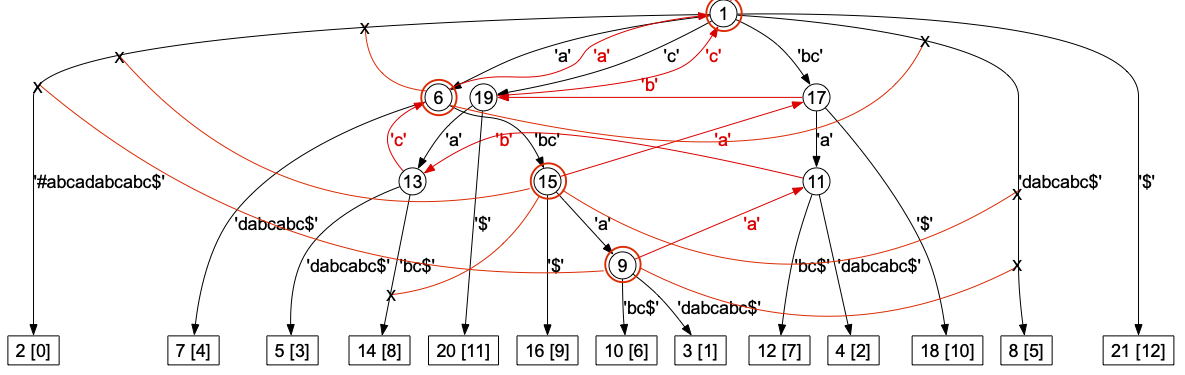
\includegraphics[width=1.00\textwidth]{fig/exp1/fwdstree_org.png}
%% \smallskip
%% \caption{
%%   Illustration of search strategies for maximal repeat enumeration on a string
%%   $S = \mathtt{\#abcadabcabc\$}$ of \cref{tbl:arrays}. 
%%   %S=#abcadabcabc$.
%%   The figure shows the suffix tree (black) and Winer tree (red) of $S$, highlighting maximal repeats with red double circles. Nodes represent right-branching substrings labeled with its SA-range, and edges are labeled with strings (black) or characters (red). Previous methods $\BUSA$ and $\TDBW$ traverse entire subtrees, while our method $\MREnum$ efficiently traverses only relevant red nodes via black edges, significantly reducing the search space.
%% }\label{fig:fwdstree}
%% \end{figure}
%% %%%%%%


%% %%%%%%%%

%% \textbf{Previous work}.\ 
%% %%%%%
%% The current best upperbounds on the runtime of enumerating all distinct  maximal repeats were summarized as the following algorithm schema (see \cref{fig:fwdstree}).
%% The first scheme is abbreviated as \BUSA{} (bottom-up search with the suffix array),  and the best runtime was $O(n)$ time using $O(n)$ words of space based on $SA$, $ISA$, and the RMQ structure on $LCP$, shown by Narisawa, Inenaga, Bannai, and Takeda~\cite{narisawa2007efficient}. 
%% The second scheme is abbreviated as \TDBW{} (top-down search with the Burrows-Wheeler Transformation/BWT), and the runtime was $O(n \log\sigma)$ time using $O(n/\log_\sigma n)$ words of space based on the Wavelet tree on $BWT$, shown by Beller, Berger, and Ohlebusch~\cite{beller:berger2012space:efficient:bbo}.
%% %%where $ISA$ is the inverse $SA$, and $LCP$ is the longest common prefix array of the string.
%% After these seminal work with \textit{uncompressed indexes}~\cite{narisawa2007efficient,beller:berger2012space:efficient:bbo}, there have been a few recent researches on repetition-aware enumeration of maximal repeats with \textit{compressed indexes}~\cite{belazzougui2020linear,nishimoto:cpm2021enum}. For example, Nishimoto and Tabei~\cite{nishimoto:cpm2021enum} have nicely reduced the space to $O(r(S))$ with polylogarithmic factor retaining $O(n)$ time based on a variant of the \textit{$r$-index}. However, to the best of our knowledge, there have been no results that simutaneously achieve sublinear space and time sensitive to repetition parameters including $r(S), z(S)$, or $e_R(S)$. 


%% %%%%%%% tblnew.tex
%% %%% tabnew.tex
%% %\centering
%% \begin{table}[t]
%%   \caption{%
%%     Summary of the time and space of the previous and proposed algorithms for enumeration of all distinct maximal repeats in a string $S$ of length $n$,
%%     %of maximal repeats,
%%     %% where $\sigma$ is the alphabet size,
%%     %% $r$ is the number of BWT runs,
%%     %% $e_R$ is the number of right-extensions,
%%     %% %of maximal repeats,
%%     where
%%     $\sigma$, $r$, and $e_R$ are the numbers of 
%%     characters, BWT runs, and right-extensions, respectively, 
%%     $\delta$ is the substring complexity of $S$.
%%     See \cref{sec:prelim:ds:array} for abbreviations in column \textit{Data structure}, and BU/TD and SA/BW indicate bottom-up/top-down search and SA/BWT arrays, respectively, in \textit{Scheme}.
%% }\label{table:summary:new}
%% %%%% 
%% \medskip
%% \begin{minipage}{\textwidth}
%% %\hspace{-1.2em}
%% \begin{tabular}{%
%% p{.0em}%1margin
%% p{7.6em}%2algo
%% p{10.0em}%3underlying
%% >{\centering}p{7em}%5time
%% %>{\centering}p{8.5em}%6indexspace
%% >{\centering}p{8.5em}%%6indexspace
%% p{3.0em}%4type
%% %c%7dammy
%% %>{}p{4.9em}%7dammy
%% }\toprule
%%   & Algorithm
%%   & Data Structure	
%%   %% & Underlying\break Structure	
%% %% & Index Space
%% & Space (words)
%% & Enum.~Time 
%% & Scheme \\
%% %%%%
%% \midrule 
%% %% \multicolumn{6}{l}{Existing array-based algorithms} \\
%% & Narisawa~\cite{narisawa2007efficient}	&
%% \textsc{Sa,\,Isa,\,Txt,\,Lcp}\cite{manber:myers1993suffixarrays} & $O(n)$	& $O(n)$ & \BUSA{} 	 \\
%% %% & Narisawa~\cite{narisawa2007efficient}	& SA\cite{manber:myers1993suffixarrays} & $O(n)$	& $O(n)$ & \BUSA{} 	 \\
%% %% & Okanohara+~\cite{okanohara2009text}	& SA\cite{manber:myers1993suffixarrays}\&FM\cite{Ferragina05:FM} & $O(n)$& $O(n\log\sigma)$	 & \bufwd 	 \\
%% & Beller+~\cite{beller:berger2012space:efficient:bbo} 	&
%% \textsc{Bwt,\,Wt}~\cite{Ferragina05:FM}
%% & $O(n/\log_\sigma n)$ & $O(n\log\sigma)$	& \TDBW{} \\
%% & Belazzougui+\cite{belazzougui2015space:unusual} 	&
%% \textsc{Bwt,\,Rdq}~\cite{belazzougui2020linear}
%% & $O(n/\log_\sigma n)$ & $O(n)$	& \TDBW{} 	 \\
%% %% & Belazzougui+\cite{belazzougui2020linear} 	& Belazzougui+\cite{belazzougui2020linear} & $O(n)$ & $O(n)$	& \TDBW{} 	 \\
%% %% & Belazzougui+\cite{belazzougui2020linear} 	& Belazzougui+\cite{belazzougui2020linear} & $O(n\log n\log\sigma)$ & $O(n)$	& \TDBW{} 	 \\
%% & Nishimoto+~\cite{nishimoto:cpm2021enum} 	& Gagie+~\cite{gagie:navarro:prezza2020fully} & $O(r\log({\frac n r})\log n)$ & $O(n\polylog n)$ & \TDBW{} 	 \\
%% %%%%%
%% %% \multicolumn{6}{l}{Proposed algorithms} \\
%% \\
%% & [This paper]	&
%% \makebox[11em][l]{\textsc{Sa,\,Isa,\,Txt,\,Rmq$_\textsc{LCP}$}\!\cite{manber:myers1993suffixarrays}}
%%  & $O(n)$ & $O(e_R)$	& \MREnum	 \\
%% %% & [This paper]	& SA\cite{manber:myers1993suffixarrays} & $O(n)$ & $O(e_R)$	& \MREnum	 \\
%% & [This paper]   	& Gagie+~\cite{gagie:navarro:prezza2020fully}	 	& $O(r\log({\frac n r})\log n)$ & $O(e_R \log({\frac n r}))$& \MREnum \\
%% & [This paper]   	& $\delta$-SA~\cite{kempa:kociumaka2023collapsing}  & $O(\delta\log({\frac n \delta}) \log n)$	& $O(e_R \log^{4+\eps}(n))$	 & \MREnum  \\
%% \bottomrule
%% \end{tabular}
%% \end{minipage}
%% \end{table}
%% %%%%%%%

%% %% In particular, we are interested in the complexity of enumerating maximal repeats for highly-repetitive strings, in terms of repetition measures, which take smaler values than the length $n$ of a string. For instance, collections of human genome sequences with small pertabations and Wikipedia documents with edit history are examples of highly-repetitive strings. In highly repetitive strings, a number of measures of repetition growing sublinearly in the length of the string. Particularly, we focus on the repetition measure $e_R(S)$ associated to maximal repeats, introduced by Belazzougui \textit{et al.}~\cite{belazzougui:cunial:gagie:prezza:raffinot2015composite} in 2015, where $e_R(S)$ is the number of right-extensions of maximal repeats in a string~$S$. It is shown by~\cite{belazzougui:cunial:gagie:prezza:raffinot2015composite} that the measure $e_R$ is lowerbounded by other well-known repetition measures $r(S)$ and $z(S)$, the number of runs in the BWT and the number of LZ-phrases of $S$, respectively. 

%% %In this paper, we prove the following theorem.
%% %% To overcome this problem, we propose a simple and faster algorithm with a novel search strategy, which has not been examined so far by the previous work~\cite{narisawa2007efficient,beller:berger2012space:efficient:bbo,belazzougui2020linear,nishimoto:cpm2021enum}.  
%% %% We prove the following theorem.
%% %% To overcome this problem, we propose a simple and faster algorithm scheme, abbreviated \MREnum (top-down search with the suffix array), with a novel search strategy, which has not been examined so far by the previous work~\cite{narisawa2007efficient,beller:berger2012space:efficient:bbo,belazzougui2020linear,nishimoto:cpm2021enum}.  

%% \textbf{Goal of research and main results}.\ 
%% %%%%%
%% To overcome this problem, we propose a novel search scheme, abbreviated as \MREnum{} (top-down search with the suffix array), suitable for simple and faster algorithms, which has not been examined so far by the previous work~\cite{narisawa2007efficient,beller:berger2012space:efficient:bbo,belazzougui2020linear,nishimoto:cpm2021enum}.  
%% We prove the following theorem.

%% %% \begin{trivlist}\item[] \textbf{\cref{thm:algo:main}}
%% %%   Let $S$ be a string of length $n$ over an alphabet of $\sigma\ge 2$ symbols.  We assume any data structure that stores $S$ in $s_\fn{acc}(n)$ words of space supporting (i) access to $SA[i]$ and $ISA[i]$, and (ii) $RMQ_{LCP}(L, R)$ on $LCP$ in $t_\fn{acc}(n)$ worst-case time.
%% %% Then, all of distinct maximal repeats in $S$ can be enumerated in $O(e_R\cdot t_\fn{acc}(n))$ time and $O(\sigma^2 \log e_R)$ words of working space, where $\mu$ is the number of distinct maximal repeats in $S$ and  $e_R$ is the number of the right-extensions of maximal repeats such that $\mu \le e_R \le n$. 
%% %% \end{trivlist}

%% \begin{theorem}[main result]\label{thm:algo:main}
%%   Let $S$ be a string of length $n$ over an alphabet of $\sigma\ge 2$ symbols.
%%   We assume any data structure that stores $S$ in $s_\fn{acc}(n)$ words of space supporting (i) access to $SA[i], ISA[i]$, and $S[i]$, and (ii) $RMQ_{LCP}(L, R)$ on $LCP$ in $t_\fn{acc}(n)$ worst-case time.
%% Then, all of distinct maximal repeats in $S$ can be enumerated in $O(e_R\cdot t_\fn{acc}(n))$ time and $O(\sigma^2 \log e_R)$ words of working space, where $\mu$ is the number of distinct maximal repeats in $S$ and  $e_R$ is the number of their right-extensions such that $\mu \le e_R \le n$. 
%% \end{theorem}

%% By substituting different SA index for \cref{thm:algo:main} above, we obtain a variety of enumeration algorithms for distinct maximal repeats with different time and space trade-offs.
%% In \cref{table:summary:new}, we show the summary of results. 
%% %% 
%% Firstly, we observe the case with the uncompressed SA index of Manber and Myers~\cite{manber:myers1993suffixarrays}, and the RMQ structure $RMQ_{LCP}$ on $LCP$ by Bender and Colton~\cite{bender:colton2000thelcaproblem}. 

%% \begin{theorem}\label{thm:algo:uncompressed:sa}
%%   All distinct maximal repeats in a string $S$ of length $n$ can be enumerated in $O(e_R)$ time and $O(\sigma^2 \log n)$ working space based on $SA, ISA, S$, and $RMQ_{LCP}$ using $O(n)$ words of space. 
%% \end{theorem}

%% Secondly, we observe the cases with the repetition-aware, compressed SA indexes, namely,
%% the \textit{$r$-index} with $O(r\polylog(n))$ space by Gagie \textit{et al.}~\cite{gagie:navarro:prezza2020fully}, and
%% the \textit{$\delta$-spaced SA index} with $O(\delta\polylog(n))$ space by Kempa and Kociumaka~\cite{kempa:kociumaka2023collapsing}, where $\delta \le r \le e_R$ (see \cite{kociumaka:navarro:olivares2024near:delta:optimal,kempa2018roots,belazzougui:cunial:gagie:prezza:raffinot2015composite}).
%% Then, we obtain enumeration algorithms with $O(e_R\polylog(n))$ runtime and space simultaneously shown in the last two lines of \cref{table:summary:new} (\cref{thm:applications}, \ref{item:result:bidirect:index}--\ref{item:result:compressed:delta:index}). 
%% If $e_R = o(n/\log^c n)$ for $c\ge 1$ and $c\ge 4+\eps$, respectively, for hightly-repetitive strings (e.g., Fibonacci or Thue-Morse words~\cite{radoszewski:rytter2012structure:cdawg:thuemorse}), these results yield the first sublinear time and space MR enumeration. 


%% \textbf{Contributions}.\ 
%% %%%%%
%% In this paper, we presented a simple and modular algorithm for enumerating all distinct maximal repeats by using $SA$ and associated auxiliary structures as black box.
%% Technically, the key to our results with time and space complexities that are  sensitive to the repetitiveness measure $e_R$ is a simple and modular algorithm with a novel search strategy (see \cref{fig:fwdstree}), which has not been used before for this problem. 
%% Overall, this work presents the first sublinear, repetitiveness-aware algorithms for highly repetitive strings.

%% %% To overcome the difficulties of the previous approaches, we propose a simple and faster algorithm with a novel search strategy, which has not been examined so far by the previous work~\cite{narisawa2007efficient,beller:berger2012space:efficient:bbo,belazzougui2020linear,nishimoto:cpm2021enum}

%% %% \begin{toappendix}
%% %% We discuss the following applications. 
%% %% In addition to maximal repeats, much attention has been paid to other string patterns in bioinformatics such as minimal absent words (MAWs)~\cite{barton2014linear}, minimal unique substrings (MUSs)~\cite{ilie2011minimum}, and their generalization called minimal rare words (MRWs)~\cite{belazzougui2015space:unusual}. We also focus on these string patterns because they are closely related to maximal repeats~\cite{inenaga2024computing}.
%% %% For applications, our algorithm significantly improves the running times of the previous $O(n)$-time algorithms~\cite{barton2014linear,ilie2011minimum,belazzougui2015space:unusual} based on the suffix array $SA$ with auxiliary structures, for sequence patterns including MAWs, MUSs, and MRWs related to maximal repeats. We also discuss application of our algorithm to faster construction of the CDAWG string index with $SA$. 
%% %% \end{toappendix}

\textbf{Organization of this paper}.\ 
%%%%%
\cref{sec:prelim} introduces basic notions and definitions, necessary to the rest of this paper. 
%% \cref{sec:prev} gives a brief review on the previous approaches in maximal repeats enumeration.
In \cref{sec:mrep} and \cref{sec:algo}, we first present a basic algorithm for enumerating the set $\MR(S)$ of all of $occ$ maximal repeats of a string $S$ over alphabet $\Sigma$ can be enumerated in $O(e_R + occ)$ time and $O(e_L  + |\Sigma|^2 \log n)$ working space, where $n$ is the length of $S$. 
In \cref{sec:mrw}, we extend the basic algorithm to afoementioned classes of unusual words, and show that the set of all patterns of a string $S$ within any of these classes can be enumerated in $O(e_L + e_R + occ)$ time, and give its correctness and computational complexity.
In \cref{sec:conc}, we conclude. 


%% prelim.tex
\section{Preliminaries}
\label{sec:prelim}
%%%%

\subsection{Basics}
We begin with basic definitions and notation following~\cite{charalampopoulos2018extended,barton2014linear,ilie2011minimum,belazzougui2015space:unusual}.
For any integers $i\le j$, we denote by $i..j$ or $[i..j]$ the \textit{discrete interval} $\set{i, i+1, \dots, j}$. For a set $A$, we denote by $|A|$ the \textit{cardinality} of $A$, by $A^*$ and $A^+$ the \textit{sets of all finite sequences} of length $\ge 0$ and length $\ge 1$ over $A$, respectively.
We assume the \textit{unit-cost RAM model} with machine word size $w = \floor{\log n}$ equipped with the standard Boolean and arithmetic operations over integers, where $n$ is an input size~\cite{cormen2009introduction}.

%%%% Strings
\subsection{Strings and factors}
Let $S = S[1]\dots S[n] \in \Sigma^n$ be a \textit{string} (or a \textit{word}) \textit{of length} $n = |S|$ over a finite \textit{alphabet} $\Sigma$ of size $\sigma$. In particular, we consider the case of an \textit{integer alphabet} $\Sigma = \set{0,1,\dots, \sigma - 1} \subseteq \set{1, \dots, n}$. We define $\Sigma(S)$ to be the alphabet of $S$. 
We often write $S[1..|S|]$ for $S$ to emphasize the indexing of $S$, meaning $S: 1..|S| \to \Sigma$. 
For two strings $x[1..m]$ and $y[1..n]$, we denote the \textit{concatenation} of $x$ and $y$ by $(x\cdot y)[1..m+n] = x[1]\dots x[m]\cdot y[1]\dots y[n]$.
For positions $i\le j$ in $S$, we denote by $S[i..j]$ the \textit{factor} (or a \textit{substring}) of $S$ that starts and ends at positions $i$ and $j$, respectively, and by $\eps$ the \textit{empty word} of length $0$. A (non-empty) prefix (resp.~a suffix) of $S$ is a factor of the form $S[1..i]$ (resp.~$S[i..n]$) for some $\btw i1n$. A factor $u$ of a string $w$ is \textit{proper} if $u\not= w$. In what follows, we denote by $\Fac(S)$ and $\Pref(S)$ the \textit{sets of all factors} and \textit{all prefixes} of a string $S$, respectively. 

%%%% Convention
Throughout this paper, we assume an \textit{input string} $S = S[1..n]$ of length $n\ge 1$ over an alphabet $\Sigma$ is given to our algorithms. For convention, we assume an extended alphabet $\hat\Sigma = \Sigma\cup\set{\sharp, \daller}$, where $\#, \daller \not \in \Sigma$. Then, we define an \textit{extended string} $\hat S[0..n+1] = \hat S[0]\cdot S[1..n]\cdot \hat S[n+1]$  over $\hat \Sigma$ of length $n+2$, whose index starts from $0$ by prepending and appending special endmarkers $\hat S[0] = \sharp$ and $\hat S[n+1] = \daller$, respectively. 
%% Under this convention, we formulate classes of patterns in terms of $\hat S$ rather than an input $S$.
%% 
A position $p \in 1..|S|$ is an occurrence of a word $w$ in $S$, if $w = S[p..p+|w|-1]$ holds. Then, we say that $w$ \textit{occurs in} a string $S$ at start position $p$ or end position $q = p + |w| - 1$. 
We denote by $\spos(w)$ and $\epos(w)$ the sets of all start positions and all end positions of $w$ in $S$, respectively. 
We define the number of occurrences of $w$ by $\occ(w) := |\spos(w)| = |\epos(w)|$. 

\subsection{unusual words}
\label{sec:unusual}
%% 
We introduce classes of unusual words of a string $S$.
A string $w \in \Sigma^*$ is \textit{trivial} if $|w| = 1$, i.e., $w = c$ for some letter $c$ in $\Sigma$, and \textit{non-trivial} otherwise.
We can easily see that any non-tivial string $w$ has length two and has the form $w = aub$ for some letter $a, b \in \hat\Sigma$ and a possibly string $u \in \Sigma^*$. Throughout, we assume $|\Sigma(S)|\ge 2$ and consider only non-trivial unusual words.
Let $S = S[1..n] \in \Sigma^n$ be a string over alphabet $\Sigma$.
For convention, we assume virtual extended string $\hat S[0..n+1] = \# S\daller \in \hat\Sigma^{n+2}$ obtained from $S$ by prepending and appending endmarkers, where $S[0] = \#$ and $S[n+1] = \daller$.

%% %%%%
%% \mysubsubsection{Classes of unusual words of a string} 
%% We introduce classes of unusual words of a string $S$. A string $w \in \Sigma^*$ is \textit{trivial} if $|w| = 1$, i.e., $w = c$ for some letter $c$ in $\Sigma$, and \textit{non-trivial} otherwise. We remark that clearly, non-tivial string $w$ has length three and has the form $w = aub$ for some letter $a, b \in \hat\Sigma$ and a non-empty string $u \in \Sigma^+$. Throughout, we consider only non-trivial unusual words.

%% %%%
%% %Ilie and Smyth~\cite{ilie2011minimum} initiated the study of
%% A \textit{minimal unique substrings} (MUSs) of a string $S$, studied by Ilie and Smyth~\cite{ilie2011minimum}, is a non-trivial string $w$ that has unique occurrence in $S$, and any proper factor has more than one occurrences in $S$. 
%% That is, a MUS of $S$ is a string $w = a u b$ with $a, b\in \hat\Sigma$ and $u \in \Sigma^+$ such that
%% \begin{enumerate*}[(i)]
%% \item $\Occ(w) = 1$; and 
%% \item $\Occ(au) \ge 2$ and $\Occ(ub) \ge 2$. 
%% \end{enumerate*}
%% We denote by $\MAW(S)$ and $\MUS(S)$ the sets of all MAWs and all MUSs of a string $S$, respectively. 

%% %%% 
%% The class of \textit{minimal rare words} was introduced by Belazzougui and Cunial~\cite{belazzougui2015space:unusual}, whose abstracted the properties of unusual words with statistical surprise studied by Apostolico, Bock, Lonardi, and Xu~\cite{apostolico2000efficient}. 
%% For every $k\ge 0$, a \textit{$k$-minimal rare word} ($k$-MRW) of a string $S$ is a non-trivial string $w$ that occurs in $S$ exactly $k$ times, and any proper factor occurs in $S$ less frequently (see \cite{belazzougui2015space:unusual}). That is, a $k$-MRW of $S$ is a string $w = a u b$ with $a, b\in \hat\Sigma$ and $u \in \Sigma^+$ such that
%% \begin{enumerate*}[(i)]
%% \item $\Occ(w) = k$; and 
%% \item $\Occ(au) \ge k+1$ and $\Occ(ub) \ge k+1$. 
%% \end{enumerate*}
%% We denote by $\MRW_k(S)$ and $\MRW(S) = \bigcup_{k\ge 0} \MRW_k(S)$ the sets of all $k$-MRWs and all MRWs of a string $S$, respectively. 

%% %%%% 


%% \subsection{Texts, substrings, prefixes, and suffixes}
%% %%%%
%% We assume the word RAM model with machine word size $w = \floor{\log n}$ with input size $n$~\cite{navarro2016cds:book}, where space is always measured in machine \textit{words}, not \textit{bits}. 
%% For any integers $i\le j$, we define intervals $[i]=\set{1,\dots,i}$ and $[i..j] = \set{i, i+1, \dots, j}$.

%% Let $\Sigma$ be an alphabet of $\sigma\ge 2$ characters. We denote by $\eps$ the \textit{empty string} of length $0$, and by $\Sigma^*$ the set of all strings of length $\ge 0$. 
%% Throughout this paper, as input, we always assume a fixed string $S[1..n] = S[1]\dots S[n] \in \Sigma^*$ of length $|S| = n$ over $\Sigma$, called a \textit{text}, where an index starts from $1$. The string is terminated by a special endmarker $S[n]=\daller$, which do not appear elsewhere in $S$, and are smaller than any other characters. $S\rev$ denotes the \textit{reverse} of $S$, i.e., $S\rev = S[n]\dots S[1]$. 
%% If $S = XYZ$ for some strings $X, Y, Z \in \Sigma^*$, we call $X, Y$, and $Z$ a \textit{prefix}, a \textit{substring} and a \textit{suffix} of $S$, respectively.
%% For $1\le p \le q\le n$, $S[p..q]$ denotes the substring of $S$ starting from position $p$ and ends at $q$. Then, $p$ and $q$ are called the \textit{start-position} and \textit{end-position} of $W$.
%% For any string $W \in \Sigma^*$, $\spos[S](W)$, $\epos[S](W)$, and $\occ[S](W) = |\spos[S](W)| = |\epos[S](W)|$  denote the set of all start-positions, the set of all end-positions, and the number of occurrences of $W$ in $S$, respectively.
%% In what follows, we will omit the subscript $S$ if it is clear from context.


%% %% %%%%%%
%% %% %% size: n=12
\begin{table}[t]
\caption{
  The set of lexicographically ordered suffixes of a string \texttt{abcadabcabc\daller} of length $n=13$, where $\# < \daller < a < b < c < d$ and the index starts from $0$. 
}
\ttfamily
\centering 
\begin{tabular}{wc{2.5em}wc{2.5em}wc{2.5em}wc{2.5em}lcccc}
%% \hline
\toprule
rank	& SA	& BWT	& LCP		& suffix	\\
\midrule
0	& 0	& \$	& 0		& \#abcadabcabc\$	\\
1	& 12	& c	& 0		& \$	\\
2	& 9	& c	& 0		& abc\$	\\
3	& 6	& d	& 3		& abcabc\$	\\
4	& 1	& \#	& 4		& abcadabcabc\$	\\
5	& 4	& c	& 1		& adabcabc\$	\\
6	& 10	& a	& 0		& bc\$	\\
7	& 7	& a	& 2		& bcabc\$	\\
8	& 2	& a	& 3		& bcadabcabc\$	\\
9	& 11	& b	& 0		& c\$	\\
10	& 8	& b	& 1		& cabc\$	\\
11	& 3	& b	& 2		& cadabcabc\$	\\
12	& 5	& a	& 0		& dabcabc\$	\\
\bottomrule
\end{tabular}
\end{table}


%% %% size: n=12
%% \begin{table}[t]
%% \caption{
%%   An example of the rank, suffix, inverse suffix, and Burrows-Wheeler Transformation (BWT), and longest common prefix arrays, and the set of lexicographically ordered suffixes of a string \texttt{abcadabcabc\daller} of length $n=13$, where $\# < \daller < a < b < c < d$ and the index starts from $0$. 
%% }\label{tbl:arrays}
%% %% \small 
%% \ttfamily
%% \renewcommand{\arraystretch}{.8}
%% \centering
%% \smallskip
%% \begin{tabular}{wc{2.5em}wc{2.5em}wc{2.5em}wc{2.5em}lcccc}
%% %% \hline
%% \toprule
%% rank	& SA	& BWT	& LCP		& suffix	\\
%% %% index from one 
%% %% \midrule
%% %% 1	& 1	& \$	& 0		& \#abcadabcabc\$	\\
%% %% 2	& 13	& c	& 0		& \$	\\
%% %% 3	& 10	& c	& 0		& abc\$	\\
%% %% 4	& 7	& d	& 3		& abcabc\$	\\
%% %% 5	& 2	& \#	& 4		& abcadabcabc\$	\\
%% %% 6	& 5	& c	& 1		& adabcabc\$	\\
%% %% 7	& 11	& a	& 0		& bc\$	\\
%% %% 8	& 8	& a	& 2		& bcabc\$	\\
%% %% 9	& 3	& a	& 3		& bcadabcabc\$	\\
%% %% 10	& 12	& b	& 0		& c\$	\\
%% %% 11	& 9	& b	& 1		& cabc\$	\\
%% %% 12	& 4	& b	& 2		& cadabcabc\$	\\
%% %% 13	& 6	& a	& 0		& dabcabc\$	\\
%% %% \bottomrule
%% %%
%% %% index from zero
%% \midrule
%% 0	& 0	& \$	& 0		& \#abcadabcabc\$	\\
%% 1	& 12	& c	& 0		& \$	\\
%% 2	& 9	& c	& 0		& abc\$	\\
%% 3	& 6	& d	& 3		& abcabc\$	\\
%% 4	& 1	& \#	& 4		& abcadabcabc\$	\\
%% 5	& 4	& c	& 1		& adabcabc\$	\\
%% 6	& 10	& a	& 0		& bc\$	\\
%% 7	& 7	& a	& 2		& bcabc\$	\\
%% 8	& 2	& a	& 3		& bcadabcabc\$	\\
%% 9	& 11	& b	& 0		& c\$	\\
%% 10	& 8	& b	& 1		& cabc\$	\\
%% 11	& 3	& b	& 2		& cadabcabc\$	\\
%% 12	& 5	& a	& 0		& dabcabc\$	\\
%% \bottomrule
%% \end{tabular}
%% \end{table}
%% %%%%%%%%%%


%%\subsection{Array-like text indexing data structures}
%%\label{sec:prelim:ds:array}
%%%%%%%%%%5
%% Let $S = S[1..n] \in \Sigma^n$ be a string of length $n$ (denoted \textsc{Txt}) throughout.
%% We assume that the reader is familier with fundamental text indexing data structures such as the suffix tree. Below, we introduce basic text indexing array structures.  (See text books, e.g., Gusfield~\cite{gusfield1997book:stree} and Crochemore and Rytter~\cite{crochemore2002jewels} for the suffix tree and the CDAWG, and Navarro~\cite{navarro2016cds:book} for compact array-like text indexing data structures.) 


%%%%%%
\begin{figure}[t]
\centering  
\includegraphics[width=0.70\textwidth]{fig1.pdf}
\vspace{.5\baselineskip}
\caption{An example of indexing arrays of a string $S[1..10] = aabaababb\daller$ of length $n = 10$ over alphabet $\Sigma = \set{a, b}$, whose index starts at $0$, where the left endmarker $S[0]=\#$ and the related suffixes are omitted. 
  Inside and to the right of the panel for sorted suffixes, each bold rectangle $R = [i..j]\times [0..\ell-1]$ and square bracket
indicate a rich representation $(i..j, \ell)$ of a repeat of $S$ and 
the associated SA-interval $i..j$, respectively. 
%% In the panel for sorted suffixes, each bold rectangle $R = [i..j]\times [0..\ell-1]$ in the panel indicates a rich representation $(i..j, \ell)$ of a repeat of $S$, while each square bracket indicates the associated SA-interval $i..j$. 
}\label{fig:example:arrays}
\end{figure}
%%%%%%

\subsection{Text indexing arrays}
%%\label{sec:prelim:ds:array}
Let $S[1..n-1]$ be a string of length $n-1$ and $\hat S[1..n] = S\cdot \daller$ be its extended string with endmarker $\daller \not\in \Sigma$. For any position , we denote by $\Suf[p] = S[p..n]$ the suffix of $S$ starting at position $\btw i1n$. 
We introduce a set of arrays for indexing a string as follows (see~\cite{navarro2016cds:book} for details).
We refer to lexicographic ranks as $i, k$ and positions as $p, q$.


The \textit{suffix array} $SA$ and \textit{inverse suffix array} $ISA$~\cite{manber:myers1993suffixarrays} are integer arrays defined as follows. 
The array $SA$ contains all suffixes of $\hat S[1..n]$ sorted in the increasing lexicographic order $<_\lex$ such that 
$S[SA[1]..n]<_\lex \dots <_\lex S[SA[n]..n]$. that is, $SA[k] = p$ means that $p = SA[k]$ is the starting position of the $k$-th rank in $<_\lex$ in $S$. 
Then, $ISA$ represents the inverse function of $SA$ such that $SA[ISA[p]] = p$ for all $p \in [n]$.

In the \textit{rich representation} on $SA$ array (see, e.g.\cite{kasai:lee2001lcp:linear,abouelhoda2004replacing}), we can uniquely encode any factor $w$ of a string $S$ by a triple $\tau = (i, j, \ell)$, denoted by $(i..j, \ell)$, such that
\begin{enumerate*}[(i)]
\item $i..j \subseteq 1..n$ is the SA-interval of $w$, i.e., $SA[i..j] = \Occ(w)$; and  
\item $\ell$ is the length of $w$, i.e., $\ell = |w|\ge 0$. 
\end{enumerate*}
Conversely, the rich representation $\tau = (i, j, \ell)$ can be decoded by the function $\getfactor(i..j, \ell) := S[p..SA[k]+\ell-1]$ using $\SA$ and $S$, where $\btw kij$ can be any rank in $i..j$. 

The \textit{longest common prefix array} $LCP[1..n]$ contains in the $k$-th rank the length of the longest common prefix of adjuscent suffixes $\Suf[SA[k-1]]$ and $\Suf[SA[k]]$ for all $k \in [n]$; We define $LCP[1] = 0$. It can be preprocessed in linear time supporting the \textit{range minima query} $RMQ_{LCP}(i, j)$ that, given $i\le j$, returns the minimum of $\set{\LCP[i], \LCP[i+1], \dots, \LCP[j]}$ in constant time and $O(n)$ space (Bender and Colton~\cite{bender:colton2000thelcaproblem}).
An example is shown in \cref{fig:example:arrays}. 

%%%
The \textit{Burrows-Wheeler Transformation} $\BWT[1..n]$ defines the permutation of a string $S$ by $BWT[k] = S[SA[k]-1]$ for all $k \in [2..n]$; We let $BWT[k] = \daller$ with $SA[k] = 1$~\cite{burrows:wheeler1994blocksorting}. 
%% For any $k \in [n]$, the \textit{LF-mapping} is defined by $LF(k) = ISA[n]$ if $SA[k]=1$ and $LF(k) = ISA[SA[k]-1]$ otherwise.
%%
It can be preprocessed in linear time in the \textit{Wavelet Tree} data structure (by~\cite{grossi2003high}) supporting the \textit{range distinct query} $RDQ_{BWT}(i, j)$ that, given $i\le j$, returns the set of mutually distinct characters in the range $BWT[i..j]$ in $O(\log\sigma)$ time and
linear space. 
%% $O(n/\log_\sigma n)$ space.
All the arrays can be constructed from $S$ in linear time over integer alphabet (see the textbook~\cite{navarro2016cds:book}). 


%% %%%%% 
%% \subsection{A concise representation of a substring}
%% \label{sec:triple}
%% We introduce a concise representation of a substring $W$ of a string $S$ with constant size, called the \textit{rich representation}, or simply a \textit{triple}, as follows~\cite{kasai:lee2001lcp:linear,ohlebusch2013bookbioinfo,belazzougui2015space:unusual}. 
%% Suppose that $SA \in [n]^n$ is the suffix array of $S$. Let $W \in Substr(S)$ be any substring of $S$. We can easily see that all ranks $k\in [1..n]$ whose starting positions $SA[k]$ belong to $\spos(W)$ occupy the contiguous subinterval $[L..R]\subseteq [1..n]$. We call this range $[L..R]$ the \textit{SA-range} of $W$.
%% We define the \textit{triple} for $W$ to be the integer triple $\tau = (L, R, \ell) \in [n]^3$, denoted $([L..R], \ell)$, such that $[L..R]$ is the SA-range of $W$ and $\ell = |W|$ is the length of $W$.
%% Conversely, $\tau$ \textit{defines} $W$ if $W = S[p..p+\ell-1]$ with $p = SA[L]$ is well-defined for some $k \in [L..R]$, and is unique. 
%% %%% 
%% For example, in \cref{tbl:arrays}, the substring $\mathtt{bc}$ has the triple $([7..9], 2)$ since it has the SA-range $[7,9]$ in $SA[1..13]$ and has the length $|W|=2$.


%% %%%% 
%% \mysubsubsection{Maximal repeats}
%% %%%%
%% To realize efficient enumeration of classes of unusual words, we use the class of maximal repeats of a string $S$, defined as follows.
%% Let $S = S[1..n] \in \Sigma^n$ be a string over alphabet $\Sigma$ and $\hat S[0..n+1] = \# S\daller \in \hat\Sigma^{n+2}$ be its extended version with endmarkers.
%% Let $u \in \Sigma+$ be any factor of $\hat S$. Since $\#, \daller \not\in \Sigma$, we see $u \in \Fac(S)$, namely, $u$ is contained in the content $S$.

%% \begin{definition}[maximal repeat]\rm 
%% A string $u \in \Sigma+$ is a \textit{maximal repeat} of $S$ if it satisfies conditions (1) and (2) below: 
%% \begin{enumerate}[(1)]
%% \item $u$ is a factor of $S$, i.e., $u \in \Fac(S)$. 
  
%% \item there exist two start positions $p, q \in \Spos[S](u)\;(p\not= q)$ of $u$ such that
%%   \begin{enumerate}[(i)]
%%   \item $u$ is \textit{left-branching} meaning that the preceding characters are mutually different, i.e., $S[p-1] \not= S[q-1]$, 
%%  and
%%   \item $u$ is \textit{right-branching} meaning that the following characters are mutually different, i.e., $S[p+|u|] \not= S[q+|u|]$. 
%%   \end{enumerate}
%% \end{enumerate}
%% \end{definition}

%% By definition, any maximal repeat $w$ occurs at least twice in $S$, that is, $w$ is a \textit{repeat} in $S$.
%% For later use, we define some notation: $\LSigma(u) \subseteq \Sigma$ (resp.~$\RSigma[](u)$) to be the sets of the preceding characters $S[p-1] \in \hat\Sigma$ (resp.~the following characters $S[p+|u|] \in \hat\Sigma$) by one over all positions $p\in \Spos(u)$ of $u$ in $\hat S$.
%% If it is clear from context, we write $\LSigma[](u)$ and $\RSigma[](u)$ for $\LSigma(u)$ and $\RSigma(u)$ by omitting subscript $\hat S$, respectively. 
%% In this notation, we see that a nonempty string $u$ is a maximal repeat of $S$ if and only if (1) $u \in \Fac(S)$ and (2) $|\LSigma(u)| \ge 2$ and $|\RSigma(u)| \ge 2$.


%% Now, we define the class of maximal repeats. 
%% %%are one of the most fundamental features in a string. 
%% Any subword $W$ of $S$ is called a \textit{repeat} if it occurs at least twice in $S$, namely, $\occ(W) \ge 2$.
%% A repeat $W$ is said to be \textit{left-branching} (resp.~\textit{right-branching}) in $S$ if either 
%% (i) $W$ is a prefix  of $S$ (resp.~a suffix of $S$), or 
%% (ii) there exist a pair of distict characters $a\not= b$ in $\Sigma$ such that $\occ(aW) \ge 1$ and $\occ(bW) \ge 1$ (resp.~$\occ(Wa) \ge 1$ and $\occ(Wb) \ge 1$).
%% A \textit{maximal repeat} is any repeat $W$ in $S$ that is both right-branching and left-branching in $S$. In what follows, $MR(S)$ denotes the set of all maximal repeats in $S$, and $\mu(S) = |MR(S)|$ denotes their number. 

%% A \textit{left-extension} (resp.~a \textit{right-extension}) of a maximal repeat $W \in MR(S)$ is any substring of $S$ in the form $cW$ (resp.~$Wc$) such that $\occ(cW)\ge 1$ for some $c \in \Sigma$. We denote by $e_L(S)$ (resp.~$e_R(S)$) the number of the left-extensions (resp.~right-extensions) in $S$. 
%% For a substring $W$ of $S$, $[W]^S_L = \sete{ U \in Substr(S) \mid \spos(U) = \spos(W) }$ denotes the equivalence class with the representative $W$, and $\rext W$ denotes the unique longest string in $[W]^S_L$. By symmetry, we can define the equivalence class $[W]^S_R$ and the representative $\lext W$  related to $\epos(W)$.
%% We often write, e.g., $e_L$ and $[W]_L$ for $e_L(S)$ and $[W]^S_L$, by omitting $S$. 

%% \begin{remark}
%% Weobserve the following properties: 
%% (i) for any repeat $W$, $\rext W$ is a right-branching repeat, while $\lext W$ is a left-branching repeat in $S$;
%% (ii) the operators $\set{\lext\cdot, \rext\cdot}$ are
%% %associative,
%% commutative and idenpotent.  
%% %the identities $\rext{(\lext W)} = \lext{(\rext W)} =: \mext W$,  $\lext{(\lext W)} = \lext W$, and  $\rext{(\rext W)} = \rext W$. 
%% (iii) a substring $U$ is a maximal repeat if and only if there exists a substring $W$ such that $U = \mext W := \rext{(\lext W)} = \lext{(\rext W)}$.
%% \end{remark}

%% Raffinot~\cite{raffinot2001maximal} found that the set $MR(S)$ coincides to the vertex set of the CDAWG~\cite{blumer1987complete} for a string $S$. 
%% Thus, $e_R$ satisfies $\mu \le e_R \le n$ and $\sigma \le e_R \le n$~\cite{blumer1987complete,raffinot2001maximal}. 
%% Belazzougui~\textit{et al.}~\cite{belazzougui:cunial:gagie:prezza:raffinot2015composite} have focused on $e_R$ as a fundamental repetitiveness measure related to $MR(S)$, and showed that $r \le e_R$ and $z \le e_R$. In general, $e_R = \Theta(n)$, while $e_R$ can be much smaller than $n$ for highly-repetitive strings. Radoszewski et al.~\cite{radoszewski:rytter2012structure:cdawg:thuemorse} showed that $e_R = O(\log n)$ for morphic strings, e.g.~Thue-Morse words.

%%% maw.tex
%% \section{Minimal Absent Words and Maximal Repeats}
\section{Minimal Rare Words and Maximal Repeats}
\label{sec:mrep}

%% We introduce a fundamental concept of maximal repeats of a string $S$, which is useful for realizing efficient enumeration of many kinds of unusual words. Then, we give a characterization of the set $\MRW(S)$ of minimal rare words of a string $S$.
%% 
We introduce classes of unusual words of a string $S$.
A string $w \in \Sigma^*$ is \textit{trivial} if $|w| = 1$, i.e., $w = c$ for some letter $c$ in $\Sigma$, and \textit{non-trivial} otherwise.
We can easily see that any non-tivial string $w$ has length two and has the form $w = aub$ for some letter $a, b \in \hat\Sigma$ and a possibly string $u \in \Sigma^*$. Throughout, we assume $|\Sigma(S)|\ge 2$ and consider only non-trivial unusual words.
Let $S = S[1..n] \in \Sigma^n$ be a string over alphabet $\Sigma$.
For convention, we assume virtual extended string $\hat S[0..n+1] = \# S\daller \in \hat\Sigma^{n+2}$ obtained from $S$ by prepending and appending endmarkers, where $S[0] = \#$ and $S[n+1] = \daller$.

%%%% 
\mysubsubsection{Maximal repeats}
%%%%
Maximal repeats of a string is a fundamental concepts in discovery of unusual words, and introduced as follows.  
A \textit{repeat} of $S$ is any substring $u \in \Sigma^+$ that occurs at least twice in $S$, that is, $u \in \Fac(S)$.
Let $u \in \Sigma+$ be any factor of $\hat S$. Since $\#, \daller \not\in \Sigma$, we see $u \in \Fac(S)$, namely, $u$ is contained in the content $S$.

\begin{definition}[maximal repeat]\rm 
A string $u \in \Sigma+$ is a \textit{maximal repeat} of $S$ if it satisfies the following conditions: 
\begin{enumerate*}[(1)]
\item $u$ is a factor of $S$, i.e., $u \in \Fac(S)$;  
\item there exist two start positions $p, q \in \Spos[S](u)\;(p\not= q)$ of $u$ such that
  \begin{enumerate*}[(i)]
  \item $u$ is \textit{left-branching} meaning that the preceding characters are mutually different, i.e., $S[p-1] \not= S[q-1]$, and
  \item $u$ is \textit{right-branching} meaning that the following characters are mutually different, i.e., $S[p+|u|] \not= S[q+|u|]$. 
  \end{enumerate*}
\end{enumerate*}
\end{definition}

In what follows, $\MR(S)$ denotes the set of all maximal repeats of a string $S$. By definition, any $w$ in $\MR(S)$ correctly occurs at least twice in $S$. 
For later use, we define the \textit{set of left characters} $\LSigma(u) \subseteq \Sigma\cup\set{\#}$ (resp.~\textit{right characters} $\RSigma[](u) \subseteq \Sigma\cup\set{\daller}$) of a factor $u \in \Fac(S)$ to be the sets of all characters $S[p-1] \in \hat\Sigma$ (resp.~$S[p+|u|] \in \hat\Sigma$) preceding (resp.~following) all positions $p\in \Spos(u)$ of $u$ in $\hat S$.
If it is clear from context, we write $\LSigma[](u)$ and $\RSigma[](u)$ by omitting subscript $\hat S$. 
Using this notation, we can redefine a maximal repeat of $S$ to be any nonempty string $u \in \Fac(S)$ with $|\LSigma(u)| \ge 2$ and $|\RSigma(u)| \ge 2$.


%%%
\mysubsubsection{Minimal rare words}
%%%% 
The class of \textit{minimal rare words} was introduced by Belazzougui and Cunial~\cite{belazzougui2015space:unusual}, whose abstracted the properties of unusual words with statistical surprise studied by Apostolico, Bock, Lonardi, and Xu~\cite{apostolico2000efficient}.

\begin{definition}[minimal rare word]\rm 
For every integer $k\ge 0$, a \textit{$k$-minimal rare word} ($k$-MRW) of a string $S$ is a non-trivial string $w$ that occurs in $S$ exactly $k$ times, and any proper factor occurs in $S$ less frequently (see \cite{belazzougui2015space:unusual}). That is, a $k$-MRW of $S$ is a string $w = a u b$ with $a, b\in \hat\Sigma$ and $u \in \Sigma^+$ such that
\begin{enumerate*}[(i)]
\item $\Occ(aub) = k$; and 
\item $\Occ(au) > k$ and $\Occ(ub) > k$. 
\end{enumerate*}
We denote by $\MRW_k(S)$ and $\MRW(S) = \bigcup_{k\ge 0} \MRW_k(S)$ the sets of all $k$-MRWs and all MRWs of a string $S$, respectively.
\end{definition}

 %%%
Ilie and Smyth~\cite{ilie2011minimum} initiated the study of \textit{minimal unique substrings} (MUSs) of a string $S$, studied by Ilie and Smyth~\cite{ilie2011minimum}, is a non-trivial string $w$ that has unique occurrence in $S$, and any proper factor has more than one occurrences in $S$. 
That is, a MUS of $S$ is a string $w = a u b$ with $a, b\in \hat\Sigma$ and $u \in \Sigma^+$ such that
\begin{enumerate*}[(i)]
\item $\Occ(w) = 1$; and 
\item $\Occ(au) \ge 2$ and $\Occ(ub) \ge 2$. 
\end{enumerate*}
We denote by $\MAW(S)$ and $\MUS(S)$ the sets of all MAWs and all MUSs of a string $S$, respectively. 


As an example, the string $S = \texttt{aabaababb}$ has the following five maximal repeats $\tt \eps, a, aaba, ab$, and $\tt b$.
For instance, the factor $bab$ of $S$ is a $1$-minimal rare words since if we put $a = \op{b}, b = \op{b}$, $u = \op{a}$ and $k = 1$, we can check if the condition 
$\Occ(aub)= \Occ(\op{bab})= 1 = k$, 
$\Occ(au) = \Occ(\op{ba}) = 2 \ge k+1$, and 
$\Occ(ub) = \Occ(\op{ab}) = 3 \ge k+1$ hold. 

% of the string $S = \texttt{aabaababb}$ are shown in \cref{fig:example:maw}. 


%% \mysubsubsection[]{Minimal rare words}
%% %%%% 
%% (MRW, for short) of a string $S$ are a class of unusual words, introduced by
%% Belazzougui and Cunial~\cite{belazzougui2015space:unusual}
%% %% Garcia, Pinho, Rodrigues, Bastos, and Ferreira~\cite{garcia2011minimal}.
%% A \textit{MRW} is a non-trivial string $w$ that does not occur in $S$, and any proper factor of $w$ occurs in $S$ as a substring (see \cite{garcia2011minimal}).
%% Precisely, a MRW of $S$ is a string $a u b$ with $a, b\in \hat\Sigma$ and $u \in \Sigma^+$ such that
%% \begin{enumerate*}[(i)]
%% \item $w \not\in \Fac(\hat S)$; and 
%% \item $au, ub \in \Fac(\hat S)$. 
%% \end{enumerate*}

%% \mysubsubsection[]{Minimal absent words}
%% %%%% 
%% %A \textit{minimal absent word} (MRW)
%% of a string $S$ are a class of unusual words, introduced by Garcia, Pinho, Rodrigues, Bastos, and Ferreira~\cite{garcia2011minimal}. A \textit{MRW} is a non-trivial string $w$ that does not occur in $S$, and any proper factor of $w$ occurs in $S$ as a substring (see \cite{garcia2011minimal}).
%% Precisely, a MRW of $S$ is a string $a u b$ with $a, b\in \hat\Sigma$ and $u \in \Sigma^+$ such that
%% \begin{enumerate*}[(i)]
%% \item $w \not\in \Fac(\hat S)$; and 
%% \item $au, ub \in \Fac(\hat S)$. 
%% \end{enumerate*}

%% As an example, the minimal absent words of the string $S = \texttt{aabaababb}$ are shown in \cref{fig:example:maw}. 

%%%%%%
%% \begin{algorithm}[t]
%% \centering  
%% %% \includegraphics[width=0.60\textwidth]{fig/exp1/fig1.pdf}
%% \vspace{.5\baselineskip}
  %% \setlength{\interspacetitleruled}{0pt}%
%% \setlength{\algotitleheightrule}{0pt}%


%% %%%%%%
%% \begin{figure}[t]
%% \centering  
%% %% \includegraphics[width=0.60\textwidth]{fig/exp1/fig1.pdf}
%% \vspace{.5\baselineskip}
%% \caption{An example of minimal absent words of the string $S = \texttt{aabaababb}$. 
%% }\label{fig:example:maw}
%% \end{figure}
%% %%%%%%
%% %%%%%%%%%%%%%%%%%
%% \bgroup
%% {
%%   \setlength{\interspacetitleruled}{0pt}%
%%   \setlength{\algotitleheightrule}{0pt}%  
%%   \begin{algorithm}[h]
%%   %% \caption{Top-down MR-enumeration algorithm with \SA}\label{algo:maxrep:tdfw}
%%   \textbf{Procedure} \MRRec$(\tau_0 = ([L_0..R_0], \ell_0))$:\\
%%   %%\KwGiven{}
%%   %% \KwIn{The triple $\tau_0 = (L_0, R_0, \ell_0)$ for a right-branching substring $X$ of a string.}
%%   %% \KwOut{}
%%   \Begin{
%%       \textbf{output} $\tau_0$
%%       \Comment*{A maximal repeat is found}
%%       \For %(\CM{})
%%            {child $\tau = ([L..R], \ell)$ of the parent $([L_0..R_0], \ell_0)$}{
%%           \Comment{It is ensured that $R - L \ge 1$ and $\tau$ is right-branching}
%%           Decide if $\tau$ is left-branching by $\SA, \ISA$, and $S$ (\cref{lem:leftmaximal:character})\; 
%%           \If {$\tau$ is left-branching}{          
%%             \MRRec$(\tau)$\; 
%%           }
%%         }
%%   }
%%   \end{algorithm}
%% \egroup
%% %%%%%%%%%%%%%%%%%



%%% EOF

%%% mrw.tex
%%% from spire2024 sub

\section{A Modified Algorithm for Minimal Rare Words}
\label{sec:mrw}

%%%%%%%%%%%%%%
%\paragraph{Algorithms for MRW}
In this section, we present a modified algorithm for computing $\MRWK[k]$ with any $k\ge 1$.

\subsection{Definition}
%%%% 
The class of \textit{minimal rare words} was introduced by Belazzougui and Cunial~\cite{belazzougui2015space:unusual}, whose abstracted the properties of unusual words with statistical surprise studied by Apostolico, Bock, Lonardi, and Xu~\cite{apostolico2000efficient}.

\begin{definition}[minimal rare word]\rm 
  For every integer $k\ge 0$,
  a \textit{$k$-minimal rare word with frequency $k$}, or simply 
  a \textit{$k$-minimal rare word} ($k$-MRW), of a string $S$ is a non-trivial string $w$ that occurs in $S$ exactly $k$ times, and any proper factor occurs in $S$ less frequently (see \cite{belazzougui2015space:unusual}). That is, a $k$-MRW of $S$ is a string $w = a u b$ with $a, b\in \hat\Sigma$ and $u \in \Sigma^+$ such that
\begin{enumerate*}[(i)]
\item $\Occ(aub) = k$; and 
\item $\Occ(au) > k$ and $\Occ(ub) > k$. 
\end{enumerate*}
\end{definition}

A $k$-minimal rare word with frequency $k\ge 1$ is called a \textit{positive minimal rare word} (positive MRW) if $k \ge 1$ and a \textit{minimal rare word} (MRW) if $k\ge 0$. 
In what follows, we denote by
$\MRW_k(S)$, 
$\MRW_{+}(S) = \bigcup_{k\ge 1} \MRW_k(S)$, and 
$\MRW(S) = \bigcup_{k\ge 0} \MRW_k(S)$
the sets of
all $k$-MRWs,
all positive MRWs, and
all MRWs
of a string $S$, respectively.

%% We denote by
%% $\MRW_k(S)$ 
%% and $\MRW(S) = \bigcup_{k\ge 0} \MRW_k(S)$ the sets of all $k$-MRWs and all MRWs of a string $S$, respectively.

%% %%% def
%% Ilie and Smyth~\cite{ilie2011minimum} initiated the study of \textit{minimal unique substrings} (MUSs) of a string $S$, studied by Ilie and Smyth~\cite{ilie2011minimum}, is a non-trivial string $w$ that has unique occurrence in $S$, and any proper factor has more than one occurrences in $S$.
%% That is, a MUS of $S$ is a string $w = a u b$ with $a, b\in \hat\Sigma$ and $u \in \Sigma^+$ such that
%% \begin{enumerate*}[(i)]
%% \item $\Occ(w) = 1$; and 
%% \item $\Occ(au) \ge 2$ and $\Occ(ub) \ge 2$. 
%% \end{enumerate*}

%% Garcia, Pinho, Rodrigues, Bastos, and Ferreira~\cite{garcia2011minimal} studied enumeration of minimal absent words in a string $S$.
%% A \textit{minimal absent words} (MAWs) is a non-trivial string $w$ that does not occur in $S$, and any proper factor of $w$ occurs in $S$ as a substring (see \cite{garcia2011minimal}).
%% Precisely, a MAW of $S$ is a string $a u b$ with $a, b\in \hat\Sigma$ and $u \in \Sigma^+$ such that
%% \begin{enumerate*}[(i)]
%% \item $w \not\in \Fac(\hat S)$; and 
%% \item $au, ub \in \Fac(\hat S)$. 
%% \end{enumerate*}

%%% def
Below, we introduce classes of patterns in a string $S$, which are closely related to MRWs. 
%%
Garcia, Pinho, Rodrigues, Bastos, and Ferreira~\cite{garcia2011minimal} studied enumeration of \textit{minimal absent words} (MAWs) in a string $S$, which is a non-trivial string $w$ that does not occur in $S$, and any proper factor of $w$ occurs in $S$ as a substring (see \cite{garcia2011minimal}).
%% Precisely, a MAW of $S$ is a string $a u b$ with $a, b\in \hat\Sigma$ and $u \in \Sigma^+$ such that
%% \begin{enumerate*}[(i)]
%% \item $w \not\in \Fac(\hat S)$; and 
%% \item $au, ub \in \Fac(\hat S)$. 
%% \end{enumerate*}
%% 
Ilie and Smyth~\cite{ilie2011minimum} initiated the study of \textit{minimal unique substrings} (MUSs) of a string $S$, studied by Ilie and Smyth~\cite{ilie2011minimum}, which is a non-trivial string $w$ that has unique occurrence in $S$, and any proper factor has more than one occurrences in $S$.
%% That is, a MUS of $S$ is a string $w = a u b$ with $a, b\in \hat\Sigma$ and $u \in \Sigma^+$ such that
%% \begin{enumerate*}[(i)]
%% \item $\Occ(w) = 1$; and 
%% \item $\Occ(au) \ge 2$ and $\Occ(ub) \ge 2$. 
%% \end{enumerate*}
%% 
%%%
These classes of patterns are formally defined as follows. 

\begin{definition}
  We define the following class of patterns.
  Let $w$ be any string $w = a u b$ with some characters $a, b\in \hat\Sigma$ and non-empty word $u \in \Sigma^+$. 
  \begin{itemize}
  %%
  \item A string $w = a u b$ is a minimal absent word (MAW) of $S$ is a string $a u b$ if 
  \begin{enumerate*}[(i)]
  \item $w \not\in \Fac(\hat S)$; and
  \item $au, ub \in \Fac(\hat S)$.
  \end{enumerate*}

  %% 
  \item A string $w = a u b$ is a minimal unique word (MUS) of $S$ if 
    \begin{enumerate*}[(i)]
    \item $w \in \Fac(\hat S)$; and
    \item $\Occ(au) \ge 2$ and $\Occ(ub) \ge 2$.
    \end{enumerate*}

  %% 
  \item A string $w = a u b$ is an extended bispecial factor (EBF) of $S$ is a string $w = a u b$ if 
    \begin{enumerate*}[(i)]
    \item $w \in \Fac(\hat S)$; and
    \item $cu, ud \in \Fac(\hat S)$
      for some characters $c, d \in \hat\Sigma$. 
    \end{enumerate*}

\end{itemize}
\end{definition}

We denote by $\MAW(S)$, $\MUS(S)$, and $\EBF(S)$ the sets of all MAWs, all MUSs, and all EBFs of a string $S$, respectively.
The following fact follows immediate from the definitions of MUSs and MAWs.

\begin{lemma}[Belazzougui and Cunial~\cite{belazzougui2015space:unusual}, Inenaga et al.~\cite{inenaga2024computing}]
  For any string $S$,
  $\MAW(S) = \MRW_0(S)$ and 
  $\MUS(S) = \MRW_1(S)$. 
\end{lemma}

\begin{example}
  Consider the string $S = \texttt{aabaababb}$ over alphabet $\Sigma = \set{a, b}$.
\begin{itemize}
\item $S$ contains five maximal repeats $\tt \eps, a, aaba, ab$, and $\tt b$.
\item The string $\tt bba$ is an example of a MAW of $S$ since we can see that
$aub = \op{bba} \not\in \Fac(S)$, 
$au = \op{bb} \in \Fac(S)$, and 
  $ub = \op{ba} \in \Fac(S)$ hold
  for $a = \op{b}, u = \op{b}$, and $b = \op{a}$. 
  
\item The string $\tt bab$ is an example of a MUS of $S$
  since
  %% if we put $a = \op{b}, u = \op{a}, b = \op{b}$,
  we can see that 
$\Occ[S](aub)= \Occ[S](\op{bab})= 1$, 
$\Occ[S](au) = \Occ[S](\op{ba}) = 2 > 1$, and 
  $\Occ[S](ub) = \Occ[S](\op{ab}) = 3 > 1$ hold
  for $a = \op{b}, u = \op{a}$, and $b = \op{b}$. 

\item The string $\tt aaba$ is an example of an EBF of $S$
  since we can see that 
$aub = \op{aaba} \in \Fac(S)$, 
$cu = \op{bab} \in \Fac(S)$ for $c = \op{b}$, and 
  $ud = \op{abb} \in \Fac(S)$ for $d = \op{b}$ hold
  for $a = \op{b}, u = \op{ab}$, and $b = \op{a}$. 
  Furthermore, we observe that the frequencies of $aub, au$, and $ub$ satisfy 
  $\Occ[S](aub) = \Occ[S](\op{aaba}) = 1$
  $\Occ[S](au) = \Occ[S](\op{aab}) = 2$, and  
  $\Occ[S](ub) = \Occ[S](\op{aba}) = 2$, respectively.
  Thus, $\tt aaba$ is also a $1$-MRW (i.e., a MUS) of $S$. 
\end{itemize}
\end{example}

From the last example for EBF, one might wonder if any EBF of $S$ is always a positive MRW of $S$. However, it is not true in general.
Actually, we observe that $\EBF(S) \not\subseteq \MRW_{+}(S)$ for some $S$ by the following counter example. Consider the string 
  $S = \tt p\, aaba\, q\, aaba\, r\, cabd\, s$
  over $\Sigma = {\tt a, b, c, d, p, q, r, s}$ and a factor $w = aub = \tt a ab a$ with $a = \op a, u = \op{ab}, b = \op a$.
  Then, $aub$ is an EBF since $\op{aaba} \in \Fac(S)$ and
  $\op{aab, aba, cab, abd} \in \Fac(S)$ with $c = \tt c$ and $d = \tt d$. On the other hand, we see that
  $\Occ[S](\op{aaba}) = \Occ[S](\op{aab}) = \Occ[S](\op{aba}) = 2$.
  Since the frequency of $\op{aaba}$ equals to $\tt aab, aba$, $\op{aaba}$ is not an MRW of $S$.

  On the other hand, we can show that $\MRW_{+}(S) \subseteq \EBF(S)$ as follows. Let $aub$ be any member of $\MRW_k(S)$ with some $k\ge 1$.
  It follows from \cref{lem:posmrw:characterization} that (ii) $|\LSigma[](ub)| \ge 2$. Therefore, we have some character $c \in \Sigma$ with $a \not= c$ such that $c \in \LSigma[](ub)$. This implies that $cub \in \Fac(S)$, and thus, $cu \in \Fac(S)$. By symmetry, it follows from \cref{lem:posmrw:characterization}, (iii) $|\RSigma[](au)| \ge 2$. By similar arguments as above, we have $ud \in \Fac(S)$. Combining above arguments, we have $aub, cu, ud \in \Fac(S)$, and thus, $aub$ is an EBF of $S$.

\begin{lemma}[characterization of $\EBF(S)$]
    \label{lem:characterization:ebf}
For any $a, b \in \Sigma$ and $u\in\Sigma^*$, 
\begin{enumerate*}[(1)]
\item $aub \in \EBF(S)$ if and only if 
\item $u\in\MR(S)$. 
\end{enumerate*}
\end{lemma}

  \begin{proof}
    Let $aub$ be any string satisfying the above assumption. . 
    (1) $\Rightarrow$ (2): Suppose that $aub$ is an EBF of $S$. By definition, $aub, cu, ud \in \Fac(S)$ for some $c, d \in \Sigma$ with $c \not= a$ and $d \not= b$.
    Since $aub\in \Fac(S)$ implies $au, ub\in \Fac(S)$,
    we have both of $au$ and $cu$ with $a\not=c$ are contained in $S$. Terefore, we have $a, c \in \LSigma[S](u)$, and thus, $u$ is left-branching. By symmetry, we also have $b, d \in \RSigma[S](u)$, and thus, $u$ is right-branching. Combining the above arguments, we conclude that $u$ is a maximal repeat of $S$. 
%%% 
    (2) $\Rightarrow$ (1): Suppose that $u \in \MR(S)$. By definition, $u$ is both left- and right-branching factor of $S$, namely,
    $|\LSigma[S](u)| \ge 2$ and $|\RSigma[S](u)| \ge 2$ hold. By assumption, we see that $a \in \LSigma[S](u)$ and $b \in \RSigma[S](u)$. By selecting any pair of characters $c \in \LSigma[S](u)\setminus\set{a}$ and $d \in \RSigma[S](u)\setminus\set{b}$, we have $au, cu, ub, ud \in \Fac(S)$ with $c \not= a$ and $d \not= b$, and thus, $aub$ is an EBF of~$S$. \qed 
  \end{proof}

\begin{remark}
For any string $S$, $\MRW_{+}(S) \subseteq \EBF(S)$. The converse is not true in general. Acturally, $\EBF(S) \not\subseteq \MRW_{+}(S)$ for some string~$S$. 
\end{remark}

%%%%%%
\begin{figure}[t]
\centering  
\includegraphics[width=0.60\textwidth]{fig3mrwproof.pdf}
\vspace{.5\baselineskip}
\caption{
  An example of the parent of a positive MRW $w = aub$ of a string $S$.
  The parent is the longest proper prefix $v = w[1..\ell] = a u_i b_i$ of $w$ that is right-branching in $S = S[1..n]$. 
}\label{fig:mrw:parent}
\end{figure}
%%%%%%

\subsection{Characterization}
%%%% 
We start with a characterization of $\MRWS[\ge k](S) := \bigcup_{k\ge 1}\MRWK[k]$ in maximal repeats in $\MR$. 
Suppose that $|S|\ge 2$ and $|\Sigma(S)|\ge 2$
The next lemma is a slightly modified version of the result shown by Belazzougui and Cunial~\cite{belazzougui2015space:unusual}. For the completeness, we show a sketch of the proof. 

\begin{lemma}[characterization of $\MRW_k(S)$ by Belazzougui and Cunial~\cite{belazzougui2015space:unusual}]\label{lem:posmrw:characterization}
For any $k\ge 0$, any $a, b \in \Sigma$, and $u\in\Sigma^*$, 
\begin{enumerate*}[(1)]
\item $aub \in \MRWK[k]$ if and only if 
\item $u\in\MR(S)$, $|\RSigma[](au)| \ge 2$, $|\LSigma[](ub)| \ge 2$, and $\Occ[](aub) = k$. 
\end{enumerate*}
\end{lemma}

\begin{proof}
  (1) $\Rightarrow$ (2):  Suppose that $aub \in \MRWK[k]$ holds. From defininition, $\Occ[](aub) = k$ follows. By contradiction, suppose that $|\RSigma[](au)| = 1$. If we let $\RSigma[](au) = \set{c}$ for a character $c \in \Sigma$, it follows that $\Occ[](au) = \Occ[](aub) = k$, contradiction. Therefore, we have $|\RSigma[](au)| \ge 2$. Since $|\RSigma[](u)| \ge |\RSigma[](au)| \ge 2$, we see that $u$ is right-branching. By symmetry, we can also show that $|\LSigma[](ub)| \ge 2$, and thus, $u$ is left-branching. Combining the arguments, we conclude that $u \in \MR(S)$.
  %%% 
 (2) $\Rightarrow$ (1):  Suppose that $\Occ[](aub) = k$. 
  If $|\RSigma[](au)| \ge 2$ and character $b$ is contained in $\RSigma[](au)$, then we have $\Occ[](au) > \Occ[](aub) = k$. By symmetry, if $|\RSigma[](au)| \ge 2$, then $\Occ[](ub) > \Occ[](aub) = k$ follows. Combining the above arguments, the claim is proved. 
\qed\end{proof}

\begin{definition}[The parent of a positive MRW]
  \label{def:mrw:parent}
  Given any positive MRW $w = aub$ of $S$, the parent of $w$, is the longest proper prefix
  $\op{parent}_{S}(w)
  := w[1..\ell]
  = a u' b'$
  of $w$ with length $1\le \ell \le |w|-1$ that is right-branching in~$S$, where
  $a = w[1]$, 
  $u' = w[2..\ell-1]$, and 
  $b' = w[\ell]$ (see \cref{fig:mrw:parent}).
  %%
Given any positive MRW $v$ of $S$, if there exists some string $w$ such that $v = \op{parent}_{S}(w)$, then we call $w$ a child of $v$. 
\end{definition}

Let $\mext{\eps}$ be the shortest maximal repeat of $S$. We note that such $\mext{\eps} = \eps$ always exists and unique when $|\Sigma| \ge 2$. 

\begin{lemma}[the parent of a positive MRW]
  \label{lem:posmrw:parent}
  Let $w = aub \in \MRW_+$ be any positive MRW of $S$, with $a, b \in \Sigma$ and $u\not= \mext{\eps} \;(u\in\Sigma^*)$. Then, $v = \op{parent}_{S}(w)$ satisfies the conditions (1)--(3) below: 
\begin{enumerate}[(1)]
\item $v$ is well-defined and unique.
  
\item $v$ is a positive MRW of $S$, that is, $v \in \MRW_+(S)$.
  
  %% \item (wrong) $v$ has a form of $v = a u' b'$, where $u'$ is the longest proper prefix of an MR $u$  of $S$ that is also an MR of $S$, and $a = w[1]$  and $b = w[|u'|+1]$.
  
\item \label{item:posmrw:parent:three}
  There exists a character $c \in \Sigma$ that recovers $w$ from $v$ by $w = \rext{(vc)}$. Moreover, such a character $c$ is unique, that is, $w \not= \rext{(vd)}$ for any $d \in \Sigma$ with $d\not= c$. 
\end{enumerate}
\end{lemma}


\begin{lemma}[Conjecture; children of a positive MRW]
  \label{lem:posmrw:child}
  Let $v = aub$ be any positive MRW of $S$.
  For the unique maximal right-extension of $v$, $au' := \rext{v} = \rext{(aub)}$, and any character $b' \in \RSigma[S](au')$, the string $w = a u' b'$ satisfies the conditions (1)--(3) below: 
  \begin{enumerate}[(1)]
  \item $w \in \Fac(S)$. 
  \item $w$ is a positive MRW of $S$.
  \item $w$ is a child of $v$, i.e., $v = \op{parent}_S(w)$ holds. 
  \end{enumerate}
\end{lemma}


%% From \cref{item:posmrw:parent:three} of \cref{lem:posmrw:parent}, we define a child


%%%%%%%%%%%%%%%%%%%%%%%%%%%%
\begin{algorithm}[t]
  \caption{A fragment of the code for a modified algorithm for enumerating the set $\MRW_+(S)$ of all minimal rare words of a string $S$ over alphabet $\Sigma$.
    We remark that the modified algorithm uses $\BWT(S)$ with $RMQ$ and $WT$ in addition to $\SA(S), \ISA(S)$, $S$, and $\LCP(S)$ with $RMQ$. 
}\label{fig:example:mrw:subcode}
%%%\medskip
  \KwInput{
    A triple $\pair{i..j, \ell} \in \RREP$ for a MR $u$,
    a monotone constraint $\Theta \subseteq \Sigma^*$, and 
    a set $Words \subseteq \RREP$. 
  }
  \Begin{
      $Children \gets \GenChildren(i..j, \ell, Children)$\; 
      \For (\comblk{the triple for $ub$})
           {each child $(b, \pair{i_b..j_b, \ell_b}) \in Children$
           }{
        \Comment{Modified 1: Check whether $|\LSigma[S](ub)|\ge 2$}
        $L_b \gets \ColoredRange(i_b, j_b)$
        \Comment*{$L_b = \LSigma[S](ub)$}
        \If (\comblk{Case: $|\LSigma[S](ub)|\ge 2$})
            { $|L_b|\ge 2$ }{
          %% $L_b \gets \ColoredRange(i_b, j_b)$\; 
              \For (\comblk{
                %$k_{ab} = |\Occ[](aub)|$  for
                $a \in \LSigma[S](ub)$
                implies $aub \in \Fac(S)$
              })
                   {each $a \in L_b$
                   }{
                 \Comment{Modified 2: Check whether $|\RSigma[S](au)|\ge 2$}
                 \Comment{Compute the triple $\pair{i_a..j_a, \ell_a}$ for $au$}
                 $i_{a}\gets LF_{BWT,WT}(i)$;
                 $j_{a} \gets LF_{BWT,WT}(j)$;
                 $\ell_{a} \gets \ell + 1$\; 
                 \If (\comblk{Case: $|\RSigma[S](au)|\ge 2$})
                     {
                       $RMQ_{LCP}(i_a+1, j_a) = \ell_a$
                     }{
                   \Comment{Output the triple $\pair{i_{ab}..j_{ab}, \ell_{ab}}$ for $aub$}
                   $i_{ab}\gets LF_{BWT,WT}(i_b)$;
                   $j_{ab} \gets LF_{BWT,WT}(j_b)$;
                   $\ell_{ab} \gets \ell + 2$\;
                   $Words.\append(\pair{i_{ab}..j_{ab}, \ell_{ab}})$\;
                 }
               }
               $Words \gets \MRRec(\pair{i_b..j_b, \ell_b}, \Theta, Words)$\;
        } %% if
      } %% for
    }%% Begin
\end{algorithm}
%%%%%%%%%%%%%%%%%%%%%%%%%%%%

\subsection{Algorithm}
%%%% 
Based on \cref{lem:posmrw:characterization}, we will modify the basic algoritm shown in Algorithms~\ref{fig:example:mrep:main} and~\ref{fig:example:mrep:sub} that enumerates the set $\MRW_+(S)$ of all positive MRWs of $S$. In Algorithm~\ref{fig:example:mrw:subcode}, we show a fragment of codes that we substitute for the for-loop from \ref{line:recmr:for:begin} to \ref{line:recmr:for:end} of the recursive subprocedure $\MRRec$ in Algorithm~\ref{fig:example:mrep:sub}.

  Combining \cref{lem:posmrw:characterization} and  \cref{lem:posmrw:parent}, we can show the correctness and computational complexity of the modified algorithm as follows. 

\begin{theorem}[Output-sensitive enumeration of $\MRW_+(S)$]\label{thm:algo:mrw}
  For any any string $S$ of length $n$ over an integer alphabet $\Sigma$ with $|\Sigma| \ge 2$, all minimal rare words in $\MRW_+(S)$ can be enumerated
  in $O((e_L + e_R)\log\sigma + |\MRW_+(S)|)$ time using
  $O(\sigma^2\log n)$ working space
  based on a structure combining $\SA$, $\LCP$ with $RMQ$, and $\BWT$ with $RMQ$  and $WT$,  which are preprocessed from $S$ in linear time and stored in linear space in $n$. 
\end{theorem}

\begin{proof}
  From \cref{thm:algo:main}, the modified algorithm correctly visit all maximal repeats $u$ in $\MR(S)$. From \cref{lem:posmrw:characterization},
we can show that any MRW $w$ can be obtained as $w = aub$ from an maximal repeat $u$ for some $b \in \RSigma[](u)$ and $a \in \RSigma[](ub)$. Since the child $\pair{i_b..j_b, \ell_b}$ is the rich representation of a maximal right-extension $\rext{ub}$ such that $\Spos[](ub) = \Spos[](\rext{ub})$, we have $\RSigma[](ub) = \RSigma[](\rext{ub})$. 

For the time complexity of the modified algorithm, we note that the procedure $\MRRec$ vertually traverses forward edges of $\CDAWG(S)$ in Line~3.
Note that the number of forward edges is upper-bounded by $e_R$.
On the other hand, the algorithm traverse backward edges in Line~6. At the first sight, the total number of backward edges examined becomes $e_R\times e_L$; 
\begin{itemize}
\item However, we follow the forward $b$-edge, say $g$, from $u$ through $ub$ only when $|\LSigma[S](ub)| \ge 2$; This implies that the edge $g$ is parimary, where $u$ is a branching node in $\CDAWG(S)$.
  
\item In addition, we follow the backward $a$-edge, say $f$, only when $|\RSigma[S](au)| \ge 2$; This imples that the link from $u$ to $au$ corresponds a hard Weiner link, and thus, the correspondence from $au$ to $u$ is unique (by just deleting the leading $a$ from $au$). 
\end{itemize}

Hence, if we separately estimate, the number $N_R$ of all of such forward $b$-edges and the number $N_L$ all of such backward $a$-edges is upperbounded by $e_L$, then we obtain $N_R$ is upperbounded by $e_R$ and $N_L$ is upperbounded by $e_L$. Hence, the total number of times to traverse edges is $O(e_R + e_L)$.
For each forward $b$-edge, the ColoredRange query at Line~4 takes $O(|L_b| \log\sigma)$ time per interval $i_b..j_b$ on $\BWT$ with the Wavelet Tree. This sum to $O(e_L \log\sigma)$ over all of $e_L$ edges by above discussion. 
For each backward $a$-edge, computation of the LF-mapping at Lines~7 and 9 take $O(\log\sigma)$ time per intervals $i_a..j_a$ and $i_{ab}..j_{ab}$ on $\BWT$ with the Wavelet Tree. The RMQ on LCP takes $O(1)$ time.
This sum to $O(e_L \log\sigma)$ over all of $e_L$ edges by above discussion again. Combining the above discussion, the time complexity is derived. 
\qed 
\end{proof}

%% \subsection{A modified Algorithm for MUSs:}   
%%   %%%

  Since $\MUS(S) = \MRW_1(S) \subseteq \MRW_+(S)$, we can enumerate all MUSs without duplicates just by filtering the result of $\MRW_+(S)$ computed by the algorithm of  \cref{thm:algo:mrw}.  

\begin{corollary}[enumeration of MUSs]\label{thm:algo:mus:ebf}
The set $\MUS(S)$ of all minimal unique substrings can be enumerated in $O(e_L + e_R + |\MUS(S)|)$ time and $O(\sigma^2\log n)$ working space
  based on a structure combining $\SA$, $\LCP$ with $RMQ$, and $\BWT$ with $RMQ$ and $WT$,  which are preprocessed from $S$ in linear time and stored in linear space in $n$. 
\end{corollary}

%%%%%%%%%%%%%%%%%%%%%%%%%%%%
\begin{algorithm}[t]
  \caption{A fragment of the code for a modified algorithm for enumerating the set $\MAW(S)$ of all minimal absent words of a string $S$ over alphabet $\Sigma$.
    We remark that the modified algorithm uses $\BWT(S)$ with $RMQ$ and $WT$ in addition to $\SA(S), \ISA(S)$, $S$, and $\LCP(S)$ with $RMQ$. 
}\label{fig:example:maw:subcode}
%%%\medskip
  \KwInput{
    A triple $\pair{i..j, \ell} \in \RREP$ for a MR $u$,
    a monotone constraint $\Theta \subseteq \Sigma^*$, and 
    a set $Words \subseteq \RREP$. 
  }
  \Begin{
      $Children \gets \GenChildren(i..j, \ell, Children)$\;
      $L_* \gets \ColoredRange(i, j)$ \Comment*{$L_* = \LSigma[S](u)$}
      \For (\comblk{the triple for $ub$})
           {each child $(b, \pair{i_b..j_b, \ell_b}) \in Children$
           }{
        \Comment{Modified 1: Check whether $|\LSigma[S](ub)|\ge 2$}
        $L_b \gets \ColoredRange(i_b, j_b)$ \Comment*{$L_b = \LSigma[S](ub)$}
        %% \If (\comblk{Case: $|\LSigma[S](ub)|\ge 2$})
        %%     { $|L_b|\ge 2$ }
            {
              \For (\comblk{
                %%$k_{a} = |\Occ[](au)|$ for
                $a \in \LSigma[S](u)$
                and $a \not\in \LSigma[S](ub)$
              })
                   {each $a \in (L_*\setminus L_b)$
                   }{
                    \Comment{Notes: since it is ensured that $aub \not\in \Fac(S)$ and $au, ub\in \Fac(S)$, output the triple $\pair{i_{ab}..j_{ab}, \ell_{ab}}$ for $aub$}
                 %% \Comment{Modified 2: Check whether $|\RSigma[S](au)|\ge 2$}
                 %% \Comment{Compute the triple $\pair{i_a..j_a, \ell_a}$ for $au$}
                 %% $i_{a}\gets LF_{BWT,WT}(i)$;
                 %% $j_{a} \gets LF_{BWT,WT}(j)$;
                 %% $\ell_{a} \gets \ell + 1$\; 
                 %% \If (\comblk{Case: $|\RSigma[S](au)|\ge 2$})
                 %%     {
                 %%       $RMQ_{LCP}(i_a+1, j_a) = \ell_a$
                 %%     }
                     {
                   $i_{ab}\gets LF_{BWT,WT}(i_b)$;
                   $j_{ab} \gets LF_{BWT,WT}(j_b)$;
                   $\ell_{ab} \gets \ell + 2$\;
                   $Words.\append(\pair{i_{ab}..j_{ab}, \ell_{ab}})$\;
                 }
               }
               $Words \gets \MRRec(\pair{i_b..j_b, \ell_b}, \Theta, Words)$\;
        } %% if
      } %% for
    }%% Begin
\end{algorithm}
%%%%%%%%%%%%%%%%%%%%%%%%%%%%

\subsection{A modified Algorithm for MAWs (to check)}

We give a characterization of $\MAW$ similar to the previous one as follows. 

\begin{lemma}[characterization of $\MAW$]\label{lem:algo:chara:maw}
%Let $S$ be a text with 
Suppose that $|S|\ge 2$ and $|\Sigma[](S)|\ge 2$. 
For any word $w = aub$ with $a,b\in\Sigma$,  $u\in\Sigma^*$, 
\begin{enumerate*}[(1)]
\item $aub \in \MAW(S)$ if and only if  
%\item $u\in\MR(S)$, $\Occ[](au) \ge 1$, $\Occ[](ub) \ge 1$, and $\Occ[](aub) = 0$. 
\item $u\in\MR(S)$,
  $au, ub \in \Fac(S)$, 
  $a \not\in \LSigma[](ub)$,
  $b \not\in \RSigma[](au)$,
  and $\Occ[](aub) = 0$. 
%% \item $u\in\MR(S)$, $|\RSigma[](au)| \ge 2$, $|\LSigma[](ub)| \ge 2$, and $\Occ[](aub) = 0$. 
\end{enumerate*}
\end{lemma}

Based on \cref{lem:algo:chara:maw},
in Algorithm~\ref{fig:example:maw:subcode}  we show  a fragment of codes for enumeration of $\MAW(S)$
by substituting it for the for-loop from \ref{line:recmr:for:begin} to \ref{line:recmr:for:end} of the recursive subprocedure $\MRRec$ in Algorithm~\ref{fig:example:mrep:sub}.

\begin{theorem}[Output-sensitive enumeration of $\MAW(S)$]\label{thm:algo:mrw}
  For any any string $S$ of length $n$ over an integer alphabet $\Sigma$ with $|\Sigma| \ge 2$, all minimal rare words in $\MAW(S)$ can be enumerated
  in $O((e_L + e_R)\log\sigma + |\MAW(S)|)$ time using
  $O(\sigma^2\log n)$ working space
  based on a structure combining $\SA$, $\LCP$ with $RMQ$, and $\BWT$ with $RMQ$  and $WT$,  which are preprocessed from $S$ in linear time and stored in linear space in $n$. 
\end{theorem}



%% we will modify the basic algoritm shown in Algorithms~\ref{fig:example:mrep:main} and~\ref{fig:example:mrep:sub} that enumerates the set $\MRW_+(S)$ of all positive MRWs of $S$. 

% Based on \cref{lem:algo:chara:maw}, 
% we show in Algorithm~\ref{algo:process:maw} the procedure for computing $\MAW$ invoked from Line~\ref{line:recmr:process} of Algorithm~\ref{algo:main} with 
% the representation $P = \repr(Y)$ of a $Y \in \MR(S)$. 

%% Based on \cref{lem:algo:chara:maw}, we can compute all $aYb \in \MR(S)$ with $a,b \in \Sigma$ at Line~\ref{line:recmr:process} of Algorithm~\ref{algo:main} with 
%% the representation $P = \repr(Y)$ of a $Y \in \MR(S)$. Hence, we have the following corollary. 

%% \begin{corollary}[enumeration of $\MAW$]\label{thm:algo:maw}
%% The classes $\MAW$ can be enumerated  in $O(\eL\polylog n + |\MAW|)$ deterministic time and $O(\min\set{\eL,\sigma\log n})$ words of working space on a data structure of 
%% %$O((r + r\rev)\polylog n)$ 
%% $O(r\polylog n)$
%% words of space. 
%% \end{corollary}

%%%%%%%%%%%%%%%%%%%%%%%%%%%%%%%%%%%%%%%%%%%%%%%%%%%%%%%%


%%%%%%%%%%%%%%%%%
\begin{figure}[t]
  \centering 
  \includegraphics[width=0.65\textwidth]{fig_mrw.pdf}
  %% \includegraphics[width=0.65\textwidth]{fig/fig_mrw.pdf}
  \caption{Characterization of MRWs in terms of nodes in the CDAWG for a text $S$. In the figure, white circles indicate (real) branching nodes, associated to maximal repeats). Black circles and crosses indicate (virtual) loci, respectively. Black and red arrows indicate graph edges and Weiner links, respectively. 
  }\label{fig:mus}
\end{figure}
%%%%%%%%%%%%%%%%%


%%% EOF
 %%%%
\section{Extensions to MAWs and MUSs (Not submitted)}
\label{sec:mrw}

\begin{quote}\large\bf
  Notes: This section is not included in the submission to IWOCA 2025 in March 2025.
\end{quote}

In this section, we present modifications of our $\TDSA$ can efficiently enumerate the following classes of \textit{patterns}:  
MAW~\cite{crochemore1998automata}, 
MUS~\cite{ilie2011minimum}, and
MRW~\cite{belazzougui2015space:unusual}. 
%%EBFs~\cref{thm:algo:mus:ebf}, and
%%
A \textit{pattern} is any nonempty string $W \in \Sigma+$ over $\Sigma$. 
It is said to be \textit{trivial} if $|W|=1$, and thus, $W=c \in \Sigma$, and \textit{non-trivial}, otherwise.
In what follows, without loss of generality, we focus on enumeration of non-trivial patterns only. 
Let $W \in \Sigma^+$ be any non-trivial pattern. Recall that any proper substring $W$ of $W$ satisfies monotonicity that $\occ(V) \ge \occ(W)$. 

\subsection{Enumeration of MAWs}
\label{secsub:mrw}
%%% 

A pattern $W \in \Sigma^+$ is a \textit{minimal absent word} (MAW)~\cite{crochemore1998automata} if $\occ(W) = 0$ and $\occ(V)\ge 1$ for all proper substrings $V$ of $W$.
A pattern $W$ is a \textit{minimal unique substring} (MUS)~\cite{ilie2011minimum} if $\occ(W) = 1$ and $\occ(V)\ge 2$ for any proper substring $V$ of $W$.
The next lemma shows the close relationship between MAWs and maximal repeats (MRs) as follows.  

\begin{lemma}[Belazzougui \textit{et al.}~\cite{belazzougui2015space:unusual}, Garcia \textit{et al.}~\cite{garcia2011minimal}]\label{lem:mrw:mr}
  For any MAW, MUS, or MRW $aUb \in \Sigma^+$ in $S$ with $a,b \in \Sigma$ and $U\in \Sigma^+$, $U$ is a maximal repeat in $S$.
\end{lemma}

To enumerate $\MAW(S)$ from $MR(S)$, we recall the top-down traverse of the Weiner tree $\sig W(S)$  in \cref{sec:prev:tdbw} and the suffix tree $\sig T(S)$ in \cref{sec:algo:tdsa}. 

First, in the top-down traversal of $\sig W(S)$ (the red tree of \cref{fig:fwdstree}) by $\TDBW$, given a parent triple $(I_0 = [L_0..R_0], \ell_0)$ for an MR $U$, we first compute the set of branching characters $a_1, \dots, a_k$ in $O(\log\sigma)$ amortized time per character by calling the range distinct query $\proc{RD}(I_0)$. Then, we can compute as a child the SA-range $[L_i..R_i]$ for the left-extension $a_i U$ by calling $\proc{BS}(U, a_i)$ (\textit{backward search} of FM-index~\cite{Ferragina05:FM}) in $O(\log\sigma)$ time. Both operation use the $WT_{BWT}$ of $S$ with $O(n/\log_\sigma n)$ space. 
%(or colored range query)
%% the the sequence of SA-ranges $[L_1..R_1], \dots, [L_k..R_k]$ for the associated left-extensions $a_1 U, \dots a_k U$. 

Next, in the top-down traversal of $\sig T(S)$ (the black tree of \cref{fig:fwdstree}) by $\TDSA$, given a parent triple $([L_0..R_0], \ell_0)$ for an MR $U$, by slightly modifying the procedure \proc{BranchRepeats} in \cref{sec:algo:branch}, we can enumerate as children right-extensions $U b_1, \dots, U b_k$ with branching characters $b_1, \dots, b_k \in \Sigma$ in $O(1)$ amortized time per child using $SA, ISA, S$, and $RMQ_{LCP}$ of $S$.
%%
By using the above operations, we give the next lemma, which says how to efficiently find MAWs from a given~MR during the top-down search of $\sig T(S)$ by $\TDSA$. 


\begin{lemma}[characterization of MAWs]\label{lem:maw:character:proc}
  Let $\tau_0 = ([L_0..R_0], \ell_0)$ be the triple, called the \textit{parent}, for a maximal repeat $U$ in $S$. For any $a,b \in \Sigma$ and $U\in \Sigma^+$, (1) the string $W = aUb$ is a MAW in $S$ if and only if (2) the following conditions (i)--(iv) hold: 
    \begin{enumerate}[(i)]
    \item $U$ is a MR in $S$.
      
    \item $a \in \proc{RD}([L_0..R_0])$ and $a \not\in \proc{RD}([L_b..R_b])$. 
    \item The triple $\tau_0$ has a $b$-child $\tau_b = ([L_b..R_b], \ell_b)$ in $\sig T$ for right-extension $Ub$, where $[L_b..R_b]$ is returned by $\proc{BranchRepeats}([L_0..R_0], \ell_0)$ and $\ell_b = \ell_0 + 1$. 

    \item The triple $\tau_0$ has an $a$-child $\tau_a = ([L_a..R_a], \ell_a)$ in $\sig W$ for left-extension $aU$,
      where $[L_b..R_b] := \proc{BS}([L_0..R_0])$ and $\ell_a = \ell_0 + 1$. 
    \end{enumerate}
\end{lemma}

\begin{proof}
  We seek for the equivalent condition to (1) $W = aUb$ is a MAW.
  First, it follows from \cref{lem:mrw:mr} and the definition of a MAW that condition (1) holds if and only if conditions (2.i) and the following conditions (ii')--(iv') hold: 
  (ii') $\occ(aUb) = 0$, 
  (iii') $\occ(Ub) \ge 1$,  and
  (iv') $\occ(aU) \ge 1$ hold. 
  Next, (2.iii) means that $\tau_b$ is the triple for $Ub$ with (iii'), while 
  (2.iv) means that $\tau_a$ is the triple for $aU$ satisfies (iv').
  Finally, considering 
  $[L_0..R_0]$ is the range for $U$ and
  $[L_b..R_b]$ is the range for $Ub$, 
  we see that condition (2.ii) means that (iv') $\occ(aU) \ge 1$ and (ii') $\occ(aUb) = 0$ hold.
  Therefore, conditions (i), (ii'), (iii'), and (iv') are equivalent to the whole condition (2). This completes the proof.
  \qed
\end{proof}

Based on \cref{lem:maw:character:proc} above, it is easy to modify the procedure $\TDSA$ in \cref{sec:algo} to implement the test for condition (2) of \cref{lem:maw:character:proc}, when the parent triple $\tau_0 = ([L_0..R_0], \ell_0)$ for a MR $U$ is enumerated at Line~3.
We present the modified algorithm for enumeration of $MAW(S)$ below. 

%%%%%%%%%%%%%%%%%
{
  \setlength{\interspacetitleruled}{0pt}%
  \setlength{\algotitleheightrule}{0pt}%  
  \begin{algorithm}[h]
%%\textbf{Enumeration of MAW using $\TDSA$}    
\textbf{Procedure} \TDSA\_MAW:\\
Run the procedure $\TDSA(\tau)$ with the triple $\tau_\eps = ([1..n], 0)$ for the empty string $\eps$ as an argument.\\ 
At each iteration, do the following steps:\\ 
\begin{enumerate}[(1)]
\item At Line~3, we obtain the triple $\tau_0 = ([L_0..R_0], \ell_0)$ for a MR in $S$. 

\item For each child $\tau_b = ([L_b..R_b], \ell_b)$ of $\tau_0$ with branching character $b \in \Sigma$, do the following steps: 
\begin{itemize}

\item Compute the sorted lists of left-branching characters $RD_0 = \proc{RD}([L_0..R_0])$ and $RD_b = \proc{RD}([L_b..R_b])$. 

\item For each character $a \in RD_0\setminus RD_b$, output the encoding of the string $a U b$, e.g., $(a, \tau_0, b)$. 

\item If the string defined by $\tau$ is left-branching, then recursively call $\TDSA$ with $\tau_b$ as an argument. 
\end{itemize}
\end{enumerate}
  \end{algorithm}
}  
%%%%%%%%%%%%%%%%%


We have the next results.

\begin{theorem}[enumeration of MAWs]\label{thm:algo:main}
  Let $S$ be a text of length $n$ over an alphabet of $\sigma\ge 2$ symbols.
  We assume any data structure that stores $S$ in $s_\fn{acc}(n)$ words of space supporting
  (i) access to $SA[i], ISA[i]$, and $S[i]$, 
  (ii) $RMQ_{LCP}(L, R)$ on $LCP$, 
  in $t_\fn{acc}(n)$ worst-case time, and 
  (iii) $\proc{RD}([L..R])$ and $\proc{BS}([L..R], a)$ on $BWT$ 
  in $t_\fn{acc}(n)$ amortized time per answer. 
  Then, all of MAWs in $S$ can be enumerated
  in $O(e_R\cdot t_\fn{acc}(n) + |\MAW(S)|) = O(e_R\cdot t_\fn{acc}(n))$ time and
  $O(\sigma^2 \log e_R)$ words of working space. 
\end{theorem}

We obtain the next result, by substituting the uncompressed SA index of Manber and Myers~\cite{manber:myers1993suffixarrays}, the RMQ structure $RMQ_{LCP}$, and $WT_{BWT}$ of Grossi, Gupta, and Vitter~\cite{grossi2003high}.  

\begin{theorem}\label{thm:algo:uncompressed:sa}
  All distinct MAWs in a string $S$ can be enumerated in $O(e_R \log\sigma)$ time and $O(\sigma^2 \log n)$ working space based on $SA, ISA, S$, $RMQ_{LCP}$, and $WT_{BWT}$ using $O(n)$ words of space,
  where $n = |S|$ is the length of a string. 
\end{theorem}


%%%%%%%%%%%%%%%%%%%%%%%%%%%%%%%%%%%%%%
\subsection{Enumeration of MUSs}
\label{secsub:mrw}
%%% 

A pattern $W$ is a \textit{minimal unique substring} (MUS)~\cite{ilie2011minimum} if $\occ(W) = 1$ and $\occ(V)\ge 2$ for any proper substring $V$ of $W$. $MUS(S)$ denotes the class of MUSs in $S$. Note that a MUS $W$ is a substring of $S$, i.e., $\occ(W)\ge 1$. 
%% 
By similar discussion to \cref{lem:maw:character:proc} combined with \cref{lem:mrw:mr}, we have \cref{lem:mus:character:proc} below, which gives a characterization for a pattern $a U b$ with a MR $U$ to be a MUS. 
We remark that \cref{lem:mus:character:proc} has extra conditions to ensure that $\occ(aU) \ge 2$, $\occ(Ub) \ge 2$, and $\occ(aUb) = 1$. 



\begin{lemma}[characterization of MUSs]\label{lem:mus:character:proc}
  Let $\tau_0 = ([L_0..R_0], \ell_0)$ be the triple for a maximal repeat $U$ in $S$. For any $a,b \in \Sigma$ and $U\in \Sigma^+$, (1) the string $W = aUb$ is a MUS in $S$ if and only if (2) the following conditions (i)--(iv) hold: 
    \begin{enumerate}[(i)]
    \item $U$ is a MR in $S$.
      
    \item $a \in \proc{RD}([L_0..R_0]) \cap \proc{RD}([L_b..R_b])$. 
    \item The triple $\tau_0$ has a $b$-child $\tau_b = ([L_b..R_b], \ell_b)$ in $\sig T$ for right-extension $Ub$,
      such that $\occ(Ub) = R_b - L_b + 1 \ge 2$,
      where $[L_b..R_b]$ is returned by $\proc{BranchRepeats}([L_0..R_0], \ell_0)$ and $\ell_b = \ell_0 + 1$. 

    \item The triple $\tau_0$ has an $a$-child $\tau_a = ([L_a..R_a], \ell_a)$ in $\sig W$ for left-extension $aU$, 
      such that $\occ(aU) = R_a - L_a + 1 \ge 2$, 
      where $[L_b..R_b] := \proc{BS}([L_0..R_0])$ and $\ell_a = \ell_0 + 1$. 
    \item The triple $\tau_b$ has an $a$-child $\tau_{ab} = ([L_{ab}..R_{ab}], \ell_{ab})$ in $\sig W$ for left-extension $a(Ub) = aUb$,
      such that $\occ(aUb) = R_{ab} - L_{ab} + 1 = 1$, 
      where $[L_{ab}..R_{ab}] := \proc{BS}([L_b..R_b])$ and $\ell_{ab} = \ell_b + 1 = \ell_0 + 2$. 
    \end{enumerate}
\end{lemma}

\begin{proof}
  The proof goes similarly to that for \cref{lem:maw:character:proc}. 
  As before, we seek for the equivalent condition to (1) $W = aUb$ is a MUS in $S$. 
  First, it follows from \cref{lem:mrw:mr} and the definition of a MUS that condition (1) holds if and only if conditions (2.i) and the following conditions (ii')--(iv') hold:
  (ii') both of $\occ(Ua)\ge 1$ and $\occ(aUb)\ge 1$ hold, 
  (ii') $\occ(Ub) \ge 2$,  and
  (iv') $\occ(aU) \ge 2$ hold. 
  (v') $\occ(aUb) = 1$,
  %% Next, we see the followings. 
  %% (2.iii) means that $\tau_b$ is the triple for $Ub$ with (iii'), 
  %% (2.iv) means that $\tau_a$ is the triple for $aU$ with (iv'), and 
  %% (2.v) means that $\tau_{ab}$ is the triple for $aUb$ with (iv').
  %% Finally, considering 
  %% $[L_0..R_0]$ is the range for $U$ and
  %% $[L_b..R_b]$ is the range for $Ub$, 
  %% we see that condition (2.ii) means that (iv') $\occ(aU) \ge 1$ and (ii') $\occ(aUb) \ge 1$ hold.
  Then, we can easily see that conditions (i), (ii'), (iii'), and (iv') are equivalent to the whole condition (2). This completes the proof.
  \qed
\end{proof}

The modified procedure  for $\MUS(S)$ obtained from $\TDSA$ is almost same to that for $\MAW(S)$ except the conditions (ii) and (v) with adding the test for the width of SA-ranges ensuring the occurrence conditions $\occ(Ub) \ge 2$, $\occ(aU) \ge 2$, and $\occ(aUb) = 1$. Thus, we omit the psuedo code for it.
Hence, we have the next results.

\begin{theorem}[enumeration of MUSs]\label{thm:algo:main}
  Let $S$ be a text of length $n$ over an alphabet of $\sigma\ge 2$ symbols.
  We assume any data structure that stores $S$ in $s_\fn{acc}(n)$ words of space supporting
  (i) access to $SA[i], ISA[i]$, and $S[i]$, 
  (ii) $RMQ_{LCP}(L, R)$ on $LCP$, 
  in $t_\fn{acc}(n)$ worst-case time, and 
  (iii) $\proc{RD}([L..R])$ and $\proc{BS}([L..R], a)$ on $BWT$ 
  in $t_\fn{acc}(n)$ amortized time per answer. 
  Then, all of MUSs in $S$ can be enumerated
  in $O(e_R\cdot t_\fn{acc}(n) + |\MUS(S)|) = O(e_R\cdot t_\fn{acc}(n))$ time and
  $O(\sigma^2 \log e_R)$ words of working space. 
\end{theorem}

%% We obtain the next result, by substituting the uncompressed SA index of Manber and Myers~\cite{manber:myers1993suffixarrays}, the RMQ structure $RMQ_{LCP}$, and $WT_{BWT}$ of Grossi, Gupta, and Vitter~\cite{grossi2003high}.  

\begin{theorem}\label{thm:algo:uncompressed:sa}
All distinct MUSs in a string $S$ can be enumerated in $O(e_R \log\sigma)$ time and $O(\sigma^2 \log n)$ working space based on $SA, ISA, S$, $RMQ_{LCP}$, and $WT_{BWT}$ using $O(n)$ words of space, where $n = |S|$ is the length of a string. 
\end{theorem}





%% \subsection{Enumeration of MRWs}
%% \label{secsub:mrw}
%% %%% 
%% %% By generalizing MAWs and MUSs, Belazzougui and Cunial~\cite{belazzougui2015space:unusual} introduced the classes of $k$-MRWs and MRWs as follows.
%% Belazzougui and Cunial~\cite{belazzougui2015space:unusual} introduced the class of \textit{minimal rare words} (MRWs) as a generalization of the classes of MAWs and a MUSs. 
%% For any $k\ge 0$, $W$ is a $k$-\textit{minimal rare word} ($k$-MRW)~\cite{belazzougui2015space:unusual} if $\occ(W) = k$ and $\occ(V)\ge k+1$ for any proper substring $V$ of $W$. $W$ is a \textit{MRW} if it is a $k$-MRW for some $k\ge 0$.
%% We denote by $MAW(S)$, $MUS(S)$, $MRW_k(S)$, and $MRW(S)$ the classes of MAWs, MUSs, $k$-MRWs, and MRWs in a string $S$.
%% We observe that $\MAW(S) = \MRW_0(S), \MUS(S) = \MRW_1(S)$, and $\MRW(S) = \bigcup_{k\ge 0}\MRW_k(S)$ hold for any $S$. From now on, we focus on enumeration of $\MRW_k(S)$.

%% Belazzougui and Cunial~\cite{belazzougui2015space:unusual} and Garcia, Pinho, Rodrigues, Bastos, and Ferreira~\cite{garcia2011minimal} showed the close relationship between MAWs and maximal repeats (MRs) as follows.  

%% \begin{lemma}[Belazzougui \textit{et al.}~\cite{belazzougui2015space:unusual}, Garcia \textit{et al.}~\cite{garcia2011minimal}]\label{lem:mrw:mr}
%%   For any MRW $aUb$ in $S$ with $a,b \in \Sigma$ and $U\in \Sigma^+$, $U$ is a maximal repeat in $S$.
%% \end{lemma}

%% From \cref{lem:mrw:mr}, we obtain a characterization of $\MRW_k$ as folows. We abbreviate left-maximal (LM) and right-maximal (RM). 

%% \begin{lemma}[characterization of MRWs]\label{lem:mrw:mr}
%%   For any string $W = aUb$ with $a,b \in \Sigma$ and $U\in \Sigma^+$,
%%   \begin{enumerate}[(a)]
%%   \item $W$ is a $k$-MRW in $S$ if and only if 
%%   \item $W$ satisfies conditions (i)--() below: 
%%     \begin{enumerate}[(i)]
%%     \item $U$ is a maximal repeat, 
%%     \item $Ub$ is a right-extension of $U$ in $S$ ($\occ(Ub)\ge 1$), 
%%     \item $aU$ is a left-extension of $U$ in $S$  ($\occ(aU)\ge 1$), 
%%     \item $aUb$ is not a left-extension of $Ub$  ($\occ(aUb) = 0$),  
%%     \item $\occ(aUb) = k$. 
%%     \end{enumerate}
%%   \end{enumerate}
%% \end{lemma}





%%%%%%
\section{Conclusion}
\label{sec:conc}
In this paper, we presented a simple and faster algorithm
for enumerating all distinct maximal repeats in a string
in $O(e_R)$ time using the suffix array and other indexing structures based on a novel search strategy. By a modified algorithm, we showed that the set of all minimal rare words of $k$ or more occurrences can be enumerated in $O(e_R + e_L + |\MRW_{\ge k}(S)|)$ time for every $k\ge 1$. 
%%, using the suffix array and auxiliary structures as black box.
Using compressed indexes, we also presented $O(e_R \polylog(n))$ time and space algorithms, which is the first sublinear, repetitiveness-aware algorithms for highly repetitive strings.

%% This paper studied enumeration of distinct maximal repeats in strings using suffix arrays, focusing on repetitiveness measure $e_R$. We proposed an $O(e_R)$ time algorithm using the suffix array and range-minimum queries, and This marks the first sublinear, repetitiveness-aware algorithms for highly repetitive strings.



% ---- Bibliography ----
\clearpage
\bibliographystyle{splncs04}
\bibliography{bib/ref}
%% \bibliography{ref,subref}

%% \appendix
%% \clearpage
%% %%
\section{Extensions to MAWs and MUSs (Not submitted)}
\label{sec:mrw}

\begin{quote}\large\bf
  Notes: This section is not included in the submission to IWOCA 2025 in March 2025.
\end{quote}

In this section, we present modifications of our $\TDSA$ can efficiently enumerate the following classes of \textit{patterns}:  
MAW~\cite{crochemore1998automata}, 
MUS~\cite{ilie2011minimum}, and
MRW~\cite{belazzougui2015space:unusual}. 
%%EBFs~\cref{thm:algo:mus:ebf}, and
%%
A \textit{pattern} is any nonempty string $W \in \Sigma+$ over $\Sigma$. 
It is said to be \textit{trivial} if $|W|=1$, and thus, $W=c \in \Sigma$, and \textit{non-trivial}, otherwise.
In what follows, without loss of generality, we focus on enumeration of non-trivial patterns only. 
Let $W \in \Sigma^+$ be any non-trivial pattern. Recall that any proper substring $W$ of $W$ satisfies monotonicity that $\occ(V) \ge \occ(W)$. 

\subsection{Enumeration of MAWs}
\label{secsub:mrw}
%%% 

A pattern $W \in \Sigma^+$ is a \textit{minimal absent word} (MAW)~\cite{crochemore1998automata} if $\occ(W) = 0$ and $\occ(V)\ge 1$ for all proper substrings $V$ of $W$.
A pattern $W$ is a \textit{minimal unique substring} (MUS)~\cite{ilie2011minimum} if $\occ(W) = 1$ and $\occ(V)\ge 2$ for any proper substring $V$ of $W$.
The next lemma shows the close relationship between MAWs and maximal repeats (MRs) as follows.  

\begin{lemma}[Belazzougui \textit{et al.}~\cite{belazzougui2015space:unusual}, Garcia \textit{et al.}~\cite{garcia2011minimal}]\label{lem:mrw:mr}
  For any MAW, MUS, or MRW $aUb \in \Sigma^+$ in $S$ with $a,b \in \Sigma$ and $U\in \Sigma^+$, $U$ is a maximal repeat in $S$.
\end{lemma}

To enumerate $\MAW(S)$ from $MR(S)$, we recall the top-down traverse of the Weiner tree $\sig W(S)$  in \cref{sec:prev:tdbw} and the suffix tree $\sig T(S)$ in \cref{sec:algo:tdsa}. 

First, in the top-down traversal of $\sig W(S)$ (the red tree of \cref{fig:fwdstree}) by $\TDBW$, given a parent triple $(I_0 = [L_0..R_0], \ell_0)$ for an MR $U$, we first compute the set of branching characters $a_1, \dots, a_k$ in $O(\log\sigma)$ amortized time per character by calling the range distinct query $\proc{RD}(I_0)$. Then, we can compute as a child the SA-range $[L_i..R_i]$ for the left-extension $a_i U$ by calling $\proc{BS}(U, a_i)$ (\textit{backward search} of FM-index~\cite{Ferragina05:FM}) in $O(\log\sigma)$ time. Both operation use the $WT_{BWT}$ of $S$ with $O(n/\log_\sigma n)$ space. 
%(or colored range query)
%% the the sequence of SA-ranges $[L_1..R_1], \dots, [L_k..R_k]$ for the associated left-extensions $a_1 U, \dots a_k U$. 

Next, in the top-down traversal of $\sig T(S)$ (the black tree of \cref{fig:fwdstree}) by $\TDSA$, given a parent triple $([L_0..R_0], \ell_0)$ for an MR $U$, by slightly modifying the procedure \proc{BranchRepeats} in \cref{sec:algo:branch}, we can enumerate as children right-extensions $U b_1, \dots, U b_k$ with branching characters $b_1, \dots, b_k \in \Sigma$ in $O(1)$ amortized time per child using $SA, ISA, S$, and $RMQ_{LCP}$ of $S$.
%%
By using the above operations, we give the next lemma, which says how to efficiently find MAWs from a given~MR during the top-down search of $\sig T(S)$ by $\TDSA$. 


\begin{lemma}[characterization of MAWs]\label{lem:maw:character:proc}
  Let $\tau_0 = ([L_0..R_0], \ell_0)$ be the triple, called the \textit{parent}, for a maximal repeat $U$ in $S$. For any $a,b \in \Sigma$ and $U\in \Sigma^+$, (1) the string $W = aUb$ is a MAW in $S$ if and only if (2) the following conditions (i)--(iv) hold: 
    \begin{enumerate}[(i)]
    \item $U$ is a MR in $S$.
      
    \item $a \in \proc{RD}([L_0..R_0])$ and $a \not\in \proc{RD}([L_b..R_b])$. 
    \item The triple $\tau_0$ has a $b$-child $\tau_b = ([L_b..R_b], \ell_b)$ in $\sig T$ for right-extension $Ub$, where $[L_b..R_b]$ is returned by $\proc{BranchRepeats}([L_0..R_0], \ell_0)$ and $\ell_b = \ell_0 + 1$. 

    \item The triple $\tau_0$ has an $a$-child $\tau_a = ([L_a..R_a], \ell_a)$ in $\sig W$ for left-extension $aU$,
      where $[L_b..R_b] := \proc{BS}([L_0..R_0])$ and $\ell_a = \ell_0 + 1$. 
    \end{enumerate}
\end{lemma}

\begin{proof}
  We seek for the equivalent condition to (1) $W = aUb$ is a MAW.
  First, it follows from \cref{lem:mrw:mr} and the definition of a MAW that condition (1) holds if and only if conditions (2.i) and the following conditions (ii')--(iv') hold: 
  (ii') $\occ(aUb) = 0$, 
  (iii') $\occ(Ub) \ge 1$,  and
  (iv') $\occ(aU) \ge 1$ hold. 
  Next, (2.iii) means that $\tau_b$ is the triple for $Ub$ with (iii'), while 
  (2.iv) means that $\tau_a$ is the triple for $aU$ satisfies (iv').
  Finally, considering 
  $[L_0..R_0]$ is the range for $U$ and
  $[L_b..R_b]$ is the range for $Ub$, 
  we see that condition (2.ii) means that (iv') $\occ(aU) \ge 1$ and (ii') $\occ(aUb) = 0$ hold.
  Therefore, conditions (i), (ii'), (iii'), and (iv') are equivalent to the whole condition (2). This completes the proof.
  \qed
\end{proof}

Based on \cref{lem:maw:character:proc} above, it is easy to modify the procedure $\TDSA$ in \cref{sec:algo} to implement the test for condition (2) of \cref{lem:maw:character:proc}, when the parent triple $\tau_0 = ([L_0..R_0], \ell_0)$ for a MR $U$ is enumerated at Line~3.
We present the modified algorithm for enumeration of $MAW(S)$ below. 

%%%%%%%%%%%%%%%%%
{
  \setlength{\interspacetitleruled}{0pt}%
  \setlength{\algotitleheightrule}{0pt}%  
  \begin{algorithm}[h]
%%\textbf{Enumeration of MAW using $\TDSA$}    
\textbf{Procedure} \TDSA\_MAW:\\
Run the procedure $\TDSA(\tau)$ with the triple $\tau_\eps = ([1..n], 0)$ for the empty string $\eps$ as an argument.\\ 
At each iteration, do the following steps:\\ 
\begin{enumerate}[(1)]
\item At Line~3, we obtain the triple $\tau_0 = ([L_0..R_0], \ell_0)$ for a MR in $S$. 

\item For each child $\tau_b = ([L_b..R_b], \ell_b)$ of $\tau_0$ with branching character $b \in \Sigma$, do the following steps: 
\begin{itemize}

\item Compute the sorted lists of left-branching characters $RD_0 = \proc{RD}([L_0..R_0])$ and $RD_b = \proc{RD}([L_b..R_b])$. 

\item For each character $a \in RD_0\setminus RD_b$, output the encoding of the string $a U b$, e.g., $(a, \tau_0, b)$. 

\item If the string defined by $\tau$ is left-branching, then recursively call $\TDSA$ with $\tau_b$ as an argument. 
\end{itemize}
\end{enumerate}
  \end{algorithm}
}  
%%%%%%%%%%%%%%%%%


We have the next results.

\begin{theorem}[enumeration of MAWs]\label{thm:algo:main}
  Let $S$ be a text of length $n$ over an alphabet of $\sigma\ge 2$ symbols.
  We assume any data structure that stores $S$ in $s_\fn{acc}(n)$ words of space supporting
  (i) access to $SA[i], ISA[i]$, and $S[i]$, 
  (ii) $RMQ_{LCP}(L, R)$ on $LCP$, 
  in $t_\fn{acc}(n)$ worst-case time, and 
  (iii) $\proc{RD}([L..R])$ and $\proc{BS}([L..R], a)$ on $BWT$ 
  in $t_\fn{acc}(n)$ amortized time per answer. 
  Then, all of MAWs in $S$ can be enumerated
  in $O(e_R\cdot t_\fn{acc}(n) + |\MAW(S)|) = O(e_R\cdot t_\fn{acc}(n))$ time and
  $O(\sigma^2 \log e_R)$ words of working space. 
\end{theorem}

We obtain the next result, by substituting the uncompressed SA index of Manber and Myers~\cite{manber:myers1993suffixarrays}, the RMQ structure $RMQ_{LCP}$, and $WT_{BWT}$ of Grossi, Gupta, and Vitter~\cite{grossi2003high}.  

\begin{theorem}\label{thm:algo:uncompressed:sa}
  All distinct MAWs in a string $S$ can be enumerated in $O(e_R \log\sigma)$ time and $O(\sigma^2 \log n)$ working space based on $SA, ISA, S$, $RMQ_{LCP}$, and $WT_{BWT}$ using $O(n)$ words of space,
  where $n = |S|$ is the length of a string. 
\end{theorem}


%%%%%%%%%%%%%%%%%%%%%%%%%%%%%%%%%%%%%%
\subsection{Enumeration of MUSs}
\label{secsub:mrw}
%%% 

A pattern $W$ is a \textit{minimal unique substring} (MUS)~\cite{ilie2011minimum} if $\occ(W) = 1$ and $\occ(V)\ge 2$ for any proper substring $V$ of $W$. $MUS(S)$ denotes the class of MUSs in $S$. Note that a MUS $W$ is a substring of $S$, i.e., $\occ(W)\ge 1$. 
%% 
By similar discussion to \cref{lem:maw:character:proc} combined with \cref{lem:mrw:mr}, we have \cref{lem:mus:character:proc} below, which gives a characterization for a pattern $a U b$ with a MR $U$ to be a MUS. 
We remark that \cref{lem:mus:character:proc} has extra conditions to ensure that $\occ(aU) \ge 2$, $\occ(Ub) \ge 2$, and $\occ(aUb) = 1$. 



\begin{lemma}[characterization of MUSs]\label{lem:mus:character:proc}
  Let $\tau_0 = ([L_0..R_0], \ell_0)$ be the triple for a maximal repeat $U$ in $S$. For any $a,b \in \Sigma$ and $U\in \Sigma^+$, (1) the string $W = aUb$ is a MUS in $S$ if and only if (2) the following conditions (i)--(iv) hold: 
    \begin{enumerate}[(i)]
    \item $U$ is a MR in $S$.
      
    \item $a \in \proc{RD}([L_0..R_0]) \cap \proc{RD}([L_b..R_b])$. 
    \item The triple $\tau_0$ has a $b$-child $\tau_b = ([L_b..R_b], \ell_b)$ in $\sig T$ for right-extension $Ub$,
      such that $\occ(Ub) = R_b - L_b + 1 \ge 2$,
      where $[L_b..R_b]$ is returned by $\proc{BranchRepeats}([L_0..R_0], \ell_0)$ and $\ell_b = \ell_0 + 1$. 

    \item The triple $\tau_0$ has an $a$-child $\tau_a = ([L_a..R_a], \ell_a)$ in $\sig W$ for left-extension $aU$, 
      such that $\occ(aU) = R_a - L_a + 1 \ge 2$, 
      where $[L_b..R_b] := \proc{BS}([L_0..R_0])$ and $\ell_a = \ell_0 + 1$. 
    \item The triple $\tau_b$ has an $a$-child $\tau_{ab} = ([L_{ab}..R_{ab}], \ell_{ab})$ in $\sig W$ for left-extension $a(Ub) = aUb$,
      such that $\occ(aUb) = R_{ab} - L_{ab} + 1 = 1$, 
      where $[L_{ab}..R_{ab}] := \proc{BS}([L_b..R_b])$ and $\ell_{ab} = \ell_b + 1 = \ell_0 + 2$. 
    \end{enumerate}
\end{lemma}

\begin{proof}
  The proof goes similarly to that for \cref{lem:maw:character:proc}. 
  As before, we seek for the equivalent condition to (1) $W = aUb$ is a MUS in $S$. 
  First, it follows from \cref{lem:mrw:mr} and the definition of a MUS that condition (1) holds if and only if conditions (2.i) and the following conditions (ii')--(iv') hold:
  (ii') both of $\occ(Ua)\ge 1$ and $\occ(aUb)\ge 1$ hold, 
  (ii') $\occ(Ub) \ge 2$,  and
  (iv') $\occ(aU) \ge 2$ hold. 
  (v') $\occ(aUb) = 1$,
  %% Next, we see the followings. 
  %% (2.iii) means that $\tau_b$ is the triple for $Ub$ with (iii'), 
  %% (2.iv) means that $\tau_a$ is the triple for $aU$ with (iv'), and 
  %% (2.v) means that $\tau_{ab}$ is the triple for $aUb$ with (iv').
  %% Finally, considering 
  %% $[L_0..R_0]$ is the range for $U$ and
  %% $[L_b..R_b]$ is the range for $Ub$, 
  %% we see that condition (2.ii) means that (iv') $\occ(aU) \ge 1$ and (ii') $\occ(aUb) \ge 1$ hold.
  Then, we can easily see that conditions (i), (ii'), (iii'), and (iv') are equivalent to the whole condition (2). This completes the proof.
  \qed
\end{proof}

The modified procedure  for $\MUS(S)$ obtained from $\TDSA$ is almost same to that for $\MAW(S)$ except the conditions (ii) and (v) with adding the test for the width of SA-ranges ensuring the occurrence conditions $\occ(Ub) \ge 2$, $\occ(aU) \ge 2$, and $\occ(aUb) = 1$. Thus, we omit the psuedo code for it.
Hence, we have the next results.

\begin{theorem}[enumeration of MUSs]\label{thm:algo:main}
  Let $S$ be a text of length $n$ over an alphabet of $\sigma\ge 2$ symbols.
  We assume any data structure that stores $S$ in $s_\fn{acc}(n)$ words of space supporting
  (i) access to $SA[i], ISA[i]$, and $S[i]$, 
  (ii) $RMQ_{LCP}(L, R)$ on $LCP$, 
  in $t_\fn{acc}(n)$ worst-case time, and 
  (iii) $\proc{RD}([L..R])$ and $\proc{BS}([L..R], a)$ on $BWT$ 
  in $t_\fn{acc}(n)$ amortized time per answer. 
  Then, all of MUSs in $S$ can be enumerated
  in $O(e_R\cdot t_\fn{acc}(n) + |\MUS(S)|) = O(e_R\cdot t_\fn{acc}(n))$ time and
  $O(\sigma^2 \log e_R)$ words of working space. 
\end{theorem}

%% We obtain the next result, by substituting the uncompressed SA index of Manber and Myers~\cite{manber:myers1993suffixarrays}, the RMQ structure $RMQ_{LCP}$, and $WT_{BWT}$ of Grossi, Gupta, and Vitter~\cite{grossi2003high}.  

\begin{theorem}\label{thm:algo:uncompressed:sa}
All distinct MUSs in a string $S$ can be enumerated in $O(e_R \log\sigma)$ time and $O(\sigma^2 \log n)$ working space based on $SA, ISA, S$, $RMQ_{LCP}$, and $WT_{BWT}$ using $O(n)$ words of space, where $n = |S|$ is the length of a string. 
\end{theorem}





%% \subsection{Enumeration of MRWs}
%% \label{secsub:mrw}
%% %%% 
%% %% By generalizing MAWs and MUSs, Belazzougui and Cunial~\cite{belazzougui2015space:unusual} introduced the classes of $k$-MRWs and MRWs as follows.
%% Belazzougui and Cunial~\cite{belazzougui2015space:unusual} introduced the class of \textit{minimal rare words} (MRWs) as a generalization of the classes of MAWs and a MUSs. 
%% For any $k\ge 0$, $W$ is a $k$-\textit{minimal rare word} ($k$-MRW)~\cite{belazzougui2015space:unusual} if $\occ(W) = k$ and $\occ(V)\ge k+1$ for any proper substring $V$ of $W$. $W$ is a \textit{MRW} if it is a $k$-MRW for some $k\ge 0$.
%% We denote by $MAW(S)$, $MUS(S)$, $MRW_k(S)$, and $MRW(S)$ the classes of MAWs, MUSs, $k$-MRWs, and MRWs in a string $S$.
%% We observe that $\MAW(S) = \MRW_0(S), \MUS(S) = \MRW_1(S)$, and $\MRW(S) = \bigcup_{k\ge 0}\MRW_k(S)$ hold for any $S$. From now on, we focus on enumeration of $\MRW_k(S)$.

%% Belazzougui and Cunial~\cite{belazzougui2015space:unusual} and Garcia, Pinho, Rodrigues, Bastos, and Ferreira~\cite{garcia2011minimal} showed the close relationship between MAWs and maximal repeats (MRs) as follows.  

%% \begin{lemma}[Belazzougui \textit{et al.}~\cite{belazzougui2015space:unusual}, Garcia \textit{et al.}~\cite{garcia2011minimal}]\label{lem:mrw:mr}
%%   For any MRW $aUb$ in $S$ with $a,b \in \Sigma$ and $U\in \Sigma^+$, $U$ is a maximal repeat in $S$.
%% \end{lemma}

%% From \cref{lem:mrw:mr}, we obtain a characterization of $\MRW_k$ as folows. We abbreviate left-maximal (LM) and right-maximal (RM). 

%% \begin{lemma}[characterization of MRWs]\label{lem:mrw:mr}
%%   For any string $W = aUb$ with $a,b \in \Sigma$ and $U\in \Sigma^+$,
%%   \begin{enumerate}[(a)]
%%   \item $W$ is a $k$-MRW in $S$ if and only if 
%%   \item $W$ satisfies conditions (i)--() below: 
%%     \begin{enumerate}[(i)]
%%     \item $U$ is a maximal repeat, 
%%     \item $Ub$ is a right-extension of $U$ in $S$ ($\occ(Ub)\ge 1$), 
%%     \item $aU$ is a left-extension of $U$ in $S$  ($\occ(aU)\ge 1$), 
%%     \item $aUb$ is not a left-extension of $Ub$  ($\occ(aUb) = 0$),  
%%     \item $\occ(aUb) = k$. 
%%     \end{enumerate}
%%   \end{enumerate}
%% \end{lemma}






\end{document}

%% %%%%%%%
%% \newpage

%% %%=======
%% \section*{Previous Version}
%% %%% abst.tex
\begin{abstract}
In this paper, we study the problem of enumerating all distinct maximal repeats in a given string using the suffix array (SA). Although all the previous algorithms required linear time for the task regardless of the number $\mu$ of maximal repeats, we present a simple and faster algorithm that can enumerate all maximal repeats in $O(e_R)$ time and $O(\sigma^2 \log n)$ working space, where $e_R$ denotes the number of right extensions of maximal repeats satisfying $\mu\le e_R\le n$, which can be significantly smaller than the string length for highly repetitive strings. Our algorithm uses the SA with as auxiliary data structures the inverse SA, and the range-minima query structure on the longest common prefix (LCP) array, which can be computed from the SA in linear time and occupy $O(n)$ space. 
Moreover, we show that all maximal repeats can be enumerated in $O(e_R \;\textrm{polylog}(n))$ time and space simultaneously using existing compressed text indexes. 
The key to the time complexity sensitive to $e_R$ is a simple and modular algorithm that combines a simulated top-down traversal of suffix tree with constant-time left-branchingity testing in a novel way, which enables faster enumeration for repetitive texts.
\end{abstract}

%% %%% intro.tex
\section{Introduction}
\label{sec:intro}
%%%% 
Maximal repeats are string features widely used in bioinfomatics, which are defined as such substrings of a string that cannot be extended to the left or to the right without losing their occurrences. 
This paper studies the problem of enumerating all of $\mu$ distinct maximal repeats in a string of length $n$ using the suffix array (SA). 
Related to this problem, fundamental parameters of a string with length $n$ are the numbers $\mu$ and $e_R$ of maximal repeats and their right extensions, satisfying that $\mu \le e_R\le n$. 
It is well-known that these parameters $\mu$ and $e_R$ can be much smaller than the string length $n$, even logarithmically, for highly-repetitive strings. 

Since all of the previous algorithms for maximal repeats based on SA or BWT were known to require at least linear time in the text length $n$, it is a natural question whether it can be done in runing time in a way parameter sensitive to either $\mu$ or $e_R$, obtaining faster enumeration for highly-repetitive texts. 
As a main result, we show that the set of all maximal repeats in a string can be enumerated in $O(e_R)$ time and $O(\sigma^2 \log e_R)$ working space by a simple algorithm based on the suffix array with as auxiliary data structures of $O(n)$ space, namely, the inverse suffix array (ISA) and the range-minima structure on the longest common prefix (LCP) array. This result improves on the previous algorithms with $O(n)$ time complexity based on either the SA or BWT array of $O(n)$ space for highly-repetitive strings when $e_R = o(n)$. 

Furthermore, we also show that all maximal repeats can be enumerated in $O(e_R \;\textrm{polylog}(n))$ time and space on the top of existing compressed text indexing structures.
To the best of our knowledge, it is the first result to simultaneously achieve the time and space linear in $e_R$ for enumeration of all distinct maximal repeats with polylogarithmic factor in $n$. 

Technically, to obtain $O(e_R)$ running time, we devise a simple and modular algorithm by combining the top-down traversal of the suffix tree and constant time left-maxiamlity test in a novel way, which is not known before. To clearlify the situation around $O(e_R)$ computation of all maximal repeats of a string, we give a brief survey of existing algorithms for enumerating maximal repeats.

Overall, we obtained a simple and fastest algorithm for maximal repeats which is easy to implement and to be used for the real world sequence analysis, while it achieve the best simultaneous time and space complexities based on either the suffix arrays or the BWT arrays, comparable to one with the CDAWG, which is a fundamental compact data structure for maximal repeats. 

%%% EOF

%% %% approach

\section{Review of Previous Algorithms}
\label{sec:review}

Before presenting our algorithm, we start with reviewing existing approaches for maximal repeat enumeration. 



%%%%%% %% fig:CDAWG
\begin{figure}[t]
  \centering
  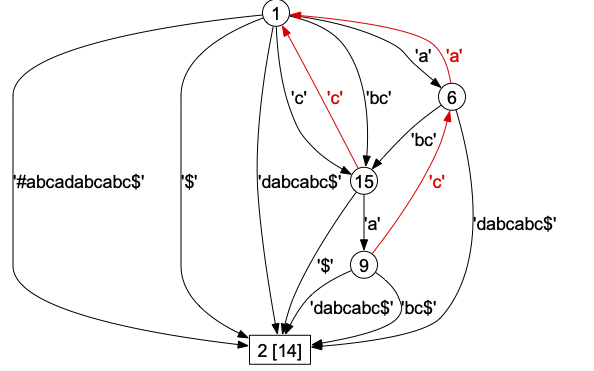
\includegraphics[height=0.4\textwidth]{fig/exp1/cdawg.png}
  %% 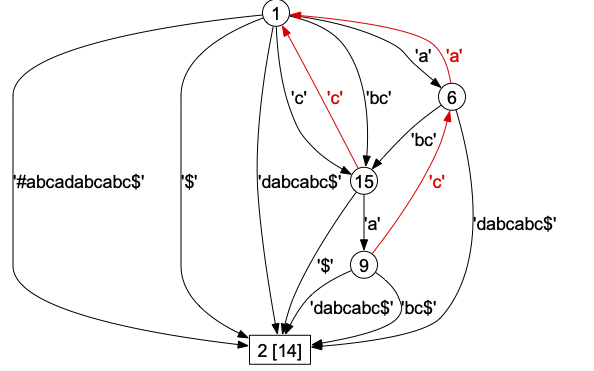
\includegraphics[height=0.4\textwidth]{fig/exp1/cdawg.pdf}
  \medskip 
  \caption{The CDAWG for a text $T = \mathtt{\#abcadabcabc\$}$ of length $13$. Its branching nodes $1, 6, 15$, and $9$ represents all of four maximal repeats $\eps, \mathtt{a}, \mathtt{abc}$, and $\mathtt{abca}$ with frequencies $14, 4, 3$, and $2$, respectively.
  }\label{fig:cdawg}
\end{figure}
%%%%%%


\subsection{Basics of enumerating maximal repeats}
Firstly, we explain the basic strategy of maximal repeat enumeration, which are common to all existing algorithms. 
Our result is obtained by combination of the top-down traversal of the virtual affix tree and efficient test for the left-branchingity based on the suffix array of a text. 
%%% 
We briefly explain our approach in the followings. 
%%We made a through survey of the existing algorithms for MR-enumeration. 

The CDAWG $\sig G$ for a txt $T$ (see \cref{fig:cdawg}) is a central data structure for dealing with  maximal repeats. It can be obtained from the suffix tree $\sig S$ (or equivalently its Weiner tree $\sig W$) for the same $T$ by merging all isomophic subtrees. Actually, what Raffinot~\cite{raffinot2001maximal} found was that that all nodes but the sink of the resuting DAG $G$, i.e., the CDAWG, represent all maximal repeats. 

On the other hand, if we view from the side of the suffix tree, all of its nodes with branching (outgoing) forward edges represent right-branching subwords of $T$, while all nodes with branching (incoming) backward edges (suffix links) represent left-branching subwords of $T$. Since maximal repeats are those subwords which are both left- and right-branching, we seek them by traversing either $\sig S$ or $\sig W$. 

Based on the above observation, we can classify enumeration algorithms by the following g two criteria: 
\begin{enumerate}[(1)]
\item The \textit{direction} of the traversal, i.e., either \textit{top-down} from the root to leaves~(\td), or \textit{bottom-up} from leaves to the root~(\bu). 
\item The \textit{types of edges} to follows, i.e., either \textit{forward}~(\fw) or \textit{backward}~(\bw). 
\end{enumerate}

\subsection{Classification of existing algorithms}

In \cref{table:summary}, we list and classify the state-of-the-art methods for MR enumeration ~\cite{narisawa2007efficient,okanohara2009linear,beller:berger2012space:efficient:bbo,belazzougui2020linear,nishimoto:cpm2021enum}. In the table, the last column ``Trav.~Type'' indicates the classification in combinations of tokens, such as $\tdfw$, the first one from $\set{\td, \bu}$ and the second one from $\set{\fw, \bw}$. 

By careful look at \cref{table:summary}, we found the existing algorithms fall into three groups below: 
\begin{enumerate}[(I)]
\item Three graph-based algorithms with type \tdfw, which has as an underlying structure either the suffix tree $\sig S$ or the CDAWG $\sig G$. 
There are no array-based algorithms with type \tdfw. 

\item Three array-based algorithms with type \tdbw, which has as an underlying structure is the Weiner tree $\sig W$. They traverse $\sig W$ based on the top-down simulation method proposed by Abouelhoda~\cite{abouelhoda2004replacing} using the BWT array and Wavelet tree. 


\item Two array-based algorithms with type \bufw, which has as an  underlying structure the suffix tree $\sig S$. They traverse $\sig S$ based on the bottom-up simulation method proposed by Kasai et al.~\cite{kasai:lee2001lcp:linear} 
using the SA and LCP arrays. 
\end{enumerate}

From the above classification, we can obtain some useful observation about the possible design of an efficient enumeration algorithm for MRs. 

\subsection{Analysis of the existing approaches}
%\subsection{Lessons learnt}
Firstly, all existing algorithms in group (I) are graph-based ones. Thus, they directly traverse the graph top-down by following forward edges without any difficulty. 
If the underlying graph $\sig G$ is isomorphic to the CDAWG of $T$, they can run in $O(e_R)$ time as desired. We can also see that there have been no existing array-based algorithms with type $\tdfw$ so far. We will come back to this issue later. 

Next, all existing array-based algorithms fall into the cases (II) and (III). 
For the case (II), algorithms has type \tdbw. They suffer from the fact that the underly tree $\sig W$ consists only of atomic backward edges. Therefore, the algorithms must traverse atomic backward edges one by one using the LF-mapping. From this reason, they must consume $\Theta(n)$ time by following a long chain of non-branching nodes until they  encounter a maximal repeat. 

For the case (III), algorithms has type \bufw. Unlike case (II), since all forward edges in the suffix tree $\sig S$ are path-compressed, they can avoid the problem with atomic edges. However, due to the bottom-up direction, they cannot make branch-and-bound search by pruning the useless subtrees. Consequently, they must travperse all of $\Theta(n)$ edges, resulting $\Theta(n)$ total running time. 

Finally, we are curious about this fact because we could not find any immediate reason by which we should avoid using the combination {\tdfw}, namely, the \textit{top-down search of the suffix tree $\sig S$ following forward edges}.  
Next, we will examine this approach further. 

\subsection{Our approach}
From the discussion in the previous subsection, the search strategy {\tdfw} seems a novel approach for efficient enumeration of maximal repeats. Actually, we can observe the following reasons to employ {\tdfw} as the basic strategy of our enumeration algorithm:  
\begin{enumerate}
\item \textit{Efficient pruning of non-maximal nodes}. Top-down search direction seems suitable to prune useless search paths than bottom-up search direction. This pruning should be efficiently done based on the left- or right-branchingity tests on indivisual nodes or subwords. This can be done by using the combination of the SA and LCP arrays with the help of the RMQ structure. 

\item \textit{Avoiding traversal of atomic edges}. Traversal with forward edges in $\sig S$ seems preferrable than that on backward edges in $\sig W$ to avoid traversal of atomic edges symbol by symbol. Since the path compression is closely related to the longest common prefixes of suffixes containing the locus of a subword, efficient test can be supported by  the LCP array with the RMQ structure, again. 
\end{enumerate}

We explain these ideas in the next section. 

%%% EOF

%% %%%% algo.tex

%%% algo.text


%%%%%%%%%%%%%%%%
\section{The Proposed Algorithm}
\label{sec:algo}

In this section, we present the first algorithm that enumerates all maximal repeats in a text $T$ of length $n$ in $O(e_R)$ time
%and $O(\sigma^2 \log e_\fn{min})$ words of working space
using precomputed arrays, namely, the suffix, inverse suffix, and LCP arrays, namely $SA[1,n], ISA[1,n]$, and $LCP[1,n]$, occupying $O(n)$ words space. It traverses the DFS over the virtual suffix tree for $T$ using the above arrays. 

In what follows, we assume any data structure for storing $SA[1,n], ISA[1,n]$, and $LCP[1,n]$, where $LCP$ is equipped with $RMQ$~\cite{bender:colton2000thelcaproblem}, using $s(n)$ words of space, after $p(n)$ preprocessing of $T$, supporting 
access to the arrays in $t_\fn{acc}(n)$ time in the worst-case. 

In Algorithm~\ref{algo:maxrep:tdfw}, we show the $O(e_R)$-time algorithm for enumerating the rich representations of all maximal repeats in a string $T$ of length $n$, when invoked with $L_0=1, R_0=n, \ell_0= RMQ_{LCP}(L_0+1, R_0)$.
It uses the SA[1..n], ISA[1..n], and RMQ structure on $LCP[1..n]$ of a text $T[1..n] \in \Sigma^n$ as underlying data structures. 

%%%%%%%%%%%%%%%%%
\begin{algorithm}[h]
  \caption{Enumerating all distinct maximal repeats in a string}\label{algo:maxrep:tdfw}
  \textbf{Procedure} \textsc{MaxRepTD}$(\tau = (L_0, R_0, \ell_0))$:\\
  %%\KwGiven{}
  \KwIn{The triple $\tau_0 = (L_0, R_0, \ell_0)$ for a right-branching substring $X$ of a text.}
  %% \KwOut{}
  \Begin{
      \textbf{output} $\tau$
      \Comment*{A maximal repeat is found}
      $C \gets \emptyset$\; 
      $\proc{BranchRepeats}(\tau_0, C)$\; 
        \For (\CM{$R - L \ge 1$ must hold}) {$(L, R)\in C$}{
          $\tau \gets (L, R, \ell)$ with $\ell \gets RMQ_{LCP}(L+1, R)$
          \Comment*{$\tau$ is right-branching}
          Decide if $\tau$ is left-branching by SA and ISA (\cref{lemold:leftmaximal:character})\; 
          \If {$\tau$ is left-branching}{          
            \textsc{MaxRepTD}$(\tau)$\; 
          }
        }
  }
\end{algorithm}
%%%%%%%%%%%%%%%%%

% %%%%%%%%%%%%%%%%%
% \begin{algorithm}[t]
%   \caption{The algorithm for enumerating the rich representations of all maximal repeats in an input text $T[1,n]$ of length $n$ in $O(e_R)$ time by traversing the virtual suffix tree for $T$ using the suffix, inverse suffix, and longest common prefix arrays, $SA, ISA$, and $LCP$ of~$T$. In the top-level, the procedure is invoked with the rich representation $(1, n, 0)$ with the empty string $\eps$. 
%   }\label{algo:maxrep:tdfw}
%   \textbf{Procedure} \textsc{MaxRepTD}$(L, R, \ell)$:\\
%   \KwIn{A rich-representation $(L, R, \ell)$ consisting of an SA-interval $[L, R]$ and an $\ell\ge 0$ for a right-branching substring $U$ of $T$}
%   %% \KwOut{}
%   \Begin{
%       \textbf{output} $(L, R, \ell)$
%       \Comment*{$(L, R, \ell) = repr(U)$}
%       $\ell_* \gets \LCE(SA[L], SA[R])$\; 
%       %%$\ell_* \gets \lcpmin(L, R)$\;       
%         \For{$(L_c, R_c, \ell_c, c)\in \proc{BranchRepeats}(L, R, \ell_*)$}{
%           %\Comment{Notes: $\exists c \in \Sigma, \forall k \in [L',R'], T[SA[k]+\ell_*] = c$}
%           $\ell' \gets \LCE(SA[L_c], SA[R_c])$
%           %%$\ell' \gets \lcpmin(L_c, R_c)$          
%           \Comment*{$(L_c, R_c, \ell_c) = repr(\rext{(Uc)})$}
%           \uIf{$|[L_c, R_c]| = 1$}{
%             continue; \Comment{Skip $(L_c, R_c, \ell_c, c)$}
%           }
%           \uElseIf (\Commentblock{\cref{lemold:leftmaximal:character}}) {$(L_c, R_c, \ell_c)$ is left-branching }{          
%             \textsc{MaxRepTD}$(L_c, R_c, \ell_c)$\; 
%           }
%           \Else{
%             \Comment{Pruning descendants of non-left maximal substrings}
%           }
%         }
%   }
% \end{algorithm}
% %%%%%%%%%%%%%%%%%

%% \subsection{Outline of the Algorithm}
%% %%%%%
  %% The key idea of our algorithm is to combine the virtual \textit{top-down traversal} of the suffix tree of $T$ with the suffix and LCP arrays of $T$, proposed by Abouelhoda, Kurtz, and Ohlebusch~\cite{abouelhoda2004replacing}, and the $O(1)$-time left-branching test by Narisawa \textit{et al.}~\cite{narisawa2007efficient}.

For any text $T$, the suffix tree of $T$, denoted by $\stree(T)$, is an edge-labeled tree $C = (V, E, F)$. 
By \cref{def:stree}, we observe the following facts: 
\begin{itemize}
\item The node set $V$ of the suffix tree corresponds to the set of right-branching substrings in $T$. 
  
\item The nodes of $V$ are classified into two subsets: (i) all branching nodes, $W$, correspond to all right-branching repeats in $T$ such that $\occ(W)\ge 2$, and (ii) all leaves, $W$, correspond to all suffixes of $T$ such that $\occ(W) = 1$. 
  
\end{itemize}


Thus, a natural strategy to enumerate $\M(T)$ is visiting all branching nodes $W$ of $V$, which correspond right-branching repeats in $\RM(T)$, by the depth-first search of $\stree(T)$. (See appendix)

\begin{toappendix}    
Thus, a natural strategy to enumerate $\M(T)$ is visiting all branching nodes $W$ of $V$, which correspond right-branching repeats in $\RM(T)$, by the depth-first search of $\stree(T)$ are described as follows:
\begin{enumerate}[(1)]
\item Initially, we start with $\rext{\eps} = \eps$ as the root. Surely, it belongs to $\RM(T)$ because we assumed that $|\Sigma|\ge 2$. 
\item At each iteration with a visited node $U\in \RM(T)$, we enumerate chiledren $W$ of $U$ as follows: for each character $b \in \Sigma$ such that $\occ(Ub) \ge 1$, we compute the right-branching extension $W = \rext{Ub}$ of $U$ as a child. 

\item Then, we perform the following process with each child $W$:
  \begin{enumerate}[(a)]
\item When it reaches a non-repeat $W$ such that $\occ(W) = 1$, we backtrack.
\item Otherwise, it reaches a repeat $W$. In this case, $W \in \RM(T)$ is ensured.
  Then, we check if it is left-branching, namely, if $W \in \LM(T)$ holds.
  (3.b.i) If so, $W$ belongs to $\M(T) = \LM(T)\cap \RM(T)$, and thus, output it as an answer.
  (3.b.ii) Otherwise, at this moment, we are not sure if we should continue the search of the descendants of $W$, or we should stop the search. Below, we discuss this case. 
  \end{enumerate}
\end{enumerate}
\end{toappendix}


%%%%%%
\begin{figure}[t]
\centering  
  \includegraphics[width=0.85\textwidth]{fig/exp1/fwdstree.pdf}
  \caption{The suffix tree for a text $T = \mathtt{\#abcadabcabc\$}$.}\label{fig:fwdstree}
\end{figure}
%%%%%%

Now, the remaining problems are summarized as follows:
\begin{enumerate}[(i)]
\item How to prune non-maximal descendants. 

\item How to make top-down traversal following forward edges in $O(1)$ time per edge. 

\item How to efficiently test the left-branching in $O(1)$ time per node. 
\end{enumerate}

In what follows, we will show how to efficiently solve these problems using arrays $SA, ISA$, and $LCP$ with auxliary data structures. 

\subsection{How to prune non-maximal descendants}
%%% \subsection{Subproblem A.1: how to prune non-maximal descendants of a node}
%%%%%

Recall that all nodes of the suffix tree of a text $T$ correspoind to right-branching substrings of $T$, namely, the elements of $\RM(T)$. 
For the choice in the case (3.b.ii) above, we have the next lemma. 

\begin{lemma}[Weiner link property]
\label{lemold:weiner:property}
Let $U$ and $W$ be any substrings of $T$ associated with nodes of the suffix tree. If $U$ is a prefix of $W$, then $W \in \LM(T)$ implies $U \in \LM(T)$. 
\end{lemma}

\begin{proof}
Suppose that $W \in \LM(T)$. It folows that there exist some distinct positions $p, q \in \spos(W)$ with $p\not= q$ such that the characters at the preceding positions are mutually distinct, i.e., $T[p-1]\not = T[q-1]$. By assumption, $U$ is a prefix of $W$. Combining this assumption and \cref{lemold:occ:monotonicity}, it follows  that $p,q \in \spos(W) \subseteq \spos(U)$. Hence, the claim is proved. 
\qed
\end{proof}

From \cref{lemold:weiner:property} above, we know that we can safely prune the search of descendants when the case of (3.b.ii)  happens.
For example, in \cref{fig:fwdstree}, we observe that every left-branching node (indicated by red circles) has at least two outgoing Weiner links (indicated by red lines). Then, we can examine that the Weiner link property in \cref{lemold:weiner:property} holds for all ancestors of any left-branching nodes. 
%% that is, if a node has at least two red outgoing edges. so are all ancestors of it. 

\subsection{How to make top-down traversal following forward edges}
%%\subsection{Subproblem A.2: how to compute the children by right-branching extension}
%%%%%


% %From \cref{lemold:lcpmin:rm}, 
% To obtain a child of a given $\tau = (L, R, \ell)$ for a substring $W$, we compute the SA-interval $[L_c, R_c]$ for the substring $Wc$ obtained from $W$ by appending a character $a \in \Sigma$ to $W$, and finds its length by computing $\ell = \LCE(SA[L], SA[R])$. Then, we can show that the substring represeted by the triple $(L_c, R_c, \ell)$ is right-branching in $T$. 

From now on, we explain how to list child intervals from the parent interval in the followings. 
We inductively suppose that a parent maximal repeat $U$. This means that the rich representation $(L,R,\ell)$ of $U$ satisfies the conditions: (i) $|[L,R]| = R - L + 1 \ge 2$ and (ii) $\LCE(SA[L], SA[R]) = \ell$, where the value $\LCE(SA[L], SA[R])$ can be computed by the range-minima of $LCP$ on the range $[L+1,R]$.
We let $\op{Follow}(L, R, \ell) := \set{SA[k]+\ell \mid k \in [L, R]} \subseteq \Sigma$ to be 
the set of distinct characters that occur in $T$ at positions following the end positions of $W$.

\begin{definition}[forward range distinct query~\cite{abouelhoda2004replacing}]
Given the rich representation $(L,R,\ell) = \repr(U)$ for a maximal repeat $U = \rext U$, we define the \textit{forward range distinct query} with $(L,R,\ell)$, denoted by $\op{BranchRepeats}(L, R, \ell)$, as the query to return the list $\op{BranchRepeats}(L, R, \ell)$ of all triples $(L_c, R_c, c)$ such that
\begin{enumerate*}[(i)]
\item $c \in \op{Follow}(L, R, \ell)$, 
\item $[L_c, R_c] = \intr(Uc)$, and 
%%\item $\ell = \op{lcpmin}(L_c, R_c)$. 
\end{enumerate*}
\end{definition}

%%%Based on \cref{lemold:child:interval:chara},
In Algorithm~\ref{algo:BranchRepeats}, we present the recursive procedure that lists $k\ge 0$ child ranges $(L_1, R_1, \ell_1), \dots, (L_k, R_k, \ell_k)$ of a given range with width at least two when invoked with an input range $[L, R]$, $\ell_* = RMQ_{LCP}(L+1, R)$, and $C = \emptyset$.

%%%%%%%%%%%%%%%%%
\begin{algorithm}[h]
  \caption{
    The recursive procedure for listing $k\ge 0$ child ranges with width at least two given the triple for a right-branching substring. 
  }\label{algo:BranchRepeats}
  \textbf{Procedure} \proc{BranchRepeats}$(L, R, \ell_*, C)$:\\  
  \KwGiven{RMQ structure on the LCP array of a text}
   \KwIn{Integers $1\le L\le R\le n$, $\ell_*\ge 0$, and the pointer $C$ to a set of triples}
  %% \KwOut{}
  \Begin{
      \If {$R - L \ge 1$}
      {
        $(M, \ell) \gets RMQ_{LCP}(L+1, R)$
        \Comment*{$\ell = LCP[M]$}
        \iIf {$\ell_* < \ell$}{
          $C \gets C \cup \set{(L, R, \ell)}$
          \Comment*{$[L,R]$ is monotone}
        }
        \Else  (\CM{$\ell_* = \ell$} and $[L,R]$ is diverse) 
        {
          $\proc{BranchRepeats}(L, M-1, \ell_*, C)$\; 
          $\proc{BranchRepeats}(M, R, \ell_*, C)$\;
        }
      }
      \Return $C$\; 
  }
\end{algorithm}
%%%%%%%%%%%%%%%%%

  \begin{lemma}
For a right-branching substring $U$ and a $c\in \Sigma$, if a triple $\tau = (L_c, R_c, c)$ satisfies the conditions (i)--(ii) and $\occ(Uc)\ge 1$ and if $\ell_c := \lcpmin(L_c, R_c)$, then $(L_c, R_c, \ell_c)$ is the rich representation for the maximal repeat $W = \rext{(Uc)}$. 
\end{lemma}

% To list appropriate child SA-intervals from a the parent interval, we use a data structure for forward range distinct query, denoted by $\op{BranchRepeats}(L, R, \ell)$, proposed by Abouelhoda \textit{et al.}~\cite{abouelhoda2004replacing} as follows.




% %%%%%%%%%%%%%%%%%
% \begin{algorithm}[t]
%   \caption{The algorithm for answering the forward range distinct queries for a text $T$ with  the suffix, inverse suffix, and LCP arrays and the LCE structure. It runs in $O(1)$ time per child range to output. 
%   }\label{algo:BranchRepeats}
%   \textbf{Procedure} \proc{BranchRepeats}$(L, R, \ell_*; LCP)$:\\  
%    \KwIn{A rich representation $(L, R, \ell_*)$ with SA-interval $[L, R]$ and length $\ell_*$ such that $\ell_* = \LCE(SA[L], SA[R])$}
%   %% \KwOut{}
%   \Begin{
%       \uIf (\CM{Case~1: $|[L,R]| = 1$}) {$R - L + 1 = 1$}{
%         \Return $([L, R], c)$ with $c \gets T[SA[L]+\ell_*]$\; 
%       }
%       \Else (\CM{Case~2: $|[L,R]| \ge 2$}) {
%         $M \gets \LCE(SA[L], SA[R])$\; 
%         %\Comment*{Notes: $LCP[M] = \min LCP[L, R]$}
%         \uIf (\CM{Case~2.a: $[L,R]$ is monotone}) {$LCP[M] > \ell_*$}{
%           \Return $([L, R], c)$ with $c \gets T[SA[L]+\ell_*]$\;
%         }
%         \uElseIf  (\CM{Case~2.b: $[L,R]$ is diverse}) {$LCP[M] = \ell_*$}{
%           $D_0 \gets \proc{BranchRepeats}(L, M-1, \ell_*; LCP)$\; 
%           $D_1 \gets \proc{BranchRepeats}(M, R, \ell_*; LCP)$\;
%           \Return the list $D$ obtained by concatenating $D_0$ and $D_1$\; 
%         }
%         \Else ({$\rhd$ $LCP[M] < \ell_*$}) {
%           \Comment{This case never occur}
%         }
%       }
%   }
% \end{algorithm}
% %%%%%%%%%%%%%%%%%

  To compute $\op{Follow}(L, R, \ell)$, we use the LCP array to shift the positions in $\set{SA[k] \mid k \in [L, R]}$ by the displacement $\ell = |U|$  with the LCP array using the technique following~\cite{abouelhoda2004replacing,ohlebusch2013bookbioinfo}.
Assume that $\repr(U) = (L, R, \ell)$ satisfies the above conditions. Clearly, it holds that $LCP[k] \ge \ell = \lcpmin(L, R)$ for any rank $L+1 \le k\le R$. The lemma below describes when the equality holds. 

\begin{lemmarep}[Abouelhoda \textit{et al.}~\cite{abouelhoda2004replacing}]
\label{lemold:child:interval:chara}
Assume that $\repr(W) = (L, R, \ell)$ satisfies the above conditions.
For any subinterval $[L', R']$ of $[L,R]$, 
the condition $|\op{Follow}(L', R', \ell)| \ge 2$ holds if and only if 
there exists a rank $k \in [L+1, R]$ such that $LCP[k] = \ell$. 
\end{lemmarep}

\begin{proof}
Suppose that $LCP[k] > \ell$ for all $k \in (L, R]$.
If we let $\ell_* := \min\sete{ LCP[k] \mid k \in (L',R'] }$, the set of suffixes have the common prefix $P$ of length $\ell_*$. Since $\ell_* > \ell$, they have a common character $c := P[\ell] \in \Sigma$ at the position following $\epos(U)$, and thus, the if-direction is proved. The only-if direction is also shown by similar discussion. For detalis, please see \cite[Lemma~4.3.5]{ohlebusch2013bookbioinfo}.
\qed
\end{proof}

Based on \cref{lemold:child:interval:chara}, we show the correctness of Algorithm~\ref{algo:BranchRepeats}. 
%% we show Algorithm~\ref{algo:BranchRepeats} for implementing the forward range distinct query $\op{BranchRepeats}(L, R, \ell)$. 



\begin{lemma}[Abouelhoda \textit{et al.}~\cite{abouelhoda2004replacing,ohlebusch2013bookbioinfo}]
\label{lemold:algofst:BranchRepeats}
Algorithm~\ref{algo:BranchRepeats} correctly implements the forward range distinct query $\op{BranchRepeats}(L, R, \ell)$ in $O(h\cdot t_\fn{acc})$ time, where $t_\fn{acc}$ denotes the operation time for accessing to $SA, ISA$, and a text $T$ of length $n$. 
\end{lemma}

The above lemma says that we can enumerate all children of a given parent node in the suffix tree for $T$ in $O(1)$ amortised time per child in rich representations.    

% %%%%%%%%%%%%%%%%%
% \begin{algorithm}[t]
%   \caption{The algorithm for deciding if a given SA-interval $[L,R]$ is left-branching with respect to an input text $T[1,n]$ in $O(1)$ time with the suffix and the inverse suffix arrays, where $1\le L\le R \le n$.
%   }\label{algo:MaxRepeats}
%   \textbf{Procedure} \textsc{IsLeftMaximal}$(L, R; SA, ISA, T)$:\\  
%    %% \KwIn{}
%   %% \KwOut{}
%   \Begin{
%       $(p, q) \gets (SA[L], SA[R])$\;
%       \iIf{$(p=1)\lor (q=1)$}{
%         \Return $\op{True}$\; 
%       }
%       \iElseIf{$T[p-1]\not= T[q-1]$}{
%         \Return $\op{True}$\; 
%       }
%       \iElseIf{$(R - L) = (ISA[p-1] - ISA[q-1])$}{
%         \Return $\op{True}$\; 
%       }
%       \iElse{
%         \Return $\op{False}$\; 
%       }
%   }
% \end{algorithm}
% %%%%%%%%%%%%%%%%%

%%%% \subsection{Subproblem A.3: how to check if a child is left-branching}

\subsection{How to test if a given triple is left-branching in constant time}
%% \subsection{Testing the left-branching of substrings with the suffix, inverse suffix, and lcp arrays}
%%%%%

The second task is to decide the left-branching of a child in the rich representation. 
% Related to this problem, Narisawa, Inenaga, Bannai, and Takeda~\cite{narisawa2007efficient} presented an efficient procedure to decide the left-branching of a substring $T[p,q]$ represented by a pair $p, q$ of positions using $SA, ISA$, and $LCP$.

\begin{itemize}\item[] 
\textsc{Left-Branching Test}:  
Given the triple $\tau$ for a substring $W$, 
if $R - L \not= ISA[SA[L]-1] - ISA[SA[R]-1]$ holds, then $W$ is left-branching, and otherwise, it is not. 
\end{itemize}


The following lemma is an extension of the characterization of the left-branching by Narisawa \textit{et al.}~\cite[Lemma~10]{narisawa2007efficient}. 

\begin{lemma}[left-branching test]\label{lemold:leftmaximal:character}
Let $(L,R, \ell)$ be the rich representation of any substring $W$ of $T$. 
%We let $(p, q) = (SA[L], SA[R])$. 
Then, the following conditions (1)--(3) are equivalent each other: 
\begin{enumerate}[(1)]
\item $W$ is not left-branching in $T$. 
\item $BWT[L, R]$ is monotone. 
\item $(R - L + 1) = (ISA[SA[L]-1] - ISA[SA[R]-1] + 1)$. 
\end{enumerate}
\end{lemma}

\begin{proof} 
We let $p = SA[L], q = SA[R]$. 
$(1)\Implies (2)$: Suppose that $W$ is not left-branching in $T$. Then, we see that all occurrences of $W$ in $T$ have the same character, say $c$, in the previous positions in $\spos(W)$. Thus, the claim (2) immediately follows. 
%%% 
$(2) \Implies (3)$: We can easily observe that the function $f(k) := ISA[SA[k]]$ realizes the LF-mapping~\cite{Ferragina05:FM} by definition. Hence, claim (3) immediately follows from (2). 
%%% 
$(3) \Implies (1)$: 
%We show the contraposition $\neg (1) \Implies \neg (3)$. 
Suppose that $W$ is left-branching in $T$. Then, it follows that $c = T[p-1]\not= T[q-1] = d$ for some $p, q \in\spos(W)$ of $W$. 
%It follows that the subarray $BWT[L,R]$ contains mutually distinct $c$ and $d$. Since $[L,R]$ is the SA-interval of $W$, 
Therefore, the substring $W$ has a pair of distinct characters $c = T[p-1]$ and $d = T[q-1]$ at the previous positions of its start positions. By contraposition, $W$ is left-branching. 
Combining the above arguments, the lemma is proved. 
\qed   
\end{proof}


From \cref{lemold:leftmaximal:character}, the next lemma immediately follows. 

%can check the left-branching using $SA$ and $ISA$. 
%such that $W$ is left-branching in $T$ if and only if $(R - L + 1) \not= (ISA[p-1] - ISA[q-1] + 1)$. 
% Therefore, we have the next lemma. 

\begin{lemma}
\label{lemold:algofst:leftmaximal:algo}  
Given  the rich representation~$\tau = (L, R, \ell)$ of a substring, we can decide if
  $\tau$ represents a left-branching substring in $O(t_\fn{acc}(n))$ time and $O(1)$ working space, where $t_\fn{acc}(n)$ denotes the access time to arrays $SA, ISA$ and $T$. 
\end{lemma}



\subsection{Correctness and time complexity}
%%%%%
Combining \cref{lemold:weiner:property}, \cref{lemold:algofst:BranchRepeats}, and \cref{lemold:algofst:leftmaximal:algo} shown in this section, we prove \cref{thmold:algo:maxrep:main}, the main result of this paper.  
  

% \begin{theorem}[correctness and complexities of Algorithm~\ref{algo:maxrep:tdfw}]\label{thmold:algo:maxrep:main}
%   The set $\M(T)$ of all maximal repeats in a text $T$ of length $n$ can be enumerated 
%   in $O(e_R\cdot t_\fn{acc}(n))$ time and $O(\sigma^2 \log e_R)$ words of working space
%   using the suffix, inverse suffix, and LCP arrays for $T$ 
%   occupying $O(s(n))$ words of space after $O(p(n))$ preprocessing, where $t_\fn{acc}$, $p(n)$, and $s(n)$ denote the access time, preprocessing, and space of the data structure implementing arrays $SA, ISA$, and $LCP$ with $RMQ$ of a text $T$. 
% \end{theorem}

\begin{proof}
  The correctness and time complexities follows from \cref{lemold:weiner:property}, \cref{lemold:algofst:BranchRepeats}, and \cref{lemold:algofst:leftmaximal:algo}. To bound the working space by $O(\sigma^2 \log e_R)$, we apply the heavy-leaf decomposition to computation tree of the DFS by  \textsc{RecMaxRepeatsFwd} following Belazzougui and Cunial~\cite[Lemma~4.2]{belazzougui2020linear} (see also \cite{hoare1962computj:quicksort}). 
  At each iteration, we select the child with the widest range first, which has the largest number of leaves.
  (Although $\CDAWG(T)$ has fewer  nodes than $\stree(T)$ by merging isomorphic subtrees, this does not matter in our analysis.) Consequently, this modified DFS yields at most $O(\log n)$ levels with $O(\sigma)$ side information per level, each has $O(1)$ size (i.e., bidirectional rich representations) in the DFS. This leads to the working space is $O(\min\set{e_R, \sigma\log n}) = O(\sigma\log n)$ words. This completes the proof. \qed 
\end{proof}


From \cref{thmold:algo:maxrep:main}, we can immediately show \cref{thmold:algo:maxrep:classic} and \cref{thmold:algo:maxrep:derived} 
by substituting different SA implementations for the $SA$- and $LCP$-oracles~\cite{gagie:navarro:prezza2020fully,kempa:kociumaka2023collapsing}. 
%%% 
By simulating a \textit{bidirectional index} for $T$ and its reversal $T\rev$ with of a pair of the SA- and LCP-indices for them, we can obtain enumeration of $\M(T)$ in $O(\min\set{e_L, e_R})$ time close to one by Raffinot~\cite{raffinot2001maximal}. 
Let $e_\fn{min} = \min\set{e_L, e_R}$ is the minimum of the sizes of $\CDAWG(T)$ and $\CDAWG(T\rev)$. 
We remark that it is shown by Inenaga and Kosolobov~\cite{inenaga:kosolobov2024relating:left:right} that $e_R$ is at most $\sqrt{n}$ times larger than $e_L$, and vice versa. 
% On the relationship between $e_R$ and $e_L$, we remark that it is recently shown by Inenaga and Kosolobov~\cite{inenaga:kosolobov2024relating:left:right} that the ratio $\frac{e_L}{e_R}=\Theta(\sqrt n)$ hold for all texts. 

% \begin{theorem} \label{thmold:algo:maxrep:bidirect}
% An $O(\min\set{e_L, e_R})$-time and $O(n)$-space algorithm based on a two copies of the classical suffix and LCP arrays (Manber and Myers~\cite{manber:myers1993suffixarrays}) with the RMQ structure (e.g.~\cite{bender:colton2000thelcaproblem}), one for $T$ and the other for $T\rev$. 
% % 
% The set $\M(T)$ can be enumerated in $O(e_\fn{min})$ time and $O(\sigma^2\log e_\fn{min})$ words of working space using the bidirectional index consisting of 
% $SA, ISA$, and $LCP$ for a text $T$ and $SA\rev, ISA\rev$, and $LCP\rev$ for $T\rev$ with total space $O(n)$ words, where $e_\fn{min} = \min\set{e_L, e_R}$ is the minimum of the sizes of $\CDAWG(T)$ and $\CDAWG(T\rev)$. 
%% \end{theorem}

% \begin{proof}
% From \cref{cor:fst:enum:arrays} and the proof of \cref{thmold:raffinot:mr:cdawg}, the claim follows. \qed. 
% \end{proof}





%%%%%%
\begin{figure}[t]
\centering  
  \includegraphics[width=0.75\textwidth]{fig/turu/figturu2.pdf}
  \caption{An example run of Algorithm~\ref{algo:maxrep:tdfw} for a text $T = \mathtt{\#aabaababb\$}$.
    %% Circles and solid black arrows, indicate the nodes and forward of the suffix tree of $T$.
    %% Gray and white nodes are left-branching and non-left-braning nodes. To each node, its string label $W$ and the rich representation $([L, R], \ell)$ of $W$ are attached. Solid red arrows designate the search path of the algorithm which follows reverse edges as long as they are left-branching.
}\label{fig:run:example}
\end{figure}
%%%%%%

\subsection{Execution example}

In \cref{fig:run:example}, we show an example run of Algorithm~\ref{algo:maxrep:tdfw} for a text $T = \mathtt{\#aabaababb\$}$. Circles and solid black arrows, indicate the nodes and forward of the suffix tree of $T$.
    Gray and white nodes are left-branching and non-left-braning nodes. To each node, its string label $W$ and the rich representation $([L, R], \ell)$ of $W$ are attached. Solid red arrows designate the search path of the algorithm which follows reverse edges as long as they are left-branching.



% \subsection{Applications}
% We remark that \cref{thmold:algo:maxrep:main} provides a general time and space bound parameterized with the implementation of $SA, ISA$, and $LCP$. Hence, we obtain different time and space bounds from \cref{thmold:algo:maxrep:main} by substituting a particular implementation of these arrays into Algorithm~\ref{algo:maxrep:tdfw}. 

% First, we consider the case of the standard array representation of $SA, ISA$ ,and $LCP$ with $t_\fn{acc} = O(1)$ and $s = n$ (Manber and Myers~\cite{ManberM93:SA}). In this case, we have the next result. 

% \begin{corollary}[standard array indexes]\label{cor:fst:enum:arrays}
% The set $\M(T)$ of all maximal repeats in an input text of length $n$ can be enumerated in $O(e_R)$ time and $O(\sigma^2\log e_R)$ words of working space with the arrays $SA, ISA$, and $LCP$ for $T$ using total space $O(n)$, after $O(n)$ time of preprocessing on $T$. 
% \end{corollary}

% This is the first array-based algorithm that enumerates all maximal repeats with the running time same the algoritm by Raffinot~\cite{raffinot2001maximal} based on the CDAWG, whose running time is linear in the size of the CDAWG for the same text. 

% Next, we consider the case for compressed indexes for highly repetitive data~\cite{navarro2021indexing:ii}. 
% Gagie, Navarro, Prezza~\cite{GagieNP20:RLBWT} proposed a compressed text indexing data structure based on the run-length BWT for a text $T$, called the \textit{r-index}. In this case, we have the following result. 

% \begin{corollary}[compressed index for repetitive texts]\label{cor:fst:enum:arrays}
% The set $\M(T)$ of all maximal repeats in an input text of length $n$ can be enumerated in $O(e_R \log(n/r))$ time and $O(\sigma^2\log e_R)$ words of working space with the r-index\cite{GagieNP20:RLBWT} for $T$ using total space $O(r\log n)$, after $O(n(\log r + \log\log_w(n/r)))$ preprocessing of $T$. 
% \end{corollary}

% \begin{proof}
% When $BWT$ has $r$ runs with $r \le n$, for any constant $s > 0$, the data structure support access operation to $SA, ISA$ ,and $LCP$ in  $t_\fn{acc} = O(\log(n/r))$ time using $s = O(rs)$ words of space and $O(n(\log r + \log\log_w(n/r)))$ construction time (Gagie \textit{et al.}~\cite[Appendix]{GagieNP20:RLBWT}), where $w = \floor{\log n}$ is the machine word size.  By selecting $s = \log n$, we have the claimed complexities. 
% \qed 
% \end{proof}

% Considering enumeration of $\M(T)$ in $O(\min\set{e_L, e_R})$ time close to one by Raffinot~\cite{raffinot2001maximal} (\cref{thmold:raffinot:mr:enum}), it is natural to use a \textit{bidirectional index}, which is merely a pair of the copies of standard indexing arrays $SA, ISA$, and $LCP$ for $T$ and $T\rev$. Then, we have the following results. 

% \begin{theorem} \label{thmold:algo:maxrep:bidirect}
% The set $\M(T)$ can be enumerated in $O(e_\fn{min})$ time and $O(\sigma^2\log e_\fn{min})$ words of working space using the bidirectional index consisting of 
% $SA, ISA$, and $LCP$ for a text $T$ and $SA\rev, ISA\rev$, and $LCP\rev$ for $T\rev$ with total space $O(n)$ words, where $e_\fn{min} = \min\set{e_L, e_R}$ is the minimum of the sizes of $\CDAWG(T)$ and $\CDAWG(T\rev)$. 
% \end{theorem}

% \begin{proof}
% From \cref{cor:fst:enum:arrays} and the proof of \cref{thmold:raffinot:mr:cdawg}, the claim follows. \qed. 
% \end{proof}

% On the relationship between $e_R$ and $e_L$, we remark that it is recently shown by Inenaga and Kosolobov~\cite{inenaga:kosolobov2024relating:left:right} that the ratio $\frac{e_L}{e_R}=\Theta(\sqrt n)$ hold for all texts. 


  


%%using precomputed array-like index structures occupying $O(n)$ words space. 


%% %%% debug 
%% %%%%%%%%%%%%%%%%%
%% \def\Procedure{\Statex\hspace-1.0\leftmargin\textbf{Procedure}}
%% \begin{algorithm}[t]
%%   \caption{The algorithm $\textsc{ExtendBoth}(L,R,\ell)$ that, given the rich representation $(L,R, \ell)$ of a substring $W$ such that $R - L + 1 \ge 1$, returns the rich representation $(L_*,R_*,\ell_*)$ of the unique maximal repeat $\mext{W}$ containing $W$ using the forward arrays $(SA, ISA, LCP)$ for $T$ and the reverse arrays $(SA\rev, ISA\rev, LCP\rev)$ for $T\rev$. 
%%   }\label{algo:ExtendBoth}
%%   %% \begin{algorithmic}[1]
%%   \textbf{Procedure} \textsc{ExtendBoth}$(L, R, \ell; \sig I, \sig I\rev)$
%%   \Comment*{input: $repr(W) = (L, R, \ell)$}
%%   $\ell' \gets \lcpmin(L+1, R)$ \Comment*{maximally extending rightwards}
%%   $(L\rev,R\rev) \gets \textsc{ReverseInt}((L, R, \ell'), SA, ISA\rev, LCP\rev)$
%%   \Comment*{reverse side}  
%%   $\ell_* \gets RMQ_{LCP\rev}(L+1, R)$ \Comment*{maximally extending leftwards}
%%   $(L_*,R_*) \gets \textsc{ReverseInt}((L\rev, R\rev, \ell_*); SA\rev, ISA, LCP)$
%%   \Comment*{forward side}
%%   \textbf{return} $(L_*,R_*,\ell_*)$ 
%%   \Comment*{output: $repr(\mext{W}) = (L_*, R_*, \ell_*)$}
%% \end{algorithm}
%% %%%%%%%%%%%%%%%%%%%

%% %%%%%%%%%%%%%%%%%
%% \begin{algorithm}[t]
%%   \caption{
%%     The algorithm \textsc{ReverseInt} for converting
%%     a given forward SA-interval $[L_+, R_+]$ of a substring $W$ in $SA_+$
%%     into the reverse SA-interval $[L_-, R_-]$ of $W\rev$ in $SA_-$. 
%%     using the $SA_+$, $ISA_{-}$, and $LCP_{-}$. 
%%   }\label{algo:ExtendBoth}
%%   \textbf{Procedure} \textsc{ReverseInt}$((L_+, R_+), SA_+, ISA_-, LCP_-)$:\\
%%     %% \KwIn{The forward triple representation $(L_+, R_+, \ell)$ of $W$ and the suffix array $SA_+$ in one direction, and the inverse suffix array $ISA_-$ and the longest common prefix array $LCP_-$ in the opposite direction.}
%%   %% \KwOut{The triple representation $\op{repr}_-(W_-) = (L_-, R_-, \ell)$ of the reversed substring $W_-$ in the reverse suffix array $SA\rev$.}
%%   \Begin{
%%     %% $k_+ \gets \text{arbitrary rank in } [L, R]$\; 
%%     %% $p_+ \gets \SA_+[k_+]$ 
%%     %%   \Comment*{the start position of $\rext{W}$ in $T_+$}
%%     %% $p_- \gets n - p_+ - \ell +\,1$
%%     %%   \Comment*{the end position of $\rext{W}$ in $T_-$}
%%     %% $k_- \gets \ISA_-[p_-]$ 
%%     %% \medskip  
%%     %% $k_+ \gets \text{arbitrary rank in } [L, R]$\; 
%%     Select arbitrary rank $k_+$ in $[L, R]$\; 
%%     Compute the reversed rank $k_- \gets \ISA_{-}[ q ]$ of the end position $q := n - (\SA_+[k_+]) - \ell +\,1$ of $W\rev$\;  
%%     $L_- \gets \min\set{ L_- \mid (L_- \le k_-) \land (\ell \le LCP_-[L_-]) }$\;
%%     $R_- \gets \max\set{ R_- \mid (k_- \le R_-) \land (\ell \le LCP_-[R_-]) }$\;
%%     \textbf{return} $[L_-, R_-]$ 
%%   }
%%     %% \Comment*{$\op{repr}(\rext{W}) = (L_-, R_-)$}
%% \end{algorithm}
%% %%%%%%%%%%%%%%%%%

  %% In Algorithm~\ref{algo:outline:forward:maxrep}, we show an abstract scheme of our first algorithm in terms of substring representation of maximal repeats, using the maximal right-extension operaton $\rext{\cdot}$ over substrings. Later, we will see the implementation of this scheme in SA-interval representation of substrings. 

%% In the following, we will proceed with first showing that the call 
%% $\textsc{RecMaxRepeats}(\rext{\eps})$
%% of the scheme correctly enumerates all maximal repeats contained an input text $T[1,n]$ in $O(e_R)$ time, and then, with giving  efficient implementation of all parts of the scheme using the suffix, inverse suffix, and lcp arrays. 
  

%% Let us consider the suffix tree $Stree(T)$ for $T$. It is well-known that the vertice set of $Stree(T)$ coincides the set $\sig R$ of all right-branching substrings in $T$. Thus, we can apply \cref{lemold:weiner:property} to all branching nodes of the suffix tree. Precisely, the subset $\sig M$ of $\sig R$ consisting of all left-branching nodes are closed under taking prefixes. In other words, the set $\sig M$ of all maximal repeats is monotone w.r.t.~the prefix order over right-maximal substrings in $T$. 

%% From the above observation, we adopt that the following \textit{search strategy} over all nodes of the suffix tree, which is sound for the set $\sig M$ of all maximal repeats. 
%% \begin{itemize}
%% \item (a) Initially, we start from the root node of $STree(T)$. 
%% \item (b) At any iteration with a node $u$ with the string label $U = str(u)$, we test if $U$ is left-branching. (b.1) If so, we print $U$ as a maximal repeats, and then continue the search for all children $w$ of $u$; (b.2) Otherwise, we prune the subtree below $u$, and backtrack to the parent of $u$. 
%% \end{itemize}

%% \cref{lemold:weiner:property} ensures that the above strategy does not miss any maximal repeats since the parent of a maximal repeat in $STree(T)$ is also a maximal repeat. 

  %% %%%%%%%%%%%%%%%%%
%% \medskip
%% \begin{algorithm}[h]
%% \caption{An algorithm scheme for maximal repeat enumeration.
%% }\label{algo:outline:forward:maxrep}
%%   % \caption{An algorithm scheme for enumerating all maximal repeats contained an input text $T[1,n]$ in $O(e_R)$ time with the suffix, inverse suffix, and longest common prefix arrays.
%%   % }\label{algo:outline:forward:maxrep}
%%   \textbf{Procedure} \textsc{RecMaxRepeats}$(W)$:\\
%%   \KwIn{a right-maximal substring $W$ of $T$ such that $\rext W = W$}
%%   %% \KwOut{}
%%   \Begin{
%%       \textbf{output} $W$\;
%%         \For{$c \in \proc{BranchRepeats}(W)$}{
%%           %% $y \gets \rext{(Wc)}$\;
%%           \uIf{$\rext{(Wc)}$ is left-branching}{
%%             \textsc{RecMaxRepeats}$(\rext{(Wc)})$\; 
%%           }
%%           \Else{
%%             \textbf{continue}; \Comment{Prune this branch with $c$}
%%           }
%%         }
%%   }
%% \end{algorithm}
%% %%%%%%%%%%%%%%%%%

  

%% The first task is the computation of the forward range distinct queries with a substring $W$, which asks if the set of unique characters The above query is not the reversed version of the standard range distinct queries. This is because the SA-interval $[L,R]$ holds the set $SPos_T(W) := \set{SA[L], SA[L+1], \dots, SA[R]}$ of the starting positions of all occurrences of $W$. However, we want to have the set $BranchRepeats(L, R)$ of distinct characters occuring at the positions following the end positions, namely, the set $EPos_T(W)+1 := \set{SA[L]+\ell+1, SA[L+1]+\ell+1, \dots, SA[R]+\ell+1}$ of the end positions of $W$. 
%% If we are given the SA-interval for this set $EPos_T(W)+1$, then the set $BranchRepeats(L, R)$ can be easily computed. However, it is not easy to compute $BranchRepeats(L, R)$ directly from the SA-interval $[L,R]$. 




%%%% EOF
%%new
%% \section{Conclusion}
\label{sec:conc}
%% \section{Summary and discussions}
In this paper, we considered the problem of enumerating maximal repeats in a text, one of the most fundamental problems in string algorithms, we presented the first output-sensitive algorithms for enumerating all maximal repeats in a text in time proportinal to the size of the corresponding CDAWG. 

Since the proposed algorithm relies only on access to a set of array data structures as a blackbox, we expect that it will benifit from the future development of these data structures without any additional cost. Moreover, it is a simple and efficient array-based algorithm. Hence, we hope that our algorithm will be able to replace the role of the CDAWGs large-scale sequence analysis applications.


%% %%=======
%% %%% intro.tex
\newpage
\section{Introduction}

\subsection{Backgrounds}

Detection of all patterns in a text string is a fundamental problem in biological sequence analysis and text mining, where a \textit{pattern} (or a substring features) is a substring whose occurrences capture a certain interesting property of a part of the text~\cite{gusfield1997book:stree}.

\textit{Maximal repeats} are one of the most widely studied classes of patterns in biological sequence analysis since their discovery~\cite{raffinot2001maximal,blumer1987complete}. In this paper, we consider the problem of enumerating all distinct maximal repeats in a given string. 
A maximal repeat is defined as such a repeated substring of an input text that cannot be extended to the left or to the right without being destroyed. Precisely, a substring $U$ of a text $T$ is a maximal repeats if and only if it has two occurrences $\alpha_1 U \beta_1$ and $\alpha_2 U \beta_2$ in $T$ such that $\alpha_1\not= \alpha_2$ and $\beta_1\not= \beta_2$, where $T$ is assumed to be surrounded by two distinct characters $\#$ and $\daller$ that do not appear elsewhere in $T$.
The class $\id{MR}(T)$ of maxmal repeats is not only important as a central substring feature, but also forms bases of many other substring features widely studied in sequence analysis~\cite{inenaga:iwoca2024computing:maw}, such as
\textit{minimal absent words} (MAW), 
\textit{minimal unique substrings} (MUS),
\textit{extended bispecial factors} (EBFs), 
and
\textit{minimal rare words} (MRW),
to name a few~\cite{crochemore1998automata,ilie2011minimum,charalampopoulos2018extended,belazzougui2015space:unusual}. 

%% 本論文では,現在のネットワークと計算環境を反映して,次のシナリオでenumerating maximal repeatsを考える.

\subsection{Research Goal}

In this paper, we consider the problem of \textit{enumerating maximal repeats} under the following scenario, taking into account current network and computational environments: a data holder preprocesses an input string into a data structure, called a \textit{text index}, before publication; then, the constructed text index efficiently supports various operations and is used to accelerate \textit{pattern enumeration tasks} that are subsequently provided in an ad-hoc manner.

Text indexes can be generally categorized into graph-based and array-based indexes (see the survey~\cite{navarro2021indexing:ii}). \textit{Graph-based indexes}, such as \textit{suffix trees}~\cite{weiner1973linear} and \textit{compacted directed acyclic word graphs} (CDAWGs)~\cite{blumer1987complete}, occupy linear space in the text length $n$ but often suffer from high memory consumption and poor locality of reference in practical applications, limiting their use. 
\textit{Array-based indexes}, such as \textit{suffix arrays} and the \textit{Burrows-Wheeler transform} (BWT), can mimic graph-based indexes with auxiliary data structures~\cite{navarro2016cds:book}. However, it remains an open question whether array-based indexes can achieve the same efficiency as graph-based indexes for pattern enumeration tasks.

%% Text indexは,主にgraphに基づくものと,arrayに基づくものに大別できる.
%% 代表的なgraphに基づくtext indexとして,input stringのthe suffix treeと the CDAWGがある.これらは,input stringの長さ$n$の linear spaceであるが,実際の応用では,使用メモリが大きく,メモリのlocality of referenceがよくないため,現在では特殊な場合を除きあまり利用されない.配列に基づくtext indexとして,the suffix array, the BWT (FM-index)などがある.これらは,長さ$n$の整数配列または文字配列として実現され,適切な補助構造の助けを借りることで,graphに基づくtext indexを模倣できる.しかし,arrayに基づくtext indexがpattern enumeration を,graphに基づくtext indexと完全に同じ効率で実現できるかどうかは,現状ではわかっていない.

A fundamental text index structure for maximal repeat enumeration is the CDAWG, introduced by Blumer~\textit{et al.}~\cite{blumer1987complete} in 1987. The CDAWG of an input text is a directed acyclic graph (DAG) obtained by merging isomorphic subtrees of the suffix tree of the same text. A CDAWG has $e_R$ forward edges and $e_L$ backward edges 
originating from tree edges and suffix links, respectively,
of the suffix tree, resulting in $O(e_R + e_L)$ words of space. 
In 2001, Raffinot~\cite{raffinot2001maximal} proved that the set of all maximal repeats in a text exactly coincides to the set of all vertices but the sink in the CDAWG of the same text.
%% This implies that the number $\mu = |\id{MR}(T)|$ satisfies the relationship that 
%% $\mu \le \min(e_L, e_R) \le \max(e_L, e_R) \le n$.
%% %% $\mu \le e_R\le n$ and $\mu \le e_L\le n$. 
This implies that all distinct maximal repeats can be enumerated in $O(e_R)$ or $O(e_L)$ time and words of space using depth-first search on the CDAWG~\cite{raffinot2001maximal}.

%% maximal repeat enumerationに関する基本的なtext index は,Blumerらによって1987年に提案された,graphに基づくtext indexであるCDAWGである.Input textのCDAWGは,同じtextのsuffix treeから,その同型な部分木をマージして得られるDAGの形をしたデータ構造である.CDAWGは,suffix treeのtree edges由来の e_R本のforward edgesと,suffix link由来の e_L本の backward edgesをもっており,e_R + e_L のサイズをもつ.
%% 2001年に,Raffinotは,テキストのmaximal repeatsの全体が,同じテキストのCDAWGのsinkを除く全ての頂点の全体に正確に一致することを示した.このことより,CDAWG上のDFSを用いて,all distinct maximal repeatsを,O(e_R)時間または$O(e_L)$時間でenumerate可能である.

\subsection{Previous Work}

The study of array-based maximal repeat enumeration algorithms is initiated by the first-generation algorithm proposed by Narisawa \textit{et al.} in 2007, which is based on bottom-up traversal of the suffix tree. Their algorithm can enumerate all distinct maximal repeats in $O(n)$ time and $O(e_R)$ space by simulating this bottom-up traversal based on the method by Kasai \textit{et al.}~\cite{kasai:lee2001lcp:linear} using the suffix array (SA), inverse suffix array (ISA), and a constant-time range-minimum query (RMQ) data structure on the longest common prefix array (LCP). Okanohara and Tsujii have proposed essentially the same approach. However, due to the limitations of bottom-up traversal, these algorithms require visiting all right-most branches of the suffix tree, resulting in an $O(n)$ time complexity.

Subsequently, Beller, Berger, and Ohlebusch introduced the second-generation algorithm based on top-down traversals of the Weiner tree. By simulating this traversal using the Burrows-Wheeler transform (BWT) and a Wavelet Tree (WT) on the BWT, they achieved the same $O(n)$ time and $O(e_R)$ space complexity based on the method by Abouelhoda \textit{et al.}~\cite{abouelhoda2004replacing}. Later algorithms, such as those by Belazzougui \textit{et al.} using succinct suffix trees and Nishimoto and Tabei using r-space indexes on run-length encoded BWT, also follow the top-down traversal approach but with different time and space complexities. However, these second-generation algorithms still require traversing all backward edges of the Weiner tree, leading to an $O(n)$ time complexity.

In summary, all existing array-based maximal repeat enumeration algorithms have a time complexity of $\Theta(n)$, which is proportional to the text length. Therefore, it remains an open question whether there exists an array-based algorithm that can enumerate all distinct maximal repeats in $O(e_R)$ or $O(e_L)$ time, matching the efficiency of graph-based algorithms using CDAWGs.

%% Arrayに基づくtext indexを用いた maximal repeats enumeration は,2007年のNarisawa et al.らの研究で提案された第一世代の arrayにもとづくアルゴリズムに始まる.彼らの手法は,テキストのsuffix tree のボトムアップの巡回に基づいている.この巡回を,Suffix arrayとinverse suffix arrayと,補助構造としてLCP配列上の定数時間のrange-minima 構造を用いて模倣することで,彼らのアルゴリズムは,$O(n)$時間と$O(e_R)$作業領域で all distinct maximal repeatsをenumerateすることができる.OkanoharaとTsujiiも,本質的に同じアプローチのアルゴリズムを提案している.これらのアルゴリズムを,第一世代の arrayにもとづくmaximal repeat enumerationのアルゴリズムと呼ぶことができる.この第一世代のアルゴリズムは,ボトムアップの巡回では効果的な枝刈りができないため,$O(n)$個あるsuffix treeのノードに対応する右分岐文字列全てを訪問しなくてはならないことから,$O(n)$時間を要してしまう.

%% つづいて,Beller, Berger, and Ohlebuschらの論文により,第二世代の arrayにもとづくmaximal repeat enumerationのアルゴリズムが登場した.第一世代のアルゴリズムと異なり,第二世代のアルゴリズムは,テキストのWeiner tree の トップダウンの巡回に基づいている.テキストのWeiner treeは,同じテキストのsuffix treeのsuffix linkを逆転させた symbol-labeed directed edgesからなる根付き木であるので,これは,suffix treeのbackward edgesを用いたCDAWGの巡回の模倣であると考えることができる.この巡回を,BWT配列と補助構造としてBWT配列上のWavelet tree構造を用いて模倣することで,彼らのアルゴリズムは,$O(n)$時間と$O(e_R)$作業領域で all distinct maximal repeatsをenumerateすることができる.これ以後に提案されたアルゴリズムとして,同じテキストのWeiner tree の トップダウンの巡回の模倣にもとづいている,
%% 定数時間演算をもつ簡潔接尾辞木を用いたBelazzougui, Cunial, K\"{a}rkk\"{a}inen, and M\"{a}kinenらによって提案された$(O(n\log n\log\sigma), O(n))$時間-領域のalgorithmと,run-length encoded BWT配列を用いた$r$-space indexを用いたNishimoto and Tabeiらの$(O(r\log\frac{n}{r}\log n), O(n\polylog(n)))$時間-領域のalgorithmがある.
%% この第二世代のアルゴリズムは,Weiner木のbackward edgesが,文字でラベル付されたatomic edgesであることから$O(n)$本あり,それらすべてを横断しなければならないことから,$O(n)$時間を要してしまう.

%% まとめると,現在までに提案されたarrayにもとづくmaximal repeat enumerationアルゴリズムは,すべて,text lengthに比例した$\Theta(n)$時間を要してしまる.したがって,graphに基づく索引であるCDAWGを用いた列挙アルゴリズムと同じ計算時間である,$O(e_R)$時間または$O(e_L)$時間で all distinct maximal repeats をenumerateできるような arrayに基づくmaximal repeat enumerationアルゴリズムが存在するかはまだわかっていない.

\subsection{Main results}

We present a new array-based algorithm for enumerating maximal repeats in a text using the suffix array and auxiliary data structures. It is simple, easy to implement, and works efficient on large text data in the real world. As a main result of this paper, we show the following theorem. 

\begin{theorem}\label{thm:old:algo:maxrep:main}
Let $T$ be any text of length $n$ over an alphabet of $\sigma\ge 2$ symbols. We assume an oracle $\sig O$ for accessing the suffix array $SA$ and inverse suffix array $ISA$ for $T$ and the RMQ on the LCP array in $t_\fn{acc}$ time. Then, there exists an algorithm that enumerates all of $\mu$ maximal repeats contained in the text $T$ in $O(e_R\cdot t_\fn{acc}(n))$ time and $O(\sigma^2 \log e_R)$ words of working space using the oracle $\sig O$. 
\end{theorem}

From \cref{thm:old:algo:maxrep:main}, we can derive the various enumeration algorithms for $MR(T)$ that have different time-space trade-offs by using different SA implementations.
Assuming the classic SA-index, we obtain the next result, solving the aforementioned open question positively. 

\begin{theorem}[classic SA-index]\label{thm:old:algo:maxrep:classic}
  Let $T$ be any text of length $n$ over an alphabet of $\sigma\ge 2$ symbols.
There exists an $O(e_R)$-time and $O(n)$-space algorithm based on the classical suffix and LCP arrays (Manber and Myers~\cite{manber:myers1993suffixarrays}) with the RMQ structure (e.g.~\cite{bender:colton2000thelcaproblem}). 
%% (\textit{classic SA-index})
\end{theorem}

Assuming compressed indexes for repetitive texts and a bi-directional index, we obtain th following results. 

\begin{theorem}[compressed SA indexes]\label{thm:old:algo:maxrep:derived}
For any text of length $n$ over an alphabet of $\sigma$ symbols, we have the following algorithms with the claimed time and space complexity for solving maximal repeat enumeration problem, assuming the underlying indexing array structures. 
%\begin{itemize}[$\bullet$]
\begin{enumerate}[1.]
%% \item An $O(e_R)$-time and $O(n)$-space algorithm based on the classical suffix and LCP arrays (Manber and Myers~\cite{manber:myers1993suffixarrays}) with the RMQ structure (e.g.~\cite{bender:colton2000thelcaproblem}). 
%% (\textit{classic SA-index})

\item An $O(e_R \log {\frac n r})$-time and $O(r\log {\frac n r}\log n)$-space algorithm based on the $r$-spaced suffix and LCP arrays by Gagie, Navarro, and Prezza~\cite{gagie:navarro:prezza2020fully}. 
(\textit{$r$-sized SA-index})

\item An $O(e_R \log^{4+\eps}(n))$-time and $O(\delta\log({\frac n \delta}) \log n)$-space algorithm based on the latest compressed SA with $\delta$-space, proposed by Kempa and Kociumaka~\cite{kempa:kociumaka2023collapsing}. 
(\textit{$\delta$-sized SA-index})

\item An $O(\min\set{e_L, e_R})$-time and $O(n)$-space algorithm based on a two copies of the classical suffix and LCP arrays~\cite{manber:myers1993suffixarrays} with the RMQ structure~\cite{bender:colton2000thelcaproblem}, one for $T$ and the other for $T\rev$, where $e_L$  is the number of reverse edges in the CDAWG for $T$.  (\textit{bi-directional SA-index})
\label{it:algo:maxrep:bidirect}
%\end{itemize}
\end{enumerate}
\end{theorem}

%% In \cref{thm:old:algo:maxrep:derived} above, we remark on Result~\ref{it:algo:maxrep:bidirect}; it is shown by Inenaga and Kosolobov~\cite{inenaga:kosolobov2024relating:left:right} that $e_R$ is at most $O(\sqrt{n})$ times larger than $e_L$, and the converse also holds. 

In \cref{table:summary}, we show the summary of the previous and the proposed results on the enumeration problem of maximal repeats.
%% From this, we see that among all array-based enumeration algorithms for distinct maximal repeats, our algorithm is the first one that achieves the time proportional to the size of the CDAWG and linear space, that is, $O(e_R)$ time and $O(n)$ words of space. Furthermore, it semultaneously achieves time proportional to the CDAWG-space $e_R$ with poly-logarithmic factor and sublinear space in the text length. 
Overall, the proposed algorithm will be a useful alternative of the previous methods for large-scale sequence analysis due to its simplicity, efficiency, and modularity. 

%% %%%%%%%%%%%%%%%%%%%%%%%%%%%%%%%%%%%%%%%%%%%%%%55
%% \bigskip
%% \section*{Unprocessed}
%% It is well known that the complete set $MR(T)$ of distinct maximal repeats in a text $T$ can be characterized as the set of all nodes but the sink in a graph-based data structure, called the CDAWG for the same text, proposed by Blumer et al. 
%% %The CDAWG can be constructed in linear time in the length $n$ of an input text. 
%% Consequently, given the CDAWG for $T$, the set $MR(T)$ can be enumerated in either $O(e_R)$ or $O(e_L)$ time and space with respect to the numbers $e_R$ and $e_L$ of all forward and backward edges of the CDAWG by simple DFS. 

%% %%In the contrast, 
%% On the other hand, there have been a number of array-based enumeration algorithms for MRs with indexing arrays such as the suffix array or the BWT. These array-based MR enumeration algorithms are time and memory effficient in practice and widely used for large-scale sequence analysis. However, all of them require $\Theta(n)$ time, namely, the time proportional to the text length $n$, which can be exponentially larger than the parameter $e_R$ or $e_L$ for highly-repetitive texts such as millions of human genomes or versioned texts, regardless an underlying indexing arrays are. 

%% Especially, we are interested in the CDAWG-size, namely $e_R$. 
%% For highly-repetitive texts, it is known that the parameters $\delta$, $\gamma$, $r$, $z$, and $e_R$ can be sublinear in the text size $n$, and sometimes logarithmically smaller than $n$. In general, it is shown that $\delta \le \gamma \le r\le e_R \le n$. From this view, we have the following open questions related to compressed indices for highly-repetitive texts. 

%% In general, we are interested in whether and how we can effectively solve string analysis problems such as enumeration of maximal repeat by applying recent array-based compressed text indices for highly-repetitive texts, such as $\delta$-SA, $\gamma$- and $r$-indices. 

%% In particular, we consider the following questions concerning to efficient simulation of maximal repeat enumeration based on the CDAWG by Raffinot~\cite{raffinot2001maximal}. 
%% \begin{itemize}[$\bullet$]
%% \item Can $MR(T)$ be enumerated in time proportinal to the CDAWG size using a linear-sized array-based text index for highly-repetitive texts? 

%% \item Can $MR(T)$ be enumerated in sublinear time and space in text length $n$ using a compressed array-based text index for highly-repetitive texts? 
%% \end{itemize}

%% In this paper, we tackle these questions, and obtain a collection of results answering them. Actually, we have obtained a slightly more general result as explained below. 



%%%%%%%%%%%
%% basic text indexing structures : array-based 
\begin{table}[t]\centering\tabcolsep=.25em 
  %%% tabnew.tex
%\centering
\caption{%
Comparison of the enumeration time and index space of the previous and the proposed enumeration algorithms for the maximal repeats, 
where some complexity terms are simplified by assuming $\sigma \leq n$. 
For each algorithm, the last column ``\textit{type of traversal}'' indicates its type of traversals on a graph index, where tokens $\td$ (``top-down'') and $\bu$ (``bottom-up'') indicate the direction, and tokens $\fw$ (``forward'') and $\bw$ (``backward'') indicate the types of edges. 
}\label{table:summary}
%%%% 
\medskip
\begin{minipage}{\textwidth}
%\hspace{-1.2em}
\begin{tabular}{%
p{.5em}%1margin
p{8em}%2algo
p{7.5em}%3underlying
>{\centering}p{7em}%5time
%>{\centering}p{8.5em}%6indexspace
>{\centering}p{8.5em}%%6indexspace
p{2.0em}%4type
%c%7dammy
%>{}p{4.9em}%7dammy
}\toprule
& Algorithm	& Underlying\break Structure	
& Index Space\break (words) 
& Total \break Time 
& Trav.\break Type \\
%%%%
\midrule 
\multicolumn{5}{l}{Existing graph-based algorithms} \\
& Gusfield~\cite{gusfield1997algorithms}	& Suffix tree	& $O(n)$	& $O(n)$ & $\tdfwd$ 	 \\
& Raffinot~\cite{raffinot2001maximal} & CDAWG~\cite{blumer1987complete} 	& $O(n)$ & $O(e_R)$ & $\tdfwd$  \\
& Takagi+~\cite{takagi2017linear}  	& L-CDAWG~\cite{takagi2017linear} 	 & $O(e_R+e_L)$ & $O(e_R)$	& $\tdfwd$ 	 \\
%%%%
%%\midrule 
\\
\multicolumn{6}{l}{Existing array-based algorithms} \\
& Narisawa~\cite{narisawa2007efficient}	& SA\cite{manber:myers1993suffixarrays} & $O(n)$	& $O(n)$ & \bufwd 	 \\
& Okanohara+~\cite{okanohara2009text}	& SA\cite{manber:myers1993suffixarrays}\&FM\cite{Ferragina05:FM} & $O(n)$& $O(n\log\sigma)$	 & \bufwd 	 \\
& Beller+~\cite{bellergogohlebusch2013computing} 	& FM~\cite{Ferragina05:FM}  & $O(n)$ & $O(n\log\sigma)$	& $\tdbwd$  \\
& Belazzougui+\cite{belazzougui2020linear} 	& Belazzougui+\cite{belazzougui2020linear} & $O(n\log n\log\sigma)$ & $O(n)$	& $\tdbwd$ 	 \\
& Nishimoto+~\cite{nishimoto:cpm2021enum} 	& Gagie+~\cite{gagie:navarro:prezza2020fully} & $O(r\log({\frac n r})\log n)$ & $O(n\polylog n)$ & $\tdbwd$ 	 \\
% %%%%%
%%\midrule 
\\
\multicolumn{6}{l}{Proposed algorithms} \\
& [This paper]	& SA\cite{manber:myers1993suffixarrays} & $O(n)$ & $O(e_R)$	& $\tdfwd$	 \\
& [This paper]   	& Gagie+~\cite{gagie:navarro:prezza2020fully}	 	& $O(r\log({\frac n r})\log n)$ & $O(e_R \log({\frac n r}))$& $\tdfwd$ \\
& [This paper]   	& $\delta$-SA~\cite{kempa:kociumaka2023collapsing}  & $O(\delta\log({\frac n \delta}) \log n)$	& $O(e_R \log^{4+\eps}(n))$	 & $\tdfwd$  \\
% %%%%%
% %%
%% \midrule 
% \multicolumn{7}{l}{The index space $s_x(n)$ and construction time $t_x(n)$ of the $x$-spaced index structures: } \\
% & Belazzougui+~\cite{belazzougui2020linear}: & \multicolumn{6}{l}{
% $s_\sigma(n) = O(n\log n\log\sigma)$, 
% $t_\sigma(n) = O(n)$ } \\ 
% & Gagie+~\cite{gagie:navarro:prezza2020fully}: & \multicolumn{6}{l}{
% $s_r(n) = O(r\log({\frac n r})\log n)$,  
% $t_r(n) = O(n(\log r + \log\log_w({\frac n r})))$ } \\ 
% & $\delta$-SA~\cite{kempa:kociumaka2023collapsing}: & \multicolumn{6}{l}{
% $s_\delta(n) = O(\delta \log\frac{n\log\sigma}{\delta\log n} \log n) = O(\delta \log({\frac n \delta})\log n)$ } (when $\sigma \leq n$)\\
% %%%%%
\bottomrule
\end{tabular}
\end{minipage}
%% EOF

 %% static indexes
\end{table}
%%%%%%%%%%%


%% \subsection{Main results}
%% We present a new array-based algorithm for enumerating maximal repeats in a text using the suffix array and auxiliary data structures. It is simple, easy to implement, and works efficient on large text data in the real world. As a main result of this paper, we show the following theorem. 

%% \begin{theorem}\label{thm:old:algo:maxrep:main}
%% Let $T$ be any text of length $n$ over an alphabet of $\sigma\ge 2$ symbols. We assume an oracle $\sig O$ for accessing the suffix array $SA$ and inverse suffix array $ISA$ for $T$ and the RMQ on the LCP array in $t_\fn{acc}$ time. Then, there exists an algorithm that enumerates all of $\mu$ maximal repeats contained in the text $T$ in $O(e_R\cdot t_\fn{acc}(n))$ time and $O(\sigma^2 \log e_R)$ words of working space using the oracle $\sig O$. 
%% \end{theorem}

%% From \cref{thm:old:algo:maxrep:main}, we can derive the various enumeration algorithms for $MR(T)$ that have different time-space trade-offs by using different SA implementations as follows.

%% \begin{theorem}\label{thm:old:algo:maxrep:derived}
%% For any text of length $n$ over an alphabet of $\sigma$ symbols, we have the following algorithms with the claimed time and space complexity for solving maximal repeat enumeration problem, assuming the underlying indexing array structures. 
%% %\begin{itemize}[$\bullet$]
%% \begin{enumerate}[1.]
%% \item An $O(e_R)$-time and $O(n)$-space algorithm based on the classical suffix and LCP arrays (Manber and Myers~\cite{manber:myers1993suffixarrays}) with the RMQ structure (e.g.~\cite{bender:colton2000thelcaproblem}). 
%% (\textit{classic SA-index})

%% \item An $O(e_R \log {\frac n r})$-time and $O(r\log {\frac n r}\log n)$-space algorithm based on the $r$-spaced suffix and LCP arrays by Gagie, Navarro, and Prezza~\cite{gagie:navarro:prezza2020fully}. 
%% (\textit{$r$-sized SA-index})

%% \item An $O(\delta\log({\frac n \delta}) \log n)$-time and $O(e_R \log^{4+\eps}(n))$-space algorithm based on the latest compressed SA with $\delta$-space, proposed by Kempa and Kociumaka~\cite{kempa:kociumaka2023collapsing}. 
%% (\textit{$\delta$-sized SA-index})

%% \item An $O(\min\set{e_L, e_R})$-time and $O(n)$-space algorithm based on a two copies of the classical suffix and LCP arrays~\cite{manber:myers1993suffixarrays} with the RMQ structure~\cite{bender:colton2000thelcaproblem}, one for $T$ and the other for $T\rev$, where $e_L$  is the number of reverse edges in the CDAWG for $T$.  (\textit{bi-directional SA-index})
%% \label{it:algo:maxrep:bidirect}
%% %\end{itemize}
%% \end{enumerate}
%% \end{theorem}

%% In \cref{thm:old:algo:maxrep:derived} above, we remark on Result~\ref{it:algo:maxrep:bidirect}; it is shown by Inenaga and Kosolobov~\cite{inenaga:kosolobov2024relating:left:right} that $e_R$ is at most $O(\sqrt{n})$ times larger than $e_L$, and the converse also holds. 

%% In \cref{table:summary}, we show the comparison of the previous and the proposed enumeration algorithms for the maximal repeats.
%% From this, we see that among all array-based enumeration algorithms for distinct maximal repeats, our algorithm is the first one that achieves the time proportional to the size of the CDAWG and linear space, that is, $O(e_R)$ time and $O(n)$ words of space. Furthermore, it semultaneously achieves time proportional to the CDAWG-space $e_R$ with poly-logarithmic factor and sublinear space in the text length. 


%% Overall, the proposed algorithm will be useful for large-scale sequence analysis due to its simplicity, efficiency, and modularity. 

%% %   \caption{Comparison of the enumeration time and index space of the previous and the proposed enumeration algorithms for the maximal repeats.
%% %   For each algorithm, columns from left to right indicate, resp., its \textit{name}, \textit{underlying structures}, \textit{total time for enumeration}, \textit{index space} in words, and \textit{type of traversal}, where $\idrm{BU}$, $\idrm{TD}^{+}$, and  $\idrm{TD}^{+}$, resp., indicate the \textit{bottom-up}, \textit{forward top-down}, and \textit{backward top-down} traversals of the associated graph index.
%% % %% Parameters $r, e_R$, and $e_L$ satisfy the relation $r\le e_R \le n$ and $e_L \le n$. The space is measured in words. 
%% % }\label{table:summary}


%%into four classes $\idtt{td.fw, td.bw, bu.fw, bu.bw}$ 

\subsection{Techniques}


To obtain our main results, we employ a novel search strategy for maximal repeats, which is a combination of the top-down traversal of the suffix tree $\sig S$ of a text following their forward edges (tree edges). 
Moreover, we newly characterize where to find maximal repeats in the top-down traversal, and how to efficiently identify and skip non-maximal repeats during the traversal. 

In \cref{sec:algo}, we will show how our approach and techniques could solve the difficulties in the previous approaches. Specifically, thanks to the above combination of top-down search and forward edges, we can efficiently avoid traversal of $O(n)$ atomic backward edges as well as we can successfully make sound pruning of $\Theta(n)$ non-maximal nodes (as subwords). 

We remark that our approach is different from both of the 1st-generation and 2nd-generation algorithms. Unlike the present main stream enumeration algorithms based on top-down traversal of the Weiner tree $\sig W$~\cite{beller:berger2012space:efficient:bbo,belazzougui2020linear,nishimoto:cpm2021enum} by following backward edge with the BWT and auxiliary structures, our algorithm works with the suffix tree $\sig S$ and following forward edges. 
Our approach is also different from that by Narisawa~et al.~\cite{narisawa2007efficient}. Although it employs the search over the suffix tree $\sig S$, it makes the bottom-up traversal rather than the top-down one. 
%% In \cref{sec:review}, we will give a brief survey of the state-of-the-art methods for maximal repeats. 

\subsection{Organization of this paper}
%The organization of this paper is as follows. 
In \cref{sec:review}, we start with introducing basic definitions and notations, and then make a brief review of the previous algorithms for maximal repeat enumeration. In \cref{sec:algo}, we show our algorithms and prove \cref{thm:old:algo:maxrep:main} and \cref{thm:old:algo:maxrep:derived}. Finally, in \cref{sec:conc}, we conclude this paper, and discuss future work. 

% Specifically, it is different from either of the widely used top-down traversal of the Weiner tree with BWT array (see Beller, Berger, and Ohlebusch~\cite{beller:berger2012space:efficient:bbo}, 
% Belazzougui, Cunial, K\"{a}rkk\"{a}inen, and M\"{a}kinen~\cite{belazzougui2020linear}, 
% Nishimoto and Tabei~\cite{nishimoto:cpm2021enum}, 
% or the bottom-up traversal of the suffix tree with SA and LCP arrays (see Narisawa, Inenaga, Bannai, and Takeda~\cite{narisawa2007efficient}). 

% . In addition, an extra advantage is the extensibility due to its use of the underlying SA and LCP arrays as an oracles. Thanks to this modularity, the proposed algorithm can offer different time-space trade-offs 

%%% EOF

%% %% prelim.tex
\section{Preliminaries}
\label{sec:prelim}
%%%%

\subsection{Basics}
We begin with basic definitions and notation following~\cite{charalampopoulos2018extended,barton2014linear,ilie2011minimum,belazzougui2015space:unusual}.
For any integers $i\le j$, we denote by $i..j$ or $[i..j]$ the \textit{discrete interval} $\set{i, i+1, \dots, j}$. For a set $A$, we denote by $|A|$ the \textit{cardinality} of $A$, by $A^*$ and $A^+$ the \textit{sets of all finite sequences} of length $\ge 0$ and length $\ge 1$ over $A$, respectively.
We assume the \textit{unit-cost RAM model} with machine word size $w = \floor{\log n}$ equipped with the standard Boolean and arithmetic operations over integers, where $n$ is an input size~\cite{cormen2009introduction}.

%%%% Strings
\subsection{Strings and factors}
Let $S = S[1]\dots S[n] \in \Sigma^n$ be a \textit{string} (or a \textit{word}) \textit{of length} $n = |S|$ over a finite \textit{alphabet} $\Sigma$ of size $\sigma$. In particular, we consider the case of an \textit{integer alphabet} $\Sigma = \set{0,1,\dots, \sigma - 1} \subseteq \set{1, \dots, n}$. We define $\Sigma(S)$ to be the alphabet of $S$. 
We often write $S[1..|S|]$ for $S$ to emphasize the indexing of $S$, meaning $S: 1..|S| \to \Sigma$. 
For two strings $x[1..m]$ and $y[1..n]$, we denote the \textit{concatenation} of $x$ and $y$ by $(x\cdot y)[1..m+n] = x[1]\dots x[m]\cdot y[1]\dots y[n]$.
For positions $i\le j$ in $S$, we denote by $S[i..j]$ the \textit{factor} (or a \textit{substring}) of $S$ that starts and ends at positions $i$ and $j$, respectively, and by $\eps$ the \textit{empty word} of length $0$. A (non-empty) prefix (resp.~a suffix) of $S$ is a factor of the form $S[1..i]$ (resp.~$S[i..n]$) for some $\btw i1n$. A factor $u$ of a string $w$ is \textit{proper} if $u\not= w$. In what follows, we denote by $\Fac(S)$ and $\Pref(S)$ the \textit{sets of all factors} and \textit{all prefixes} of a string $S$, respectively. 

%%%% Convention
Throughout this paper, we assume an \textit{input string} $S = S[1..n]$ of length $n\ge 1$ over an alphabet $\Sigma$ is given to our algorithms. For convention, we assume an extended alphabet $\hat\Sigma = \Sigma\cup\set{\sharp, \daller}$, where $\#, \daller \not \in \Sigma$. Then, we define an \textit{extended string} $\hat S[0..n+1] = \hat S[0]\cdot S[1..n]\cdot \hat S[n+1]$  over $\hat \Sigma$ of length $n+2$, whose index starts from $0$ by prepending and appending special endmarkers $\hat S[0] = \sharp$ and $\hat S[n+1] = \daller$, respectively. 
%% Under this convention, we formulate classes of patterns in terms of $\hat S$ rather than an input $S$.
%% 
A position $p \in 1..|S|$ is an occurrence of a word $w$ in $S$, if $w = S[p..p+|w|-1]$ holds. Then, we say that $w$ \textit{occurs in} a string $S$ at start position $p$ or end position $q = p + |w| - 1$. 
We denote by $\spos(w)$ and $\epos(w)$ the sets of all start positions and all end positions of $w$ in $S$, respectively. 
We define the number of occurrences of $w$ by $\occ(w) := |\spos(w)| = |\epos(w)|$. 

\subsection{unusual words}
\label{sec:unusual}
%% 
We introduce classes of unusual words of a string $S$.
A string $w \in \Sigma^*$ is \textit{trivial} if $|w| = 1$, i.e., $w = c$ for some letter $c$ in $\Sigma$, and \textit{non-trivial} otherwise.
We can easily see that any non-tivial string $w$ has length two and has the form $w = aub$ for some letter $a, b \in \hat\Sigma$ and a possibly string $u \in \Sigma^*$. Throughout, we assume $|\Sigma(S)|\ge 2$ and consider only non-trivial unusual words.
Let $S = S[1..n] \in \Sigma^n$ be a string over alphabet $\Sigma$.
For convention, we assume virtual extended string $\hat S[0..n+1] = \# S\daller \in \hat\Sigma^{n+2}$ obtained from $S$ by prepending and appending endmarkers, where $S[0] = \#$ and $S[n+1] = \daller$.

%% %%%%
%% \mysubsubsection{Classes of unusual words of a string} 
%% We introduce classes of unusual words of a string $S$. A string $w \in \Sigma^*$ is \textit{trivial} if $|w| = 1$, i.e., $w = c$ for some letter $c$ in $\Sigma$, and \textit{non-trivial} otherwise. We remark that clearly, non-tivial string $w$ has length three and has the form $w = aub$ for some letter $a, b \in \hat\Sigma$ and a non-empty string $u \in \Sigma^+$. Throughout, we consider only non-trivial unusual words.

%% %%%
%% %Ilie and Smyth~\cite{ilie2011minimum} initiated the study of
%% A \textit{minimal unique substrings} (MUSs) of a string $S$, studied by Ilie and Smyth~\cite{ilie2011minimum}, is a non-trivial string $w$ that has unique occurrence in $S$, and any proper factor has more than one occurrences in $S$. 
%% That is, a MUS of $S$ is a string $w = a u b$ with $a, b\in \hat\Sigma$ and $u \in \Sigma^+$ such that
%% \begin{enumerate*}[(i)]
%% \item $\Occ(w) = 1$; and 
%% \item $\Occ(au) \ge 2$ and $\Occ(ub) \ge 2$. 
%% \end{enumerate*}
%% We denote by $\MAW(S)$ and $\MUS(S)$ the sets of all MAWs and all MUSs of a string $S$, respectively. 

%% %%% 
%% The class of \textit{minimal rare words} was introduced by Belazzougui and Cunial~\cite{belazzougui2015space:unusual}, whose abstracted the properties of unusual words with statistical surprise studied by Apostolico, Bock, Lonardi, and Xu~\cite{apostolico2000efficient}. 
%% For every $k\ge 0$, a \textit{$k$-minimal rare word} ($k$-MRW) of a string $S$ is a non-trivial string $w$ that occurs in $S$ exactly $k$ times, and any proper factor occurs in $S$ less frequently (see \cite{belazzougui2015space:unusual}). That is, a $k$-MRW of $S$ is a string $w = a u b$ with $a, b\in \hat\Sigma$ and $u \in \Sigma^+$ such that
%% \begin{enumerate*}[(i)]
%% \item $\Occ(w) = k$; and 
%% \item $\Occ(au) \ge k+1$ and $\Occ(ub) \ge k+1$. 
%% \end{enumerate*}
%% We denote by $\MRW_k(S)$ and $\MRW(S) = \bigcup_{k\ge 0} \MRW_k(S)$ the sets of all $k$-MRWs and all MRWs of a string $S$, respectively. 

%% %%%% 


%% \subsection{Texts, substrings, prefixes, and suffixes}
%% %%%%
%% We assume the word RAM model with machine word size $w = \floor{\log n}$ with input size $n$~\cite{navarro2016cds:book}, where space is always measured in machine \textit{words}, not \textit{bits}. 
%% For any integers $i\le j$, we define intervals $[i]=\set{1,\dots,i}$ and $[i..j] = \set{i, i+1, \dots, j}$.

%% Let $\Sigma$ be an alphabet of $\sigma\ge 2$ characters. We denote by $\eps$ the \textit{empty string} of length $0$, and by $\Sigma^*$ the set of all strings of length $\ge 0$. 
%% Throughout this paper, as input, we always assume a fixed string $S[1..n] = S[1]\dots S[n] \in \Sigma^*$ of length $|S| = n$ over $\Sigma$, called a \textit{text}, where an index starts from $1$. The string is terminated by a special endmarker $S[n]=\daller$, which do not appear elsewhere in $S$, and are smaller than any other characters. $S\rev$ denotes the \textit{reverse} of $S$, i.e., $S\rev = S[n]\dots S[1]$. 
%% If $S = XYZ$ for some strings $X, Y, Z \in \Sigma^*$, we call $X, Y$, and $Z$ a \textit{prefix}, a \textit{substring} and a \textit{suffix} of $S$, respectively.
%% For $1\le p \le q\le n$, $S[p..q]$ denotes the substring of $S$ starting from position $p$ and ends at $q$. Then, $p$ and $q$ are called the \textit{start-position} and \textit{end-position} of $W$.
%% For any string $W \in \Sigma^*$, $\spos[S](W)$, $\epos[S](W)$, and $\occ[S](W) = |\spos[S](W)| = |\epos[S](W)|$  denote the set of all start-positions, the set of all end-positions, and the number of occurrences of $W$ in $S$, respectively.
%% In what follows, we will omit the subscript $S$ if it is clear from context.


%% %% %%%%%%
%% %% %% size: n=12
\begin{table}[t]
\caption{
  The set of lexicographically ordered suffixes of a string \texttt{abcadabcabc\daller} of length $n=13$, where $\# < \daller < a < b < c < d$ and the index starts from $0$. 
}
\ttfamily
\centering 
\begin{tabular}{wc{2.5em}wc{2.5em}wc{2.5em}wc{2.5em}lcccc}
%% \hline
\toprule
rank	& SA	& BWT	& LCP		& suffix	\\
\midrule
0	& 0	& \$	& 0		& \#abcadabcabc\$	\\
1	& 12	& c	& 0		& \$	\\
2	& 9	& c	& 0		& abc\$	\\
3	& 6	& d	& 3		& abcabc\$	\\
4	& 1	& \#	& 4		& abcadabcabc\$	\\
5	& 4	& c	& 1		& adabcabc\$	\\
6	& 10	& a	& 0		& bc\$	\\
7	& 7	& a	& 2		& bcabc\$	\\
8	& 2	& a	& 3		& bcadabcabc\$	\\
9	& 11	& b	& 0		& c\$	\\
10	& 8	& b	& 1		& cabc\$	\\
11	& 3	& b	& 2		& cadabcabc\$	\\
12	& 5	& a	& 0		& dabcabc\$	\\
\bottomrule
\end{tabular}
\end{table}


%% %% size: n=12
%% \begin{table}[t]
%% \caption{
%%   An example of the rank, suffix, inverse suffix, and Burrows-Wheeler Transformation (BWT), and longest common prefix arrays, and the set of lexicographically ordered suffixes of a string \texttt{abcadabcabc\daller} of length $n=13$, where $\# < \daller < a < b < c < d$ and the index starts from $0$. 
%% }\label{tbl:arrays}
%% %% \small 
%% \ttfamily
%% \renewcommand{\arraystretch}{.8}
%% \centering
%% \smallskip
%% \begin{tabular}{wc{2.5em}wc{2.5em}wc{2.5em}wc{2.5em}lcccc}
%% %% \hline
%% \toprule
%% rank	& SA	& BWT	& LCP		& suffix	\\
%% %% index from one 
%% %% \midrule
%% %% 1	& 1	& \$	& 0		& \#abcadabcabc\$	\\
%% %% 2	& 13	& c	& 0		& \$	\\
%% %% 3	& 10	& c	& 0		& abc\$	\\
%% %% 4	& 7	& d	& 3		& abcabc\$	\\
%% %% 5	& 2	& \#	& 4		& abcadabcabc\$	\\
%% %% 6	& 5	& c	& 1		& adabcabc\$	\\
%% %% 7	& 11	& a	& 0		& bc\$	\\
%% %% 8	& 8	& a	& 2		& bcabc\$	\\
%% %% 9	& 3	& a	& 3		& bcadabcabc\$	\\
%% %% 10	& 12	& b	& 0		& c\$	\\
%% %% 11	& 9	& b	& 1		& cabc\$	\\
%% %% 12	& 4	& b	& 2		& cadabcabc\$	\\
%% %% 13	& 6	& a	& 0		& dabcabc\$	\\
%% %% \bottomrule
%% %%
%% %% index from zero
%% \midrule
%% 0	& 0	& \$	& 0		& \#abcadabcabc\$	\\
%% 1	& 12	& c	& 0		& \$	\\
%% 2	& 9	& c	& 0		& abc\$	\\
%% 3	& 6	& d	& 3		& abcabc\$	\\
%% 4	& 1	& \#	& 4		& abcadabcabc\$	\\
%% 5	& 4	& c	& 1		& adabcabc\$	\\
%% 6	& 10	& a	& 0		& bc\$	\\
%% 7	& 7	& a	& 2		& bcabc\$	\\
%% 8	& 2	& a	& 3		& bcadabcabc\$	\\
%% 9	& 11	& b	& 0		& c\$	\\
%% 10	& 8	& b	& 1		& cabc\$	\\
%% 11	& 3	& b	& 2		& cadabcabc\$	\\
%% 12	& 5	& a	& 0		& dabcabc\$	\\
%% \bottomrule
%% \end{tabular}
%% \end{table}
%% %%%%%%%%%%


%%\subsection{Array-like text indexing data structures}
%%\label{sec:prelim:ds:array}
%%%%%%%%%%5
%% Let $S = S[1..n] \in \Sigma^n$ be a string of length $n$ (denoted \textsc{Txt}) throughout.
%% We assume that the reader is familier with fundamental text indexing data structures such as the suffix tree. Below, we introduce basic text indexing array structures.  (See text books, e.g., Gusfield~\cite{gusfield1997book:stree} and Crochemore and Rytter~\cite{crochemore2002jewels} for the suffix tree and the CDAWG, and Navarro~\cite{navarro2016cds:book} for compact array-like text indexing data structures.) 


%%%%%%
\begin{figure}[t]
\centering  
\includegraphics[width=0.70\textwidth]{fig1.pdf}
\vspace{.5\baselineskip}
\caption{An example of indexing arrays of a string $S[1..10] = aabaababb\daller$ of length $n = 10$ over alphabet $\Sigma = \set{a, b}$, whose index starts at $0$, where the left endmarker $S[0]=\#$ and the related suffixes are omitted. 
  Inside and to the right of the panel for sorted suffixes, each bold rectangle $R = [i..j]\times [0..\ell-1]$ and square bracket
indicate a rich representation $(i..j, \ell)$ of a repeat of $S$ and 
the associated SA-interval $i..j$, respectively. 
%% In the panel for sorted suffixes, each bold rectangle $R = [i..j]\times [0..\ell-1]$ in the panel indicates a rich representation $(i..j, \ell)$ of a repeat of $S$, while each square bracket indicates the associated SA-interval $i..j$. 
}\label{fig:example:arrays}
\end{figure}
%%%%%%

\subsection{Text indexing arrays}
%%\label{sec:prelim:ds:array}
Let $S[1..n-1]$ be a string of length $n-1$ and $\hat S[1..n] = S\cdot \daller$ be its extended string with endmarker $\daller \not\in \Sigma$. For any position , we denote by $\Suf[p] = S[p..n]$ the suffix of $S$ starting at position $\btw i1n$. 
We introduce a set of arrays for indexing a string as follows (see~\cite{navarro2016cds:book} for details).
We refer to lexicographic ranks as $i, k$ and positions as $p, q$.


The \textit{suffix array} $SA$ and \textit{inverse suffix array} $ISA$~\cite{manber:myers1993suffixarrays} are integer arrays defined as follows. 
The array $SA$ contains all suffixes of $\hat S[1..n]$ sorted in the increasing lexicographic order $<_\lex$ such that 
$S[SA[1]..n]<_\lex \dots <_\lex S[SA[n]..n]$. that is, $SA[k] = p$ means that $p = SA[k]$ is the starting position of the $k$-th rank in $<_\lex$ in $S$. 
Then, $ISA$ represents the inverse function of $SA$ such that $SA[ISA[p]] = p$ for all $p \in [n]$.

In the \textit{rich representation} on $SA$ array (see, e.g.\cite{kasai:lee2001lcp:linear,abouelhoda2004replacing}), we can uniquely encode any factor $w$ of a string $S$ by a triple $\tau = (i, j, \ell)$, denoted by $(i..j, \ell)$, such that
\begin{enumerate*}[(i)]
\item $i..j \subseteq 1..n$ is the SA-interval of $w$, i.e., $SA[i..j] = \Occ(w)$; and  
\item $\ell$ is the length of $w$, i.e., $\ell = |w|\ge 0$. 
\end{enumerate*}
Conversely, the rich representation $\tau = (i, j, \ell)$ can be decoded by the function $\getfactor(i..j, \ell) := S[p..SA[k]+\ell-1]$ using $\SA$ and $S$, where $\btw kij$ can be any rank in $i..j$. 

The \textit{longest common prefix array} $LCP[1..n]$ contains in the $k$-th rank the length of the longest common prefix of adjuscent suffixes $\Suf[SA[k-1]]$ and $\Suf[SA[k]]$ for all $k \in [n]$; We define $LCP[1] = 0$. It can be preprocessed in linear time supporting the \textit{range minima query} $RMQ_{LCP}(i, j)$ that, given $i\le j$, returns the minimum of $\set{\LCP[i], \LCP[i+1], \dots, \LCP[j]}$ in constant time and $O(n)$ space (Bender and Colton~\cite{bender:colton2000thelcaproblem}).
An example is shown in \cref{fig:example:arrays}. 

%%%
The \textit{Burrows-Wheeler Transformation} $\BWT[1..n]$ defines the permutation of a string $S$ by $BWT[k] = S[SA[k]-1]$ for all $k \in [2..n]$; We let $BWT[k] = \daller$ with $SA[k] = 1$~\cite{burrows:wheeler1994blocksorting}. 
%% For any $k \in [n]$, the \textit{LF-mapping} is defined by $LF(k) = ISA[n]$ if $SA[k]=1$ and $LF(k) = ISA[SA[k]-1]$ otherwise.
%%
It can be preprocessed in linear time in the \textit{Wavelet Tree} data structure (by~\cite{grossi2003high}) supporting the \textit{range distinct query} $RDQ_{BWT}(i, j)$ that, given $i\le j$, returns the set of mutually distinct characters in the range $BWT[i..j]$ in $O(\log\sigma)$ time and
linear space. 
%% $O(n/\log_\sigma n)$ space.
All the arrays can be constructed from $S$ in linear time over integer alphabet (see the textbook~\cite{navarro2016cds:book}). 


%% %%%%% 
%% \subsection{A concise representation of a substring}
%% \label{sec:triple}
%% We introduce a concise representation of a substring $W$ of a string $S$ with constant size, called the \textit{rich representation}, or simply a \textit{triple}, as follows~\cite{kasai:lee2001lcp:linear,ohlebusch2013bookbioinfo,belazzougui2015space:unusual}. 
%% Suppose that $SA \in [n]^n$ is the suffix array of $S$. Let $W \in Substr(S)$ be any substring of $S$. We can easily see that all ranks $k\in [1..n]$ whose starting positions $SA[k]$ belong to $\spos(W)$ occupy the contiguous subinterval $[L..R]\subseteq [1..n]$. We call this range $[L..R]$ the \textit{SA-range} of $W$.
%% We define the \textit{triple} for $W$ to be the integer triple $\tau = (L, R, \ell) \in [n]^3$, denoted $([L..R], \ell)$, such that $[L..R]$ is the SA-range of $W$ and $\ell = |W|$ is the length of $W$.
%% Conversely, $\tau$ \textit{defines} $W$ if $W = S[p..p+\ell-1]$ with $p = SA[L]$ is well-defined for some $k \in [L..R]$, and is unique. 
%% %%% 
%% For example, in \cref{tbl:arrays}, the substring $\mathtt{bc}$ has the triple $([7..9], 2)$ since it has the SA-range $[7,9]$ in $SA[1..13]$ and has the length $|W|=2$.


%% %%%% 
%% \mysubsubsection{Maximal repeats}
%% %%%%
%% To realize efficient enumeration of classes of unusual words, we use the class of maximal repeats of a string $S$, defined as follows.
%% Let $S = S[1..n] \in \Sigma^n$ be a string over alphabet $\Sigma$ and $\hat S[0..n+1] = \# S\daller \in \hat\Sigma^{n+2}$ be its extended version with endmarkers.
%% Let $u \in \Sigma+$ be any factor of $\hat S$. Since $\#, \daller \not\in \Sigma$, we see $u \in \Fac(S)$, namely, $u$ is contained in the content $S$.

%% \begin{definition}[maximal repeat]\rm 
%% A string $u \in \Sigma+$ is a \textit{maximal repeat} of $S$ if it satisfies conditions (1) and (2) below: 
%% \begin{enumerate}[(1)]
%% \item $u$ is a factor of $S$, i.e., $u \in \Fac(S)$. 
  
%% \item there exist two start positions $p, q \in \Spos[S](u)\;(p\not= q)$ of $u$ such that
%%   \begin{enumerate}[(i)]
%%   \item $u$ is \textit{left-branching} meaning that the preceding characters are mutually different, i.e., $S[p-1] \not= S[q-1]$, 
%%  and
%%   \item $u$ is \textit{right-branching} meaning that the following characters are mutually different, i.e., $S[p+|u|] \not= S[q+|u|]$. 
%%   \end{enumerate}
%% \end{enumerate}
%% \end{definition}

%% By definition, any maximal repeat $w$ occurs at least twice in $S$, that is, $w$ is a \textit{repeat} in $S$.
%% For later use, we define some notation: $\LSigma(u) \subseteq \Sigma$ (resp.~$\RSigma[](u)$) to be the sets of the preceding characters $S[p-1] \in \hat\Sigma$ (resp.~the following characters $S[p+|u|] \in \hat\Sigma$) by one over all positions $p\in \Spos(u)$ of $u$ in $\hat S$.
%% If it is clear from context, we write $\LSigma[](u)$ and $\RSigma[](u)$ for $\LSigma(u)$ and $\RSigma(u)$ by omitting subscript $\hat S$, respectively. 
%% In this notation, we see that a nonempty string $u$ is a maximal repeat of $S$ if and only if (1) $u \in \Fac(S)$ and (2) $|\LSigma(u)| \ge 2$ and $|\RSigma(u)| \ge 2$.


%% Now, we define the class of maximal repeats. 
%% %%are one of the most fundamental features in a string. 
%% Any subword $W$ of $S$ is called a \textit{repeat} if it occurs at least twice in $S$, namely, $\occ(W) \ge 2$.
%% A repeat $W$ is said to be \textit{left-branching} (resp.~\textit{right-branching}) in $S$ if either 
%% (i) $W$ is a prefix  of $S$ (resp.~a suffix of $S$), or 
%% (ii) there exist a pair of distict characters $a\not= b$ in $\Sigma$ such that $\occ(aW) \ge 1$ and $\occ(bW) \ge 1$ (resp.~$\occ(Wa) \ge 1$ and $\occ(Wb) \ge 1$).
%% A \textit{maximal repeat} is any repeat $W$ in $S$ that is both right-branching and left-branching in $S$. In what follows, $MR(S)$ denotes the set of all maximal repeats in $S$, and $\mu(S) = |MR(S)|$ denotes their number. 

%% A \textit{left-extension} (resp.~a \textit{right-extension}) of a maximal repeat $W \in MR(S)$ is any substring of $S$ in the form $cW$ (resp.~$Wc$) such that $\occ(cW)\ge 1$ for some $c \in \Sigma$. We denote by $e_L(S)$ (resp.~$e_R(S)$) the number of the left-extensions (resp.~right-extensions) in $S$. 
%% For a substring $W$ of $S$, $[W]^S_L = \sete{ U \in Substr(S) \mid \spos(U) = \spos(W) }$ denotes the equivalence class with the representative $W$, and $\rext W$ denotes the unique longest string in $[W]^S_L$. By symmetry, we can define the equivalence class $[W]^S_R$ and the representative $\lext W$  related to $\epos(W)$.
%% We often write, e.g., $e_L$ and $[W]_L$ for $e_L(S)$ and $[W]^S_L$, by omitting $S$. 

%% \begin{remark}
%% Weobserve the following properties: 
%% (i) for any repeat $W$, $\rext W$ is a right-branching repeat, while $\lext W$ is a left-branching repeat in $S$;
%% (ii) the operators $\set{\lext\cdot, \rext\cdot}$ are
%% %associative,
%% commutative and idenpotent.  
%% %the identities $\rext{(\lext W)} = \lext{(\rext W)} =: \mext W$,  $\lext{(\lext W)} = \lext W$, and  $\rext{(\rext W)} = \rext W$. 
%% (iii) a substring $U$ is a maximal repeat if and only if there exists a substring $W$ such that $U = \mext W := \rext{(\lext W)} = \lext{(\rext W)}$.
%% \end{remark}

%% Raffinot~\cite{raffinot2001maximal} found that the set $MR(S)$ coincides to the vertex set of the CDAWG~\cite{blumer1987complete} for a string $S$. 
%% Thus, $e_R$ satisfies $\mu \le e_R \le n$ and $\sigma \le e_R \le n$~\cite{blumer1987complete,raffinot2001maximal}. 
%% Belazzougui~\textit{et al.}~\cite{belazzougui:cunial:gagie:prezza:raffinot2015composite} have focused on $e_R$ as a fundamental repetitiveness measure related to $MR(S)$, and showed that $r \le e_R$ and $z \le e_R$. In general, $e_R = \Theta(n)$, while $e_R$ can be much smaller than $n$ for highly-repetitive strings. Radoszewski et al.~\cite{radoszewski:rytter2012structure:cdawg:thuemorse} showed that $e_R = O(\log n)$ for morphic strings, e.g.~Thue-Morse words.
 %% new 
% \section{Appendix}

\subsection{Related Work}

This section provides an overview of text indexing data structures related to this paper. 

\textbf{Text indexing data structures.} In 1973, Weiner \cite{weiner1973linear} proposed the suffix tree as a data structure for efficiently storing all substrings of a given text. He presented an algorithm to construct a suffix tree from a text of length n in $O(n \log n)$ time. A suffix tree has internal nodes corresponding to all right maximal repeats in the text and leaves corresponding to suffixes. Furthermore, he introduced the Weiner tree, a tree structure with the same vertex set as the suffix tree and consisting of the inverse links (called Weiner links) of the suffix links.
%% 
The CDAWG was proposed in 1987 by Blumer, Blumer, Ehrenfeucht, Haussler, and Mc-Connel~\cite{blumer1987complete}. Crochemore and Verin~\cite{crochemore:verin1997compact} gave in 1997 an offline linear-time construction algorithm for CDAWG. Inenaga \textit{et al.}~\cite{inenaga2005online} gave in 2005 an online linear-time construction algorithm for CDAWG.

The \textit{suffix array} is proposed by Manber and Myers~\cite{ManberM93:SA} in 1993, and independently by Gonnet, Baeza-Yates, and Snider~\cite{gonnet1992patarray} in 1992 under the name PAT-array, as a simple and space-efficient alternative to the suffix tree. Manber and Myers~\cite{ManberM93:SA} showed that the suffix array and the \textit{longest common prefix array} (LCP array) can be constructed simultaneously from a text in $O(n \log n)$ time. They presented an algorithm for searching for a substring of length m in $O(m+ \log n)$ time by combining the suffix array with the LCP array. The SA interval representation, a concise representation of substrings in a text, was initially used as an internal structure for pattern matching on suffix arrays.
The \textit{FM-index}, a text indexing structure was proposed by Ferragina and Manzini~\cite{Ferragina05:FM}, which consists of the Burrows–Wheeler transform (BWT) of a text and the Wavelet tree~\cite{grossi2003high}. 

\textbf{Traversal of a suffix tree using array structures.} Maximal repeats have been proposed by several authors as one of the fundamental techniques for enumerating substrings of a text. In 2001, Kasai, Lee, Arimura, Arikawa, and Park~\cite{kasai:lee2001lcp:linear} showed that the bottom-up traversal of a suffix tree can be simulated in $O(n)$ time and space by combining the suffix array, the inverse suffix array, and the longest common prefix array. In 2004, Abouelhoda, Kurtz, and Ohlebusch~\cite{abouelhoda2004replacing} showed that the top-down traversal of a suffix tree can be simulated in $O(n)$ time and space by combining the suffix array and the longest common prefix array. They called a data structure that combines the suffix array with various array structures an enhanced suffix array and demonstrated that many string processing problems that can be solved using suffix trees can also be solved using enhanced suffix arrays.
Beller, Berger, and Ohlebusch~\cite{beller:berger2012space:efficient:bbo} and Beller, Gog, Ohlebusch, and Schnattinger~\cite{bellergogohlebusch2013computing} in 2012 showed that the top-down traversal of the Weiner tree of a text can be simulated in $O(n)$ time and space using the FM-index, an index structure that combines the BWT array and the Wavelet tree data structure. This technique has become one of the fundamental techniques used in many subsequent algorithms for enumerating string features (See the textbook by Ohlebusch~\cite{ohlebusch2013bookbioinfo}).

\textbf{Enumeration of maximal repeats} has been extensively studied in the analysis of texts and genetic sequences (see the textbook by Gusfield~\cite{gusfield1997algorithms}). Gusfield~\cite[Section 7.12.1]{gusfield1997algorithms} gives a slightly complex algorithm for enumerating all maximal repeats using a suffix tree.
Raffinot~\cite{raffinot2001maximal} in 2001 showed first time that the set of all maximal repeats coincides with the set of the longest paths represented by the branching vertices of the CDAWG structure. Based on this characterization, he gave an algorithm for enumerating all maximal repeats in $O(n)$ time and space using the CDAWG.
Narisawa, Inenaga, Bannai, and Takeda (CPM 2007) gave an algorithm for enumerating all maximal repeats in $O(n)$ time and space by combining the suffix array, the inverse suffix array, and the longest common prefix array, based on the algorithm of Kasai \textit{et al.} for simulating the bottom-up traversal of a suffix tree.

Külekci and Vitter~\cite{kulekci2011efficient} in 2012 introduced the idea of combining the BWT array and the Wavelet tree structure and gave a memory-efficient algorithm for enumerating maximal repeats in $O(n \log n)$ time using this idea. Beller, Berger, Ohlebusch~\cite{beller:berger2012space:efficient:bbo}, and Schnattinger extended the algorithm of Beller \textit{et al.}~\cite{bellergogohlebusch2013computing} for simulating the top-down traversal of the Weiner tree and gave an algorithm for enumerating all maximal repeats in $O(n)$time and space using the BWT array and the Wavelet tree structure.
%%% 
In the context of compressed computation, Belazzougui, Cunial, K\"{a}rkk\"{a}inen, and M\"{a}kinen~\cite{belazzougui2020linear} in 2020 gave a compressed data structure (called the \textit{uni-directional BWT-index}) with $n \log\sigma + O(n)$ bits of space for enumerating various string features. They showed that by the depth-first traversal of the Weiner tree using this data structure, maximal repeats can be enumerated in $O(n)$ time with $O(\sigma^2 \log^2 n)$ bits of additional space.

\textbf{Relationship between our algorithms nad the previous work.} The two proposed algorithms in this paper combine existing traversal techniques extracted from the above existing algorithms with new ideas and implementations. The first $O(e_R)$ time enumeration algorithm is based on the idea of reducing the search space using the \textit{Weiner tree property}. Then, it achieves output-sensitive time complexity $O(e_L)$ by combining the \textit{top-down traversal} of the suffix tree using the suffix array and the LCP array by Abouelhoda \textit{et al.}~\cite{abouelhoda2004replacing} in 2004 and the \textit{$O(1)$ time left-branchingity test} by Narisawa \textit{et al.}~\cite{narisawa2007efficient} in 2007. 

On the other hand, the second $O(e_L \log n)$ time enumeration algorithm is an extension of the BBO algorithm based on the \textit{top-down traversal of the Weiner tree} with the BWT array, proposed by Beller \textit{et al.}~\cite{beller:berger2012space:efficient:bbo}, combined with \textit{$O(\log n)$ time maximal extension operation} with the suffix array, the inverse suffix array, and the longest common prefix array to make it output-sensitive. 

%%% EOF


\end{document}



% ---- Acq ----
%% \subsection*{Acknowledgments}
%% \medskip
%% \textbf{Acknowledgments.}\hspace{.5em}
%% The authors thank the anonymous reviewers for their comments which greatly improved this paper.
%% The first author is also grateful to Hideo Bannai for 
%% %%providing information on the literature
%% information on conversion between text indexes, and to Mitsuru Funakoshi for discussion on the sensitivity of text indexes. 
